\documentclass{cernrep}

\pdfoutput=1 % if your are submitting a pdflatex (i.e. if you have
             % images in pdf, png or jpg format)

\usepackage{lineno}
\usepackage{verbatim}
\linenumbers*[1]
%\usepackage{}
% \SetWatermarkLightness{ 0.9 }
% \SetWatermarkText{DRAFT}
%\SetWatermarkScale{1.3}
%\SetWatermarkHorCenter{13cm}
%\SetWatermarkVerCenter{18cm}
\usepackage{ifthen}  
\newboolean{uprightparticles} 
\setboolean{uprightparticles}{false} %Set true for upright particle symbols 

%%% $Id: lhcb-symbols-def.tex 90362 2016-04-07 13:38:32Z pkoppenb $
%%% ======================================================================
%%% Purpose: Standard LHCb aliases
%%% Author: Originally Ulrik Egede, adapted by Tomasz Skwarnicki for templates,
%%% rewritten by Chris Parkes
%%% Maintainer : Ulrik Egede (2010 - 2012)
%%% Maintainer : Rolf Oldeman (2012 - 2014)
%%% =======================================================================

%%% To use this file outside the normal LHCb document environment, the
%%% following should be added in a preamble (before \begin{document}
%%%
%%%\usepackage{ifthen} 
%%%\newboolean{uprightparticles}
%%%\setboolean{uprightparticles}{false} %Set true for upright particle symbols
\usepackage{xspace} 
\usepackage{upgreek}

%%%%%%%%%%%%%%%%%%%%%%%%%%%%%%%%%%%%%%%%%%%%%%%%%%%%%%%%%%%%
%%%
%%% The following is to ensure that the template automatically can process
%%% this file.
%%%
%%% Add comments with at least three %%% preceding.
%%% Add new sections with one % preceding
%%% Add new subsections with two %% preceding
%%%%%%%%%%%%%%%%%%%%%%%%%%%%%%%%%%%%%%%%%%%%%%%%%%%%%%%%%%%%

%%%%%%%%%%%%%
% Experiments
%%%%%%%%%%%%%
\def\lhcb {\mbox{LHCb}\xspace}
\def\atlas  {\mbox{ATLAS}\xspace}
\def\cms    {\mbox{CMS}\xspace}
\def\alice  {\mbox{ALICE}\xspace}
\def\babar  {\mbox{BaBar}\xspace}
\def\belle  {\mbox{Belle}\xspace}
\def\cleo   {\mbox{CLEO}\xspace}
\def\cdf    {\mbox{CDF}\xspace}
\def\dzero  {\mbox{D0}\xspace}
\def\aleph  {\mbox{ALEPH}\xspace}
\def\delphi {\mbox{DELPHI}\xspace}
\def\opal   {\mbox{OPAL}\xspace}
\def\lthree {\mbox{L3}\xspace}
\def\sld    {\mbox{SLD}\xspace}
%%%\def\argus  {\mbox{ARGUS}\xspace}
%%%\def\uaone  {\mbox{UA1}\xspace}
%%%\def\uatwo  {\mbox{UA2}\xspace}
%%%\def\ux85 {\mbox{UX85}\xspace}
\def\cern {\mbox{CERN}\xspace}
\def\lhc    {\mbox{LHC}\xspace}
\def\lep    {\mbox{LEP}\xspace}
\def\tevatron {Tevatron\xspace}

%% LHCb sub-detectors and sub-systems

%%%\def\pu     {PU\xspace}
\def\velo   {VELO\xspace}
\def\rich   {RICH\xspace}
\def\richone {RICH1\xspace}
\def\richtwo {RICH2\xspace}
\def\ttracker {TT\xspace}
\def\intr   {IT\xspace}
\def\st     {ST\xspace}
\def\ot     {OT\xspace}
%%%\def\Tone   {T1\xspace}
%%%\def\Ttwo   {T2\xspace}
%%%\def\Tthree {T3\xspace}
%%%\def\Mone   {M1\xspace}
%%%\def\Mtwo   {M2\xspace}
%%%\def\Mthree {M3\xspace}
%%%\def\Mfour  {M4\xspace}
%%%\def\Mfive  {M5\xspace}
\def\spd    {SPD\xspace}
\def\presh  {PS\xspace}
\def\ecal   {ECAL\xspace}
\def\hcal   {HCAL\xspace}
%%%\def\bcm    {BCM\xspace}
\def\MagUp {\mbox{\em Mag\kern -0.05em Up}\xspace}
\def\MagDown {\mbox{\em MagDown}\xspace}

\def\ode    {ODE\xspace}
\def\daq    {DAQ\xspace}
\def\tfc    {TFC\xspace}
\def\ecs    {ECS\xspace}
\def\lone   {L0\xspace}
\def\hlt    {HLT\xspace}
\def\hltone {HLT1\xspace}
\def\hlttwo {HLT2\xspace}

%%% Upright (not slanted) Particles

\ifthenelse{\boolean{uprightparticles}}%
{\def\Palpha      {\ensuremath{\upalpha}\xspace}
 \def\Pbeta       {\ensuremath{\upbeta}\xspace}
 \def\Pgamma      {\ensuremath{\upgamma}\xspace}                 
 \def\Pdelta      {\ensuremath{\updelta}\xspace}                 
 \def\Pepsilon    {\ensuremath{\upepsilon}\xspace}                 
 \def\Pvarepsilon {\ensuremath{\upvarepsilon}\xspace}                 
 \def\Pzeta       {\ensuremath{\upzeta}\xspace}                 
 \def\Peta        {\ensuremath{\upeta}\xspace}                 
 \def\Ptheta      {\ensuremath{\uptheta}\xspace}                 
 \def\Pvartheta   {\ensuremath{\upvartheta}\xspace}                 
 \def\Piota       {\ensuremath{\upiota}\xspace}                 
 \def\Pkappa      {\ensuremath{\upkappa}\xspace}                 
 \def\Plambda     {\ensuremath{\uplambda}\xspace}                 
 \def\Pmu         {\ensuremath{\upmu}\xspace}                 
 \def\Pnu         {\ensuremath{\upnu}\xspace}                 
 \def\Pxi         {\ensuremath{\upxi}\xspace}                 
 \def\Ppi         {\ensuremath{\uppi}\xspace}                 
 \def\Pvarpi      {\ensuremath{\upvarpi}\xspace}                 
 \def\Prho        {\ensuremath{\uprho}\xspace}                 
 \def\Pvarrho     {\ensuremath{\upvarrho}\xspace}                 
 \def\Ptau        {\ensuremath{\uptau}\xspace}                 
 \def\Pupsilon    {\ensuremath{\upupsilon}\xspace}                 
 \def\Pphi        {\ensuremath{\upphi}\xspace}                 
 \def\Pvarphi     {\ensuremath{\upvarphi}\xspace}                 
 \def\Pchi        {\ensuremath{\upchi}\xspace}                 
 \def\Ppsi        {\ensuremath{\uppsi}\xspace}                 
 \def\Pomega      {\ensuremath{\upomega}\xspace}                 

 \def\PDelta      {\ensuremath{\Delta}\xspace}                 
 \def\PXi      {\ensuremath{\Xi}\xspace}                 
 \def\PLambda      {\ensuremath{\Lambda}\xspace}                 
 \def\PSigma      {\ensuremath{\Sigma}\xspace}                 
 \def\POmega      {\ensuremath{\Omega}\xspace}                 
 \def\PUpsilon      {\ensuremath{\Upsilon}\xspace}                 
 
 %\mathchardef\Deltares="7101
 %\mathchardef\Xi="7104
 %\mathchardef\Lambda="7103
 %\mathchardef\Sigma="7106
 %\mathchardef\Omega="710A


 \def\PA      {\ensuremath{\mathrm{A}}\xspace}                 
 \def\PB      {\ensuremath{\mathrm{B}}\xspace}                 
 \def\PC      {\ensuremath{\mathrm{C}}\xspace}                 
 \def\PD      {\ensuremath{\mathrm{D}}\xspace}                 
 \def\PE      {\ensuremath{\mathrm{E}}\xspace}                 
 \def\PF      {\ensuremath{\mathrm{F}}\xspace}                 
 \def\PG      {\ensuremath{\mathrm{G}}\xspace}                 
 \def\PH      {\ensuremath{\mathrm{H}}\xspace}                 
 \def\PI      {\ensuremath{\mathrm{I}}\xspace}                 
 \def\PJ      {\ensuremath{\mathrm{J}}\xspace}                 
 \def\PK      {\ensuremath{\mathrm{K}}\xspace}                 
 \def\PL      {\ensuremath{\mathrm{L}}\xspace}                 
 \def\PM      {\ensuremath{\mathrm{M}}\xspace}                 
 \def\PN      {\ensuremath{\mathrm{N}}\xspace}                 
 \def\PO      {\ensuremath{\mathrm{O}}\xspace}                 
 \def\PP      {\ensuremath{\mathrm{P}}\xspace}                 
 \def\PQ      {\ensuremath{\mathrm{Q}}\xspace}                 
 \def\PR      {\ensuremath{\mathrm{R}}\xspace}                 
 \def\PS      {\ensuremath{\mathrm{S}}\xspace}                 
 \def\PT      {\ensuremath{\mathrm{T}}\xspace}                 
 \def\PU      {\ensuremath{\mathrm{U}}\xspace}                 
 \def\PV      {\ensuremath{\mathrm{V}}\xspace}                 
 \def\PW      {\ensuremath{\mathrm{W}}\xspace}                 
 \def\PX      {\ensuremath{\mathrm{X}}\xspace}                 
 \def\PY      {\ensuremath{\mathrm{Y}}\xspace}                 
 \def\PZ      {\ensuremath{\mathrm{Z}}\xspace}                 
 \def\Pa      {\ensuremath{\mathrm{a}}\xspace}                 
 \def\Pb      {\ensuremath{\mathrm{b}}\xspace}                 
 \def\Pc      {\ensuremath{\mathrm{c}}\xspace}                 
 \def\Pd      {\ensuremath{\mathrm{d}}\xspace}                 
 \def\Pe      {\ensuremath{\mathrm{e}}\xspace}                 
 \def\Pf      {\ensuremath{\mathrm{f}}\xspace}                 
 \def\Pg      {\ensuremath{\mathrm{g}}\xspace}                 
 \def\Ph      {\ensuremath{\mathrm{h}}\xspace}                 
 \def\Pi      {\ensuremath{\mathrm{i}}\xspace}                 
 \def\Pj      {\ensuremath{\mathrm{j}}\xspace}                 
 \def\Pk      {\ensuremath{\mathrm{k}}\xspace}                 
 \def\Pl      {\ensuremath{\mathrm{l}}\xspace}                 
 \def\Pm      {\ensuremath{\mathrm{m}}\xspace}                 
 \def\Pn      {\ensuremath{\mathrm{n}}\xspace}                 
 \def\Po      {\ensuremath{\mathrm{o}}\xspace}                 
 \def\Pp      {\ensuremath{\mathrm{p}}\xspace}                 
 \def\Pq      {\ensuremath{\mathrm{q}}\xspace}                 
 \def\Pr      {\ensuremath{\mathrm{r}}\xspace}                 
 \def\Ps      {\ensuremath{\mathrm{s}}\xspace}                 
 \def\Pt      {\ensuremath{\mathrm{t}}\xspace}                 
 \def\Pu      {\ensuremath{\mathrm{u}}\xspace}                 
 \def\Pv      {\ensuremath{\mathrm{v}}\xspace}                 
 \def\Pw      {\ensuremath{\mathrm{w}}\xspace}                 
 \def\Px      {\ensuremath{\mathrm{x}}\xspace}                 
 \def\Py      {\ensuremath{\mathrm{y}}\xspace}                 
 \def\Pz      {\ensuremath{\mathrm{z}}\xspace}                 
}
{\def\Palpha      {\ensuremath{\alpha}\xspace}
 \def\Pbeta       {\ensuremath{\beta}\xspace}
 \def\Pgamma      {\ensuremath{\gamma}\xspace}                 
 \def\Pdelta      {\ensuremath{\delta}\xspace}                 
 \def\Pepsilon    {\ensuremath{\epsilon}\xspace}                 
 \def\Pvarepsilon {\ensuremath{\varepsilon}\xspace}                 
 \def\Pzeta       {\ensuremath{\zeta}\xspace}                 
 \def\Peta        {\ensuremath{\eta}\xspace}                 
 \def\Ptheta      {\ensuremath{\theta}\xspace}                 
 \def\Pvartheta   {\ensuremath{\vartheta}\xspace}                 
 \def\Piota       {\ensuremath{\iota}\xspace}                 
 \def\Pkappa      {\ensuremath{\kappa}\xspace}                 
 \def\Plambda     {\ensuremath{\lambda}\xspace}                 
 \def\Pmu         {\ensuremath{\mu}\xspace}                 
 \def\Pnu         {\ensuremath{\nu}\xspace}                 
 \def\Pxi         {\ensuremath{\xi}\xspace}                 
 \def\Ppi         {\ensuremath{\pi}\xspace}                 
 \def\Pvarpi      {\ensuremath{\varpi}\xspace}                 
 \def\Prho        {\ensuremath{\rho}\xspace}                 
 \def\Pvarrho     {\ensuremath{\varrho}\xspace}                 
 \def\Ptau        {\ensuremath{\tau}\xspace}                 
 \def\Pupsilon    {\ensuremath{\upsilon}\xspace}                 
 \def\Pphi        {\ensuremath{\phi}\xspace}                 
 \def\Pvarphi     {\ensuremath{\varphi}\xspace}                 
 \def\Pchi        {\ensuremath{\chi}\xspace}                 
 \def\Ppsi        {\ensuremath{\psi}\xspace}                 
 \def\Pomega      {\ensuremath{\omega}\xspace}                 
 \mathchardef\PDelta="7101
 \mathchardef\PXi="7104
 \mathchardef\PLambda="7103
 \mathchardef\PSigma="7106
 \mathchardef\POmega="710A
 \mathchardef\PUpsilon="7107
 \def\PA      {\ensuremath{A}\xspace}                 
 \def\PB      {\ensuremath{B}\xspace}                 
 \def\PC      {\ensuremath{C}\xspace}                 
 \def\PD      {\ensuremath{D}\xspace}                 
 \def\PE      {\ensuremath{E}\xspace}                 
 \def\PF      {\ensuremath{F}\xspace}                 
 \def\PG      {\ensuremath{G}\xspace}                 
 \def\PH      {\ensuremath{H}\xspace}                 
 \def\PI      {\ensuremath{I}\xspace}                 
 \def\PJ      {\ensuremath{J}\xspace}                 
 \def\PK      {\ensuremath{K}\xspace}                 
 \def\PL      {\ensuremath{L}\xspace}                 
 \def\PM      {\ensuremath{M}\xspace}                 
 \def\PN      {\ensuremath{N}\xspace}                 
 \def\PO      {\ensuremath{O}\xspace}                 
 \def\PP      {\ensuremath{P}\xspace}                 
 \def\PQ      {\ensuremath{Q}\xspace}                 
 \def\PR      {\ensuremath{R}\xspace}                 
 \def\PS      {\ensuremath{S}\xspace}                 
 \def\PT      {\ensuremath{T}\xspace}                 
 \def\PU      {\ensuremath{U}\xspace}                 
 \def\PV      {\ensuremath{V}\xspace}                 
 \def\PW      {\ensuremath{W}\xspace}                 
 \def\PX      {\ensuremath{X}\xspace}                 
 \def\PY      {\ensuremath{Y}\xspace}                 
 \def\PZ      {\ensuremath{Z}\xspace}                 
 \def\Pa      {\ensuremath{a}\xspace}                 
 \def\Pb      {\ensuremath{b}\xspace}                 
 \def\Pc      {\ensuremath{c}\xspace}                 
 \def\Pd      {\ensuremath{d}\xspace}                 
 \def\Pe      {\ensuremath{e}\xspace}                 
 \def\Pf      {\ensuremath{f}\xspace}                 
 \def\Pg      {\ensuremath{g}\xspace}                 
 \def\Ph      {\ensuremath{h}\xspace}                 
 \def\Pi      {\ensuremath{i}\xspace}                 
 \def\Pj      {\ensuremath{j}\xspace}                 
 \def\Pk      {\ensuremath{k}\xspace}                 
 \def\Pl      {\ensuremath{l}\xspace}                 
 \def\Pm      {\ensuremath{m}\xspace}                 
 \def\Pn      {\ensuremath{n}\xspace}                 
 \def\Po      {\ensuremath{o}\xspace}                 
 \def\Pp      {\ensuremath{p}\xspace}                 
 \def\Pq      {\ensuremath{q}\xspace}                 
 \def\Pr      {\ensuremath{r}\xspace}                 
 \def\Ps      {\ensuremath{s}\xspace}                 
 \def\Pt      {\ensuremath{t}\xspace}                 
 \def\Pu      {\ensuremath{u}\xspace}                 
 \def\Pv      {\ensuremath{v}\xspace}                 
 \def\Pw      {\ensuremath{w}\xspace}                 
 \def\Px      {\ensuremath{x}\xspace}                 
 \def\Py      {\ensuremath{y}\xspace}                 
 \def\Pz      {\ensuremath{z}\xspace}                 
}

%%%%%%%%%%%%%%%%%%%%%%%%%%%%%%%%%%%%%%%%%%%%%%%
% Particles
\makeatletter
\ifcase \@ptsize \relax% 10pt
  \newcommand{\miniscule}{\@setfontsize\miniscule{4}{5}}% \tiny: 5/6
\or% 11pt
  \newcommand{\miniscule}{\@setfontsize\miniscule{5}{6}}% \tiny: 6/7
\or% 12pt
  \newcommand{\miniscule}{\@setfontsize\miniscule{5}{6}}% \tiny: 6/7
\fi
\makeatother


\DeclareRobustCommand{\optbar}[1]{\shortstack{{\miniscule (\rule[.5ex]{1.25em}{.18mm})}
  \\ [-.7ex] $#1$}}


%% Leptons

\let\emi\en
\def\electron   {{\ensuremath{\Pe}}\xspace}
\def\en         {{\ensuremath{\Pe^-}}\xspace}   % electron negative (\em is taken)
\def\ep         {{\ensuremath{\Pe^+}}\xspace}
\def\epm        {{\ensuremath{\Pe^\pm}}\xspace} 
\def\epem       {{\ensuremath{\Pe^+\Pe^-}}\xspace}
%%%\def\ee         {\ensuremath{\Pe^-\Pe^-}\xspace}

\def\muon       {{\ensuremath{\Pmu}}\xspace}
\def\mup        {{\ensuremath{\Pmu^+}}\xspace}
\def\mun        {{\ensuremath{\Pmu^-}}\xspace} % muon negative (\mum is taken)
\def\mumu       {{\ensuremath{\Pmu^+\Pmu^-}}\xspace}

\def\tauon      {{\ensuremath{\Ptau}}\xspace}
\def\taup       {{\ensuremath{\Ptau^+}}\xspace}
\def\taum       {{\ensuremath{\Ptau^-}}\xspace}
\def\tautau     {{\ensuremath{\Ptau^+\Ptau^-}}\xspace}

\def\lepton     {{\ensuremath{\ell}}\xspace}
\def\ellm       {{\ensuremath{\ell^-}}\xspace}
\def\ellp       {{\ensuremath{\ell^+}}\xspace}
\def\ellell     {\ensuremath{\ell^+ \ell^-}\xspace}

\def\neu        {{\ensuremath{\Pnu}}\xspace}
\def\neub       {{\ensuremath{\overline{\Pnu}}}\xspace}
%%%\def\nuenueb    {\ensuremath{\neu\neub}\xspace}
\def\neue       {{\ensuremath{\neu_e}}\xspace}
\def\neueb      {{\ensuremath{\neub_e}}\xspace}
%%%\def\neueneueb  {\ensuremath{\neue\neueb}\xspace}
\def\neum       {{\ensuremath{\neu_\mu}}\xspace}
\def\neumb      {{\ensuremath{\neub_\mu}}\xspace}
%%%\def\neumneumb  {\ensuremath{\neum\neumb}\xspace}
\def\neut       {{\ensuremath{\neu_\tau}}\xspace}
\def\neutb      {{\ensuremath{\neub_\tau}}\xspace}
%%%\def\neutneutb  {\ensuremath{\neut\neutb}\xspace}
\def\neul       {{\ensuremath{\neu_\ell}}\xspace}
\def\neulb      {{\ensuremath{\neub_\ell}}\xspace}
%%%\def\neulneulb  {\ensuremath{\neul\neulb}\xspace}

%% Gauge bosons and scalars

\def\g      {{\ensuremath{\Pgamma}}\xspace}
\def\H      {{\ensuremath{\PH^0}}\xspace}
\def\Hp     {{\ensuremath{\PH^+}}\xspace}
\def\Hm     {{\ensuremath{\PH^-}}\xspace}
\def\Hpm    {{\ensuremath{\PH^\pm}}\xspace}
\def\W      {{\ensuremath{\PW}}\xspace}
\def\Wp     {{\ensuremath{\PW^+}}\xspace}
\def\Wm     {{\ensuremath{\PW^-}}\xspace}
\def\Wpm    {{\ensuremath{\PW^\pm}}\xspace}
\def\Z      {{\ensuremath{\PZ}}\xspace}

%% Quarks

\def\quark     {{\ensuremath{\Pq}}\xspace}
\def\quarkbar  {{\ensuremath{\overline \quark}}\xspace}
\def\qqbar     {{\ensuremath{\quark\quarkbar}}\xspace}
\def\uquark    {{\ensuremath{\Pu}}\xspace}
\def\uquarkbar {{\ensuremath{\overline \uquark}}\xspace}
\def\uubar     {{\ensuremath{\uquark\uquarkbar}}\xspace}
\def\dquark    {{\ensuremath{\Pd}}\xspace}
\def\dquarkbar {{\ensuremath{\overline \dquark}}\xspace}
\def\ddbar     {{\ensuremath{\dquark\dquarkbar}}\xspace}
\def\squark    {{\ensuremath{\Ps}}\xspace}
\def\squarkbar {{\ensuremath{\overline \squark}}\xspace}
\def\ssbar     {{\ensuremath{\squark\squarkbar}}\xspace}
\def\cquark    {{\ensuremath{\Pc}}\xspace}
\def\cquarkbar {{\ensuremath{\overline \cquark}}\xspace}
\def\ccbar     {{\ensuremath{\cquark\cquarkbar}}\xspace}
\def\bquark    {{\ensuremath{\Pb}}\xspace}
\def\bquarkbar {{\ensuremath{\overline \bquark}}\xspace}
\def\bbbar     {{\ensuremath{\bquark\bquarkbar}}\xspace}
\def\tquark    {{\ensuremath{\Pt}}\xspace}
\def\tquarkbar {{\ensuremath{\overline \tquark}}\xspace}
\def\ttbar     {{\ensuremath{\tquark\tquarkbar}}\xspace}

%% Light mesons

\def\hadron {{\ensuremath{\Ph}}\xspace}
\def\pion   {{\ensuremath{\Ppi}}\xspace}
\def\piz    {{\ensuremath{\pion^0}}\xspace}
\def\pizs   {{\ensuremath{\pion^0\mbox\,\mathrm{s}}}\xspace}
\def\pip    {{\ensuremath{\pion^+}}\xspace}
\def\pim    {{\ensuremath{\pion^-}}\xspace}
\def\pipm   {{\ensuremath{\pion^\pm}}\xspace}
\def\pimp   {{\ensuremath{\pion^\mp}}\xspace}

\def\rhomeson {{\ensuremath{\Prho}}\xspace}
\def\rhoz     {{\ensuremath{\rhomeson^0}}\xspace}
\def\rhop     {{\ensuremath{\rhomeson^+}}\xspace}
\def\rhom     {{\ensuremath{\rhomeson^-}}\xspace}
\def\rhopm    {{\ensuremath{\rhomeson^\pm}}\xspace}
\def\rhomp    {{\ensuremath{\rhomeson^\mp}}\xspace}

\def\kaon    {{\ensuremath{\PK}}\xspace}
%%% do NOT use ensuremath here
  \def\Kbar    {{\kern 0.2em\overline{\kern -0.2em \PK}{}}\xspace}
\def\Kb      {{\ensuremath{\Kbar}}\xspace}
\def\KorKbar    {\kern 0.18em\optbar{\kern -0.18em K}{}\xspace}
\def\Kz      {{\ensuremath{\kaon^0}}\xspace}
\def\Kzb     {{\ensuremath{\Kbar{}^0}}\xspace}
\def\Kp      {{\ensuremath{\kaon^+}}\xspace}
\def\Km      {{\ensuremath{\kaon^-}}\xspace}
\def\Kpm     {{\ensuremath{\kaon^\pm}}\xspace}
\def\Kmp     {{\ensuremath{\kaon^\mp}}\xspace}
\def\KS      {{\ensuremath{\kaon^0_{\mathrm{ \scriptscriptstyle S}}}}\xspace}
\def\KL      {{\ensuremath{\kaon^0_{\mathrm{ \scriptscriptstyle L}}}}\xspace}
\def\Kstarz  {{\ensuremath{\kaon^{*0}}}\xspace}
\def\Kstarzb {{\ensuremath{\Kbar{}^{*0}}}\xspace}
\def\Kstar   {{\ensuremath{\kaon^*}}\xspace}
\def\Kstarb  {{\ensuremath{\Kbar{}^*}}\xspace}
\def\Kstarp  {{\ensuremath{\kaon^{*+}}}\xspace}
\def\Kstarm  {{\ensuremath{\kaon^{*-}}}\xspace}
\def\Kstarpm {{\ensuremath{\kaon^{*\pm}}}\xspace}
\def\Kstarmp {{\ensuremath{\kaon^{*\mp}}}\xspace}

\newcommand{\etaz}{\ensuremath{\Peta}\xspace}
\newcommand{\etapr}{\ensuremath{\Peta^{\prime}}\xspace}
\newcommand{\phiz}{\ensuremath{\Pphi}\xspace}
\newcommand{\omegaz}{\ensuremath{\Pomega}\xspace}

%% Heavy mesons

%%% do NOT use ensuremath here
  \def\Dbar    {{\kern 0.2em\overline{\kern -0.2em \PD}{}}\xspace}
\def\D       {{\ensuremath{\PD}}\xspace}
\def\Db      {{\ensuremath{\Dbar}}\xspace}
\def\DorDbar    {\kern 0.18em\optbar{\kern -0.18em D}{}\xspace}
\def\Dz      {{\ensuremath{\D^0}}\xspace}
\def\Dzb     {{\ensuremath{\Dbar{}^0}}\xspace}
\def\Dp      {{\ensuremath{\D^+}}\xspace}
\def\Dm      {{\ensuremath{\D^-}}\xspace}
\def\Dpm     {{\ensuremath{\D^\pm}}\xspace}
\def\Dmp     {{\ensuremath{\D^\mp}}\xspace}
\def\Dstar   {{\ensuremath{\D^*}}\xspace}
\def\Dstarb  {{\ensuremath{\Dbar{}^*}}\xspace}
\def\Dstarz  {{\ensuremath{\D^{*0}}}\xspace}
\def\Dstarzb {{\ensuremath{\Dbar{}^{*0}}}\xspace}
\def\Dstarp  {{\ensuremath{\D^{*+}}}\xspace}
\def\Dstarm  {{\ensuremath{\D^{*-}}}\xspace}
\def\Dstarpm {{\ensuremath{\D^{*\pm}}}\xspace}
\def\Dstarmp {{\ensuremath{\D^{*\mp}}}\xspace}
\def\Ds      {{\ensuremath{\D^+_\squark}}\xspace}
\def\Dsp     {{\ensuremath{\D^+_\squark}}\xspace}
\def\Dsm     {{\ensuremath{\D^-_\squark}}\xspace}
\def\Dspm    {{\ensuremath{\D^{\pm}_\squark}}\xspace}
\def\Dsmp    {{\ensuremath{\D^{\mp}_\squark}}\xspace}
\def\Dss     {{\ensuremath{\D^{*+}_\squark}}\xspace}
\def\Dssp    {{\ensuremath{\D^{*+}_\squark}}\xspace}
\def\Dssm    {{\ensuremath{\D^{*-}_\squark}}\xspace}
\def\Dsspm   {{\ensuremath{\D^{*\pm}_\squark}}\xspace}
\def\Dssmp   {{\ensuremath{\D^{*\mp}_\squark}}\xspace}

\def\B       {{\ensuremath{\PB}}\xspace}
%%% do NOT use ensuremath here
\def\Bbar    {{\ensuremath{\kern 0.18em\overline{\kern -0.18em \PB}{}}}\xspace}
\def\Bb      {{\ensuremath{\Bbar}}\xspace}
\def\BorBbar    {\kern 0.18em\optbar{\kern -0.18em B}{}\xspace}
\def\Bz      {{\ensuremath{\B^0}}\xspace}
\def\Bzb     {{\ensuremath{\Bbar{}^0}}\xspace}
\def\Bu      {{\ensuremath{\B^+}}\xspace}
\def\Bub     {{\ensuremath{\B^-}}\xspace}
\def\Bp      {{\ensuremath{\Bu}}\xspace}
\def\Bm      {{\ensuremath{\Bub}}\xspace}
\def\Bpm     {{\ensuremath{\B^\pm}}\xspace}
\def\Bmp     {{\ensuremath{\B^\mp}}\xspace}
\def\Bd      {{\ensuremath{\B^0}}\xspace}
\def\Bs      {{\ensuremath{\B^0_\squark}}\xspace}
\def\Bsb     {{\ensuremath{\Bbar{}^0_\squark}}\xspace}
\def\Bdb     {{\ensuremath{\Bbar{}^0}}\xspace}
\def\Bc      {{\ensuremath{\B_\cquark^+}}\xspace}
\def\Bcp     {{\ensuremath{\B_\cquark^+}}\xspace}
\def\Bcm     {{\ensuremath{\B_\cquark^-}}\xspace}
\def\Bcpm    {{\ensuremath{\B_\cquark^\pm}}\xspace}

%% Onia

\def\jpsi     {{\ensuremath{{\PJ\mskip -3mu/\mskip -2mu\Ppsi\mskip 2mu}}}\xspace}
\def\psitwos  {{\ensuremath{\Ppsi{(2S)}}}\xspace}
\def\psiprpr  {{\ensuremath{\Ppsi(3770)}}\xspace}
\def\etac     {{\ensuremath{\Peta_\cquark}}\xspace}
\def\chiczero {{\ensuremath{\Pchi_{\cquark 0}}}\xspace}
\def\chicone  {{\ensuremath{\Pchi_{\cquark 1}}}\xspace}
\def\chictwo  {{\ensuremath{\Pchi_{\cquark 2}}}\xspace}
  %\mathchardef\Upsilon="7107
  \def\Y#1S{\ensuremath{\PUpsilon{(#1S)}}\xspace}% no space before {...}!
\def\OneS  {{\Y1S}}
\def\TwoS  {{\Y2S}}
\def\ThreeS{{\Y3S}}
\def\FourS {{\Y4S}}
\def\FiveS {{\Y5S}}

\def\chic  {{\ensuremath{\Pchi_{c}}}\xspace}

%% Baryons

\def\proton      {{\ensuremath{\Pp}}\xspace}
\def\antiproton  {{\ensuremath{\overline \proton}}\xspace}
\def\neutron     {{\ensuremath{\Pn}}\xspace}
\def\antineutron {{\ensuremath{\overline \neutron}}\xspace}
\def\Deltares    {{\ensuremath{\PDelta}}\xspace}
\def\Deltaresbar {{\ensuremath{\overline \Deltares}}\xspace}
\def\Xires       {{\ensuremath{\PXi}}\xspace}
\def\Xiresbar    {{\ensuremath{\overline \Xires}}\xspace}
\def\Lz          {{\ensuremath{\PLambda}}\xspace}
\def\Lbar        {{\ensuremath{\kern 0.1em\overline{\kern -0.1em\PLambda}}}\xspace}
\def\LorLbar    {\kern 0.18em\optbar{\kern -0.18em \PLambda}{}\xspace}
\def\Lambdares   {{\ensuremath{\PLambda}}\xspace}
\def\Lambdaresbar{{\ensuremath{\Lbar}}\xspace}
\def\Sigmares    {{\ensuremath{\PSigma}}\xspace}
\def\Sigmaresbar {{\ensuremath{\overline \Sigmares}}\xspace}
\def\Omegares    {{\ensuremath{\POmega}}\xspace}
\def\Omegaresbar {{\ensuremath{\overline \POmega}}\xspace}

%%% do NOT use ensuremath here
 % \def\Deltabar{\kern 0.25em\overline{\kern -0.25em \Deltares}{}\xspace}
 % \def\Sigbar{\kern 0.2em\overline{\kern -0.2em \Sigma}{}\xspace}
 % \def\Xibar{\kern 0.2em\overline{\kern -0.2em \Xi}{}\xspace}
 % \def\Obar{\kern 0.2em\overline{\kern -0.2em \Omega}{}\xspace}
 % \def\Nbar{\kern 0.2em\overline{\kern -0.2em N}{}\xspace}
 % \def\Xb{\kern 0.2em\overline{\kern -0.2em X}{}\xspace}

\def\Lb      {{\ensuremath{\Lz^0_\bquark}}\xspace}
\def\Lbbar   {{\ensuremath{\Lbar{}^0_\bquark}}\xspace}
\def\Lc      {{\ensuremath{\Lz^+_\cquark}}\xspace}
\def\Lcbar   {{\ensuremath{\Lbar{}^-_\cquark}}\xspace}
\def\Xib     {{\ensuremath{\Xires_\bquark}}\xspace}
\def\Xibz    {{\ensuremath{\Xires^0_\bquark}}\xspace}
\def\Xibm    {{\ensuremath{\Xires^-_\bquark}}\xspace}
\def\Xibbar  {{\ensuremath{\Xiresbar{}_\bquark}}\xspace}
\def\Xibbarz {{\ensuremath{\Xiresbar{}_\bquark^0}}\xspace}
\def\Xibbarp {{\ensuremath{\Xiresbar{}_\bquark^+}}\xspace}
\def\Xic     {{\ensuremath{\Xires_\cquark}}\xspace}
\def\Xicz    {{\ensuremath{\Xires^0_\cquark}}\xspace}
\def\Xicp    {{\ensuremath{\Xires^+_\cquark}}\xspace}
\def\Xicbar  {{\ensuremath{\Xiresbar{}_\cquark}}\xspace}
\def\Xicbarz {{\ensuremath{\Xiresbar{}_\cquark^0}}\xspace}
\def\Xicbarm {{\ensuremath{\Xiresbar{}_\cquark^-}}\xspace}
\def\Omegac    {{\ensuremath{\Omegares^0_\cquark}}\xspace}
\def\Omegacbar {{\ensuremath{\Omegaresbar{}_\cquark^0}}\xspace}
\def\Omegab    {{\ensuremath{\Omegares^-_\bquark}}\xspace}
\def\Omegabbar {{\ensuremath{\Omegaresbar{}_\bquark^+}}\xspace}

%%%%%%%%%%%%%%%%%%
% Physics symbols
%%%%%%%%%%%%%%%%%

%% Decays
\def\BF         {{\ensuremath{\mathcal{B}}}\xspace}
\def\BRvis      {{\ensuremath{\BR_{\mathrm{{vis}}}}}}
\def\BR         {\BF}
\newcommand{\decay}[2]{\ensuremath{#1\!\to #2}\xspace}         % {\Pa}{\Pb \Pc}
\def\ra                 {\ensuremath{\rightarrow}\xspace}
\def\to                 {\ensuremath{\rightarrow}\xspace}

%% Lifetimes
\newcommand{\tauBs}{{\ensuremath{\tau_{\Bs}}}\xspace}
\newcommand{\tauBd}{{\ensuremath{\tau_{\Bd}}}\xspace}
\newcommand{\tauBz}{{\ensuremath{\tau_{\Bz}}}\xspace}
\newcommand{\tauBu}{{\ensuremath{\tau_{\Bp}}}\xspace}
\newcommand{\tauDp}{{\ensuremath{\tau_{\Dp}}}\xspace}
\newcommand{\tauDz}{{\ensuremath{\tau_{\Dz}}}\xspace}
\newcommand{\tauL}{{\ensuremath{\tau_{\mathrm{ L}}}}\xspace}
\newcommand{\tauH}{{\ensuremath{\tau_{\mathrm{ H}}}}\xspace}

%% Masses
\newcommand{\mBd}{{\ensuremath{m_{\Bd}}}\xspace}
\newcommand{\mBp}{{\ensuremath{m_{\Bp}}}\xspace}
\newcommand{\mBs}{{\ensuremath{m_{\Bs}}}\xspace}
\newcommand{\mBc}{{\ensuremath{m_{\Bc}}}\xspace}
\newcommand{\mLb}{{\ensuremath{m_{\Lb}}}\xspace}

%% EW theory, groups
\def\grpsuthree {{\ensuremath{\mathrm{SU}(3)}}\xspace}
\def\grpsutw    {{\ensuremath{\mathrm{SU}(2)}}\xspace}
\def\grpuone    {{\ensuremath{\mathrm{U}(1)}}\xspace}

\def\ssqtw   {{\ensuremath{\sin^{2}\!\theta_{\mathrm{W}}}}\xspace}
\def\csqtw   {{\ensuremath{\cos^{2}\!\theta_{\mathrm{W}}}}\xspace}
\def\stw     {{\ensuremath{\sin\theta_{\mathrm{W}}}}\xspace}
\def\ctw     {{\ensuremath{\cos\theta_{\mathrm{W}}}}\xspace}
\def\ssqtwef {{\ensuremath{{\sin}^{2}\theta_{\mathrm{W}}^{\mathrm{eff}}}}\xspace}
\def\csqtwef {{\ensuremath{{\cos}^{2}\theta_{\mathrm{W}}^{\mathrm{eff}}}}\xspace}
\def\stwef   {{\ensuremath{\sin\theta_{\mathrm{W}}^{\mathrm{eff}}}}\xspace}
\def\ctwef   {{\ensuremath{\cos\theta_{\mathrm{W}}^{\mathrm{eff}}}}\xspace}
\def\gv      {{\ensuremath{g_{\mbox{\tiny V}}}}\xspace}
\def\ga      {{\ensuremath{g_{\mbox{\tiny A}}}}\xspace}

\def\order   {{\ensuremath{\mathcal{O}}}\xspace}
\def\ordalph {{\ensuremath{\mathcal{O}(\alpha)}}\xspace}
\def\ordalsq {{\ensuremath{\mathcal{O}(\alpha^{2})}}\xspace}
\def\ordalcb {{\ensuremath{\mathcal{O}(\alpha^{3})}}\xspace}

%% QCD parameters
\newcommand{\as}{{\ensuremath{\alpha_s}}\xspace}
\newcommand{\MSb}{{\ensuremath{\overline{\mathrm{MS}}}}\xspace}
\newcommand{\lqcd}{{\ensuremath{\Lambda_{\mathrm{QCD}}}}\xspace}
\def\qsq       {{\ensuremath{q^2}}\xspace}

%% CKM, CP violation

\def\eps   {{\ensuremath{\varepsilon}}\xspace}
\def\epsK  {{\ensuremath{\varepsilon_K}}\xspace}
\def\epsB  {{\ensuremath{\varepsilon_B}}\xspace}
\def\epsp  {{\ensuremath{\varepsilon^\prime_K}}\xspace}

\def\CP                {{\ensuremath{C\!P}}\xspace}
\def\CPT               {{\ensuremath{C\!PT}}\xspace}

\def\rhobar {{\ensuremath{\overline \rho}}\xspace}
\def\etabar {{\ensuremath{\overline \eta}}\xspace}

\def\Vud  {{\ensuremath{V_{\uquark\dquark}}}\xspace}
\def\Vcd  {{\ensuremath{V_{\cquark\dquark}}}\xspace}
\def\Vtd  {{\ensuremath{V_{\tquark\dquark}}}\xspace}
\def\Vus  {{\ensuremath{V_{\uquark\squark}}}\xspace}
\def\Vcs  {{\ensuremath{V_{\cquark\squark}}}\xspace}
\def\Vts  {{\ensuremath{V_{\tquark\squark}}}\xspace}
\def\Vub  {{\ensuremath{V_{\uquark\bquark}}}\xspace}
\def\Vcb  {{\ensuremath{V_{\cquark\bquark}}}\xspace}
\def\Vtb  {{\ensuremath{V_{\tquark\bquark}}}\xspace}
\def\Vuds  {{\ensuremath{V_{\uquark\dquark}^\ast}}\xspace}
\def\Vcds  {{\ensuremath{V_{\cquark\dquark}^\ast}}\xspace}
\def\Vtds  {{\ensuremath{V_{\tquark\dquark}^\ast}}\xspace}
\def\Vuss  {{\ensuremath{V_{\uquark\squark}^\ast}}\xspace}
\def\Vcss  {{\ensuremath{V_{\cquark\squark}^\ast}}\xspace}
\def\Vtss  {{\ensuremath{V_{\tquark\squark}^\ast}}\xspace}
\def\Vubs  {{\ensuremath{V_{\uquark\bquark}^\ast}}\xspace}
\def\Vcbs  {{\ensuremath{V_{\cquark\bquark}^\ast}}\xspace}
\def\Vtbs  {{\ensuremath{V_{\tquark\bquark}^\ast}}\xspace}

%% Oscillations

\newcommand{\dm}{{\ensuremath{\Delta m}}\xspace}
\newcommand{\dms}{{\ensuremath{\Delta m_{\squark}}}\xspace}
\newcommand{\dmd}{{\ensuremath{\Delta m_{\dquark}}}\xspace}
\newcommand{\DG}{{\ensuremath{\Delta\Gamma}}\xspace}
\newcommand{\DGs}{{\ensuremath{\Delta\Gamma_{\squark}}}\xspace}
\newcommand{\DGd}{{\ensuremath{\Delta\Gamma_{\dquark}}}\xspace}
\newcommand{\Gs}{{\ensuremath{\Gamma_{\squark}}}\xspace}
\newcommand{\Gd}{{\ensuremath{\Gamma_{\dquark}}}\xspace}
\newcommand{\MBq}{{\ensuremath{M_{\B_\quark}}}\xspace}
\newcommand{\DGq}{{\ensuremath{\Delta\Gamma_{\quark}}}\xspace}
\newcommand{\Gq}{{\ensuremath{\Gamma_{\quark}}}\xspace}
\newcommand{\dmq}{{\ensuremath{\Delta m_{\quark}}}\xspace}
\newcommand{\GL}{{\ensuremath{\Gamma_{\mathrm{ L}}}}\xspace}
\newcommand{\GH}{{\ensuremath{\Gamma_{\mathrm{ H}}}}\xspace}
\newcommand{\DGsGs}{{\ensuremath{\Delta\Gamma_{\squark}/\Gamma_{\squark}}}\xspace}
\newcommand{\Delm}{{\mbox{$\Delta m $}}\xspace}
\newcommand{\ACP}{{\ensuremath{{\mathcal{A}}^{\CP}}}\xspace}
\newcommand{\Adir}{{\ensuremath{{\mathcal{A}}^{\mathrm{ dir}}}}\xspace}
\newcommand{\Amix}{{\ensuremath{{\mathcal{A}}^{\mathrm{ mix}}}}\xspace}
\newcommand{\ADelta}{{\ensuremath{{\mathcal{A}}^\Delta}}\xspace}
\newcommand{\phid}{{\ensuremath{\phi_{\dquark}}}\xspace}
\newcommand{\sinphid}{{\ensuremath{\sin\!\phid}}\xspace}
\newcommand{\phis}{{\ensuremath{\phi_{\squark}}}\xspace}
\newcommand{\betas}{{\ensuremath{\beta_{\squark}}}\xspace}
\newcommand{\sbetas}{{\ensuremath{\sigma(\beta_{\squark})}}\xspace}
\newcommand{\stbetas}{{\ensuremath{\sigma(2\beta_{\squark})}}\xspace}
\newcommand{\stphis}{{\ensuremath{\sigma(\phi_{\squark})}}\xspace}
\newcommand{\sinphis}{{\ensuremath{\sin\!\phis}}\xspace}

%% Tagging
\newcommand{\edet}{{\ensuremath{\varepsilon_{\mathrm{ det}}}}\xspace}
\newcommand{\erec}{{\ensuremath{\varepsilon_{\mathrm{ rec/det}}}}\xspace}
\newcommand{\esel}{{\ensuremath{\varepsilon_{\mathrm{ sel/rec}}}}\xspace}
\newcommand{\etrg}{{\ensuremath{\varepsilon_{\mathrm{ trg/sel}}}}\xspace}
\newcommand{\etot}{{\ensuremath{\varepsilon_{\mathrm{ tot}}}}\xspace}

\newcommand{\mistag}{\ensuremath{\omega}\xspace}
\newcommand{\wcomb}{\ensuremath{\omega^{\mathrm{comb}}}\xspace}
\newcommand{\etag}{{\ensuremath{\varepsilon_{\mathrm{tag}}}}\xspace}
\newcommand{\etagcomb}{{\ensuremath{\varepsilon_{\mathrm{tag}}^{\mathrm{comb}}}}\xspace}
\newcommand{\effeff}{\ensuremath{\varepsilon_{\mathrm{eff}}}\xspace}
\newcommand{\effeffcomb}{\ensuremath{\varepsilon_{\mathrm{eff}}^{\mathrm{comb}}}\xspace}
\newcommand{\efftag}{{\ensuremath{\etag(1-2\omega)^2}}\xspace}
\newcommand{\effD}{{\ensuremath{\etag D^2}}\xspace}

\newcommand{\etagprompt}{{\ensuremath{\varepsilon_{\mathrm{ tag}}^{\mathrm{Pr}}}}\xspace}
\newcommand{\etagLL}{{\ensuremath{\varepsilon_{\mathrm{ tag}}^{\mathrm{LL}}}}\xspace}

%% Key decay channels

\def\BdToKstmm    {\decay{\Bd}{\Kstarz\mup\mun}}
\def\BdbToKstmm   {\decay{\Bdb}{\Kstarzb\mup\mun}}

\def\BsToJPsiPhi  {\decay{\Bs}{\jpsi\phi}}
\def\BdToJPsiKst  {\decay{\Bd}{\jpsi\Kstarz}}
\def\BdbToJPsiKst {\decay{\Bdb}{\jpsi\Kstarzb}}

\def\BsPhiGam     {\decay{\Bs}{\phi \g}}
\def\BdKstGam     {\decay{\Bd}{\Kstarz \g}}

\def\BTohh        {\decay{\B}{\Ph^+ \Ph'^-}}
\def\BdTopipi     {\decay{\Bd}{\pip\pim}}
\def\BdToKpi      {\decay{\Bd}{\Kp\pim}}
\def\BsToKK       {\decay{\Bs}{\Kp\Km}}
\def\BsTopiK      {\decay{\Bs}{\pip\Km}}

%% Rare decays
\def\BdKstee  {\decay{\Bd}{\Kstarz\epem}}
\def\BdbKstee {\decay{\Bdb}{\Kstarzb\epem}}
\def\bsll     {\decay{\bquark}{\squark \ell^+ \ell^-}}
\def\AFB      {\ensuremath{A_{\mathrm{FB}}}\xspace}
\def\FL       {\ensuremath{F_{\mathrm{L}}}\xspace}
\def\AT#1     {\ensuremath{A_{\mathrm{T}}^{#1}}\xspace}           % 2
\def\btosgam  {\decay{\bquark}{\squark \g}}
\def\btodgam  {\decay{\bquark}{\dquark \g}}
\def\Bsmm     {\decay{\Bs}{\mup\mun}}
\def\Bdmm     {\decay{\Bd}{\mup\mun}}
\def\ctl       {\ensuremath{\cos{\theta_\ell}}\xspace}
\def\ctk       {\ensuremath{\cos{\theta_K}}\xspace}

%% Wilson coefficients and operators
\def\C#1      {\ensuremath{\mathcal{C}_{#1}}\xspace}                       % 9
\def\Cp#1     {\ensuremath{\mathcal{C}_{#1}^{'}}\xspace}                    % 7
\def\Ceff#1   {\ensuremath{\mathcal{C}_{#1}^{\mathrm{(eff)}}}\xspace}        % 9  
\def\Cpeff#1  {\ensuremath{\mathcal{C}_{#1}^{'\mathrm{(eff)}}}\xspace}       % 7
\def\Ope#1    {\ensuremath{\mathcal{O}_{#1}}\xspace}                       % 2
\def\Opep#1   {\ensuremath{\mathcal{O}_{#1}^{'}}\xspace}                    % 7

%% Charm

\def\xprime     {\ensuremath{x^{\prime}}\xspace}
\def\yprime     {\ensuremath{y^{\prime}}\xspace}
\def\ycp        {\ensuremath{y_{\CP}}\xspace}
\def\agamma     {\ensuremath{A_{\Gamma}}\xspace}
%%%\def\kpi        {\ensuremath{\PK\Ppi}\xspace}
%%%\def\kk         {\ensuremath{\PK\PK}\xspace}
%%%\def\dkpi       {\decay{\PD}{\PK\Ppi}}
%%%\def\dkk        {\decay{\PD}{\PK\PK}}
\def\dkpicf     {\decay{\Dz}{\Km\pip}}

%% QM
\newcommand{\bra}[1]{\ensuremath{\langle #1|}}             % {a}
\newcommand{\ket}[1]{\ensuremath{|#1\rangle}}              % {b}
\newcommand{\braket}[2]{\ensuremath{\langle #1|#2\rangle}} % {a}{b}

%%%%%%%%%%%%%%%%%%%%%%%%%%%%%%%%%%%%%%%%%%%%%%%%%%
% Units
%%%%%%%%%%%%%%%%%%%%%%%%%%%%%%%%%%%%%%%%%%%%%%%%%%
\newcommand{\unit}[1]{\ensuremath{\mathrm{ \,#1}}\xspace}          % {kg}

%% Energy and momentum
\newcommand{\tev}{\ifthenelse{\boolean{inbibliography}}{\ensuremath{~T\kern -0.05em eV}\xspace}{\ensuremath{\mathrm{\,Te\kern -0.1em V}}}\xspace}
\newcommand{\gev}{\ensuremath{\mathrm{\,Ge\kern -0.1em V}}\xspace}
\newcommand{\mev}{\ensuremath{\mathrm{\,Me\kern -0.1em V}}\xspace}
\newcommand{\kev}{\ensuremath{\mathrm{\,ke\kern -0.1em V}}\xspace}
\newcommand{\ev}{\ensuremath{\mathrm{\,e\kern -0.1em V}}\xspace}
\newcommand{\gevc}{\ensuremath{{\mathrm{\,Ge\kern -0.1em V\!/}c}}\xspace}
\newcommand{\mevc}{\ensuremath{{\mathrm{\,Me\kern -0.1em V\!/}c}}\xspace}
\newcommand{\gevcc}{\ensuremath{{\mathrm{\,Ge\kern -0.1em V\!/}c^2}}\xspace}
\newcommand{\gevgevcccc}{\ensuremath{{\mathrm{\,Ge\kern -0.1em V^2\!/}c^4}}\xspace}
\newcommand{\mevcc}{\ensuremath{{\mathrm{\,Me\kern -0.1em V\!/}c^2}}\xspace}

%% Distance and area
\def\km   {\ensuremath{\mathrm{ \,km}}\xspace}
\def\m    {\ensuremath{\mathrm{ \,m}}\xspace}
\def\ma   {\ensuremath{{\mathrm{ \,m}}^2}\xspace}
\def\cm   {\ensuremath{\mathrm{ \,cm}}\xspace}
\def\cma  {\ensuremath{{\mathrm{ \,cm}}^2}\xspace}
\def\mm   {\ensuremath{\mathrm{ \,mm}}\xspace}
\def\mma  {\ensuremath{{\mathrm{ \,mm}}^2}\xspace}
\def\mum  {\ensuremath{{\,\upmu\mathrm{m}}}\xspace}
\def\muma {\ensuremath{{\,\upmu\mathrm{m}^2}}\xspace}
\def\nm   {\ensuremath{\mathrm{ \,nm}}\xspace}
\def\fm   {\ensuremath{\mathrm{ \,fm}}\xspace}
\def\barn{\ensuremath{\mathrm{ \,b}}\xspace}
%%%\def\barnhyph{\ensuremath{\mathrm{ -b}}\xspace}
\def\mbarn{\ensuremath{\mathrm{ \,mb}}\xspace}
\def\mub{\ensuremath{{\mathrm{ \,\upmu b}}}\xspace}
%%%\def\mbarnhyph{\ensuremath{\mathrm{ -mb}}\xspace}
\def\nb {\ensuremath{\mathrm{ \,nb}}\xspace}
\def\invnb {\ensuremath{\mbox{\,nb}^{-1}}\xspace}
\def\pb {\ensuremath{\mathrm{ \,pb}}\xspace}
\def\invpb {\ensuremath{\mbox{\,pb}^{-1}}\xspace}
\def\fb   {\ensuremath{\mbox{\,fb}}\xspace}
\def\invfb   {\ensuremath{\mbox{\,fb}^{-1}}\xspace}
\def\ab   {\ensuremath{\mbox{\,ab}}\xspace}
\def\invab   {\ensuremath{\mbox{\,ab}^{-1}}\xspace}

%% Time 
\def\sec  {\ensuremath{\mathrm{{\,s}}}\xspace}
\def\ms   {\ensuremath{{\mathrm{ \,ms}}}\xspace}
\def\mus  {\ensuremath{{\,\upmu{\mathrm{ s}}}}\xspace}
\def\ns   {\ensuremath{{\mathrm{ \,ns}}}\xspace}
\def\ps   {\ensuremath{{\mathrm{ \,ps}}}\xspace}
\def\fs   {\ensuremath{\mathrm{ \,fs}}\xspace}

\def\mhz  {\ensuremath{{\mathrm{ \,MHz}}}\xspace}
\def\khz  {\ensuremath{{\mathrm{ \,kHz}}}\xspace}
\def\hz   {\ensuremath{{\mathrm{ \,Hz}}}\xspace}

\def\invps{\ensuremath{{\mathrm{ \,ps^{-1}}}}\xspace}
\def\invns{\ensuremath{{\mathrm{ \,ns^{-1}}}}\xspace}

\def\yr   {\ensuremath{\mathrm{ \,yr}}\xspace}
\def\hr   {\ensuremath{\mathrm{ \,hr}}\xspace}

%% Temperature
\def\degc {\ensuremath{^\circ}{C}\xspace}
\def\degk {\ensuremath {\mathrm{ K}}\xspace}

%% Material lengths, radiation
\def\Xrad {\ensuremath{X_0}\xspace}
\def\NIL{\ensuremath{\lambda_{int}}\xspace}
\def\mip {MIP\xspace}
\def\neutroneq {\ensuremath{\mathrm{ \,n_{eq}}}\xspace}
\def\neqcmcm {\ensuremath{\mathrm{ \,n_{eq} / cm^2}}\xspace}
\def\kRad {\ensuremath{\mathrm{ \,kRad}}\xspace}
\def\MRad {\ensuremath{\mathrm{ \,MRad}}\xspace}
\def\ci {\ensuremath{\mathrm{ \,Ci}}\xspace}
\def\mci {\ensuremath{\mathrm{ \,mCi}}\xspace}

%% Uncertainties
\def\sx    {\ensuremath{\sigma_x}\xspace}    
\def\sy    {\ensuremath{\sigma_y}\xspace}   
\def\sz    {\ensuremath{\sigma_z}\xspace}    

\newcommand{\stat}{\ensuremath{\mathrm{\,(stat)}}\xspace}
\newcommand{\syst}{\ensuremath{\mathrm{\,(syst)}}\xspace}

%% Maths

\def\order{{\ensuremath{\mathcal{O}}}\xspace}
\newcommand{\chisq}{\ensuremath{\chi^2}\xspace}
\newcommand{\chisqndf}{\ensuremath{\chi^2/\mathrm{ndf}}\xspace}
\newcommand{\chisqip}{\ensuremath{\chi^2_{\text{IP}}}\xspace}
\newcommand{\chisqvs}{\ensuremath{\chi^2_{\text{VS}}}\xspace}
\newcommand{\chisqvtx}{\ensuremath{\chi^2_{\text{vtx}}}\xspace}
\newcommand{\chisqvtxndf}{\ensuremath{\chi^2_{\text{vtx}}/\mathrm{ndf}}\xspace}

\def\deriv {\ensuremath{\mathrm{d}}}

\def\gsim{{~\raise.15em\hbox{$>$}\kern-.85em
          \lower.35em\hbox{$\sim$}~}\xspace}
\def\lsim{{~\raise.15em\hbox{$<$}\kern-.85em
          \lower.35em\hbox{$\sim$}~}\xspace}

\newcommand{\mean}[1]{\ensuremath{\left\langle #1 \right\rangle}} % {x}
\newcommand{\abs}[1]{\ensuremath{\left\|#1\right\|}} % {x}
\newcommand{\Real}{\ensuremath{\mathcal{R}e}\xspace}
\newcommand{\Imag}{\ensuremath{\mathcal{I}m}\xspace}

\def\PDF {PDF\xspace}

\def\sPlot{\mbox{\em sPlot}\xspace}
%%%\def\sWeight{\mbox{\em sWeight}\xspace}

%%%%%%%%%%%%%%%%%%%%%%%%%%%%%%%%%%%%%%%%%%%%%%%%%%
% Kinematics
%%%%%%%%%%%%%%%%%%%%%%%%%%%%%%%%%%%%%%%%%%%%%%%%%%

%% Energy, Momenta
\def\Ebeam {\ensuremath{E_{\mbox{\tiny BEAM}}}\xspace}
\def\sqs   {\ensuremath{\protect\sqrt{s}}\xspace}

\def\ptot       {\mbox{$p$}\xspace}
\def\pt         {\mbox{$p_{\mathrm{ T}}$}\xspace}
\def\et         {\mbox{$E_{\mathrm{ T}}$}\xspace}
\def\mt         {\mbox{$M_{\mathrm{ T}}$}\xspace}
\def\dpp        {\ensuremath{\Delta p/p}\xspace}
\def\msq        {\ensuremath{m^2}\xspace}
\newcommand{\dedx}{\ensuremath{\mathrm{d}\hspace{-0.1em}E/\mathrm{d}x}\xspace}

%% PID

\def\dllkpi     {\ensuremath{\mathrm{DLL}_{\kaon\pion}}\xspace}
\def\dllppi     {\ensuremath{\mathrm{DLL}_{\proton\pion}}\xspace}
\def\dllepi     {\ensuremath{\mathrm{DLL}_{\electron\pion}}\xspace}
\def\dllmupi    {\ensuremath{\mathrm{DLL}_{\muon\pi}}\xspace}

%% Geometry
%%%\def\mphi       {\mbox{$\phi$}\xspace}
%%%\def\mtheta     {\mbox{$\theta$}\xspace}
%%%\def\ctheta     {\mbox{$\cos\theta$}\xspace}
%%%\def\stheta     {\mbox{$\sin\theta$}\xspace}
%%%\def\ttheta     {\mbox{$\tan\theta$}\xspace}

\def\degrees{\ensuremath{^{\circ}}\xspace}
\def\krad {\ensuremath{\mathrm{ \,krad}}\xspace}
\def\mrad{\ensuremath{\mathrm{ \,mrad}}\xspace}
\def\rad{\ensuremath{\mathrm{ \,rad}}\xspace}

%% Accelerator
\def\betastar {\ensuremath{\beta^*}}
\newcommand{\lum} {\ensuremath{\mathcal{L}}\xspace}
\newcommand{\intlum}[1]{\ensuremath{\int\lum=#1}\xspace}  % {2 \,\invfb}

%%%%%%%%%%%%%%%%%%%%%%%%%%%%%%%%%%%%%%%%%%%%%%%%%%%%%%%%%%%%%%%%%%%%
% Software
%%%%%%%%%%%%%%%%%%%%%%%%%%%%%%%%%%%%%%%%%%%%%%%%%%%%%%%%%%%%%%%%%%%%

%% Programs
%%%\def\ansys      {\mbox{\textsc{Ansys}}\xspace}
\def\bcvegpy    {\mbox{\textsc{Bcvegpy}}\xspace}
\def\boole      {\mbox{\textsc{Boole}}\xspace}
\def\brunel     {\mbox{\textsc{Brunel}}\xspace}
\def\davinci    {\mbox{\textsc{DaVinci}}\xspace}
\def\dirac      {\mbox{\textsc{Dirac}}\xspace}
%%%\def\erasmus    {\mbox{\textsc{Erasmus}}\xspace}
\def\evtgen     {\mbox{\textsc{EvtGen}}\xspace}
\def\fewz       {\mbox{\textsc{Fewz}}\xspace}
\def\fluka      {\mbox{\textsc{Fluka}}\xspace}
\def\ganga      {\mbox{\textsc{Ganga}}\xspace}
%%%\def\garfield   {\mbox{\textsc{Garfield}}\xspace}
\def\gaudi      {\mbox{\textsc{Gaudi}}\xspace}
\def\gauss      {\mbox{\textsc{Gauss}}\xspace}
\def\geant      {\mbox{\textsc{Geant4}}\xspace}
\def\hepmc      {\mbox{\textsc{HepMC}}\xspace}
\def\herwig     {\mbox{\textsc{Herwig}}\xspace}
\def\moore      {\mbox{\textsc{Moore}}\xspace}
\def\neurobayes {\mbox{\textsc{NeuroBayes}}\xspace}
\def\photos     {\mbox{\textsc{Photos}}\xspace}
\def\powheg     {\mbox{\textsc{Powheg}}\xspace}
%%%\def\pyroot     {\mbox{\textsc{PyRoot}}\xspace}
\def\pythia     {\mbox{\textsc{Pythia}}\xspace}
\def\resbos     {\mbox{\textsc{ResBos}}\xspace}
\def\roofit     {\mbox{\textsc{RooFit}}\xspace}
\def\root       {\mbox{\textsc{Root}}\xspace}
\def\spice      {\mbox{\textsc{Spice}}\xspace}
%%%\def\tosca      {\mbox{\textsc{Tosca}}\xspace}
\def\urania     {\mbox{\textsc{Urania}}\xspace}

%% Languages
\def\cpp        {\mbox{\textsc{C\raisebox{0.1em}{{\footnotesize{++}}}}}\xspace}
%%%\def\python     {\mbox{\textsc{Python}}\xspace}
\def\ruby       {\mbox{\textsc{Ruby}}\xspace}
\def\fortran    {\mbox{\textsc{Fortran}}\xspace}
\def\svn        {\mbox{\textsc{SVN}}\xspace}

%% Data processing
\def\kbytes     {\ensuremath{{\mathrm{ \,kbytes}}}\xspace}
\def\kbsps      {\ensuremath{{\mathrm{ \,kbytes/s}}}\xspace}
\def\kbits      {\ensuremath{{\mathrm{ \,kbits}}}\xspace}
\def\kbsps      {\ensuremath{{\mathrm{ \,kbits/s}}}\xspace}
\def\mbsps      {\ensuremath{{\mathrm{ \,Mbits/s}}}\xspace}
\def\mbytes     {\ensuremath{{\mathrm{ \,Mbytes}}}\xspace}
\def\mbps       {\ensuremath{{\mathrm{ \,Mbyte/s}}}\xspace}
\def\mbsps      {\ensuremath{{\mathrm{ \,Mbytes/s}}}\xspace}
\def\gbsps      {\ensuremath{{\mathrm{ \,Gbits/s}}}\xspace}
\def\gbytes     {\ensuremath{{\mathrm{ \,Gbytes}}}\xspace}
\def\gbsps      {\ensuremath{{\mathrm{ \,Gbytes/s}}}\xspace}
\def\tbytes     {\ensuremath{{\mathrm{ \,Tbytes}}}\xspace}
\def\tbpy       {\ensuremath{{\mathrm{ \,Tbytes/yr}}}\xspace}

\def\dst        {DST\xspace}

%%%%%%%%%%%%%%%%%%%%%%%%%%%
% Detector related
%%%%%%%%%%%%%%%%%%%%%%%%%%%

%% Detector technologies
\def\nonn {\ensuremath{\mathrm{{ \mathit{n^+}} \mbox{-} on\mbox{-}{ \mathit{n}}}}\xspace}
\def\ponn {\ensuremath{\mathrm{{ \mathit{p^+}} \mbox{-} on\mbox{-}{ \mathit{n}}}}\xspace}
\def\nonp {\ensuremath{\mathrm{{ \mathit{n^+}} \mbox{-} on\mbox{-}{ \mathit{p}}}}\xspace}
\def\cvd  {CVD\xspace}
\def\mwpc {MWPC\xspace}
\def\gem  {GEM\xspace}

%% Detector components, electronics
\def\tell1  {TELL1\xspace}
\def\ukl1   {UKL1\xspace}
\def\beetle {Beetle\xspace}
\def\otis   {OTIS\xspace}
\def\croc   {CROC\xspace}
\def\carioca {CARIOCA\xspace}
\def\dialog {DIALOG\xspace}
\def\sync   {SYNC\xspace}
\def\cardiac {CARDIAC\xspace}
\def\gol    {GOL\xspace}
\def\vcsel  {VCSEL\xspace}
\def\ttc    {TTC\xspace}
\def\ttcrx  {TTCrx\xspace}
\def\hpd    {HPD\xspace}
\def\pmt    {PMT\xspace}
\def\specs  {SPECS\xspace}
\def\elmb   {ELMB\xspace}
\def\fpga   {FPGA\xspace}
\def\plc    {PLC\xspace}
\def\rasnik {RASNIK\xspace}
\def\elmb   {ELMB\xspace}
\def\can    {CAN\xspace}
\def\lvds   {LVDS\xspace}
\def\ntc    {NTC\xspace}
\def\adc    {ADC\xspace}
\def\led    {LED\xspace}
\def\ccd    {CCD\xspace}
\def\hv     {HV\xspace}
\def\lv     {LV\xspace}
\def\pvss   {PVSS\xspace}
\def\cmos   {CMOS\xspace}
\def\fifo   {FIFO\xspace}
\def\ccpc   {CCPC\xspace}

%% Chemical symbols
\def\cfourften     {\ensuremath{\mathrm{ C_4 F_{10}}}\xspace}
\def\cffour        {\ensuremath{\mathrm{ CF_4}}\xspace}
\def\cotwo         {\ensuremath{\mathrm{ CO_2}}\xspace} 
\def\csixffouteen  {\ensuremath{\mathrm{ C_6 F_{14}}}\xspace} 
\def\mgftwo     {\ensuremath{\mathrm{ Mg F_2}}\xspace} 
\def\siotwo     {\ensuremath{\mathrm{ SiO_2}}\xspace} 

%%%%%%%%%%%%%%%
% Special Text 
%%%%%%%%%%%%%%%
% \newcommand{\eg}{\mbox{\itshape e.g.}\xspace}
%\newcommand{\ie}{\mbox{\itshape i.e.}\xspace}
%\newcommand{\etal}{\mbox{\itshape et al.}\xspace}
%\newcommand{\etc}{\mbox{\itshape etc.}\xspace}
%\newcommand{\cf}{\mbox{\itshape cf.}\xspace}
%\newcommand{\ffp}{\mbox{\itshape ff.}\xspace}
%\newcommand{\vs}{\mbox{\itshape vs.}\xspace}


\begin{document}

\title{SHiP Comprehensive Design Study: Status report}

\author{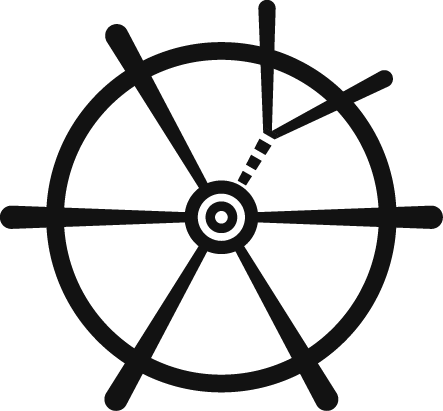
\includegraphics[height=17mm]{figs/SHiP-Symbol_Black} SHiP Collaboration}


\begin{abstract}
Status of the SHiP experiment and the Comprehensive Design Study (CDS) with focus on the re-optimization, the simulation studies, and the detector and physics performance. 
\end{abstract}

\keywords{SHiP, Comprehensive Design Study, CDS status report, CERN report.}

\maketitle

%%%%%%%%%%%%%%%%%%%%%%%%%%%%%%%%%%%%%%%%%%%%%%%%%%%%%%%%%%%%%%%%%
\begingroup\baselineskip.99\baselineskip
\tableofcontents
\endgroup
%%%%%%%%%%%%%%%%%%%%%%%%%%%%%%%%%%%%%%%%%%%%%%%%%%%%%%%%%%%%%%%%%

%\section{Introduction}
\label{sec:introduction}

A letter of intent \cite{Bonivento:2013jag} for a new experiment at CERN intended to search for hidden particles with the use of intensive beam of protons of SPS accelerator was submitted to SPSC  in 2013.  The SHiP collaboration that has been formed as a result prepared in 2015 two documents describing the physics case \cite{Alekhin:2015byh},  and a technical proposal \cite{Anelli:2015pba} of SHiP. The present paper provides an update of  the physics case and describes developments and advances in the technical design of the proposed experiment.

\section{Overview of changes since Technical Proposal}

\subsection{Physics Landscape}

{\bf Physics landscape in 2015.}  The discovery of the Higgs boson at the LHC in 2012 \cite{ATLAS:2012ae,Aad:2012tfa,Chatrchyan:2012tx,Chatrchyan:2012ufa}  made the Standard Model (SM) of elementary particles complete - all the particles predicted by it have been found, and their interactions,  tested at the LHC till now,  are consistent with those predicted by the SM. The triumph of the SM in particle physics is accompanied by the success  of the standard cosmological model based on Einstein's General Relativity -- $\Lambda$CDM, allowing to describe the structure of the Universe by a small number of parameters.

The quest for the new particles has not ended, however. Indeed we are certain that the SM is not complete. Several well-established observational phenomena -- neutrino masses and oscillations, dark matter, and baryon asymmetry of the Universe -- cannot be explained with known particles alone and clearly indicate that more particles should exist. Unfortunately, we do not have a definite prediction where to find this New Physics (NP), what masses, spins, and coupling constants these new particles should have. The era of guaranteed discoveries in particle physics has finished  with the detecting of the Higgs boson: for the particular value of the Higgs mass revealed by the LHC, the Standard Model remains mathematically consistent and valid as an effective field theory up to a very high energy scale, possibly all the way to the scale of quantum gravity, the Planck scale~\cite{Buttazzo:2013uya,Degrassi:2012ry,Bezrukov:2012sa,Bezrukov:2014ipa,Bezrukov:2014ina}.

{\bf Physics landscape in 2018.} \emph{In the last 3 years this picture did not change}.   The first ever run of proton-proton collisions at 13~TeV center-of-mass energies (LHC Run 2 will finish in October 2018) has uncovered no significant deviations from the Standard Model~\cite{ICHEP2018_ATLAS,ICHEP2018_CMS,CMSSUSY,ATLASSUSY,ATLASexotics,CMSexotics,ICHEP2018_exotics,ICHEP2018_SUSY}. Nor did so other direct searches for new physics at particle physics laboratories worldwide. The intriguing hints of lepton flavour universality violations in semi-leptonic B decays have been reported in the recent years by Belle and LHCb~\cite{Huschle:2015rga,Sato:2016svk,Hirose:2016wfn,Aaij:2015yra,Aaij:2017uff}. Even if these hints are confirmed, it will not be possible to determine the scale of NP with certainty. Possible explanations can involve particles of very different masses, including heavy particles (that can be beyond the reach of the LHC or HL-LHC) as well as the light ones with masses $\mathcal{O}(100)$~MeV or even $\mathcal{O}(\mathrm{keV})$, see e.g.~\cite{He:2017bft,He:2012zp,Robinson:2018gza,Azatov:2018kzb}.

Significant advances in neutrino physics of the recent years~\cite{ICHEP2018_neutrino,ICHEP2018_neutrino_theory} did not improve our knowledge about the scale of new particles that drive neutrino masses and oscillations. In particular the simplest model with only two sterile neutrinos of essentially any mass can accommodate the data of all neutrino experiments, including future measurements of the CP-violating parameter.

With regard to Dark Matter, the absence of detections in direct or indirect search experiments for weakly interacting massive particles (WIMPs) in GeV-TeV mass range stimulated growing attention to light dark matter candidates: sterile neutrinos, axions, WIMP-like particles but with lower (sub-GeV) masses etc and corresponding experimental efforts to search for such particles~\cite{ICHEP2018_DM,Duffy:2009ig,Boyarsky:2018tvu}. At the same time, in cosmology significant attention was attracted to light non-WIMP dark matter models including detailed studies of cosmological structure formation for these models as well as systematic searches for various signatures of such particles in cosmological and astrophysical observations; detailed description of baryogenesis and the physics of early Universe with such particles etc. The ``cosmologically interesting'' areas of the parameter spaces were significantly improved.

\bigskip

\emph{To summarize}, the current results in theoretical and experimental particle physics, cosmology and  astrophysics leave still the parameters of NP largely undetermined.

The fact that no convincing signs of new particles have been found so far suggests that that they are either heavier than the reach of the present days accelerators or interact very weakly.

The current experimental situation thus defines three main and fully complementary directions of development of particle physics:
\begin{enumerate}
    \item  The  direct searches of NP, namely the search for new phenomena occurring at high (untested) energies, such as the production of new types of particles (\emph{energy frontier}).
    \item  The indirect searches of NP, namely the search for possible failures in the SM predictions when performing high-precision experiments at any energy scale (\emph{precision frontier}).
\item The searches of extremely feebly interacting relatively light particles (\emph{intensity frontier}).
\end{enumerate}

\begin{figure}[!t]
    \centering
    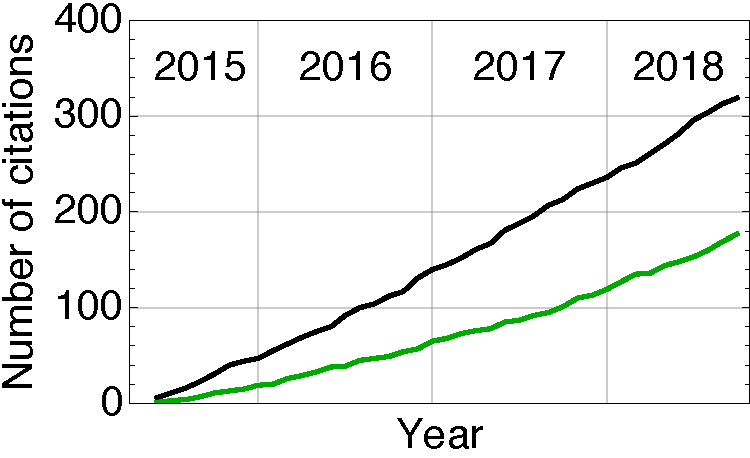
\includegraphics{figs/Introduction/citations_PP_TP.pdf}
    \caption{Citation history of the SHiP physics paper~\protect\cite{Alekhin:2015byh} (black) and of the SHiP Technical Proposal \protect\cite{Anelli:2015pba} since their initial publication in April 2015.}
    \label{fig:citations}
\end{figure}

While energy frontier is investigated at the LHC and drives the projects of the future colliders, the precision frontier is pursued at LHCb and elsewhere, the intensity frontier remains under-explored. It is the main goal of the SHiP experiment to make the break-through in this direction. In particular, the discovery potential of SHiP will allow to  explore the domain of  particle masses and couplings that are not accessible to the energy and precision frontier experiments and potentially find the particles that lead to neutrino masses and oscillations, explain  baryon asymmetry of the Universe and  shed the new light on the properties of dark matter (for a detailed discussion see \cite{Alekhin:2015byh}), even more so with the updated SHiP design described below.

SHiP experiment has received lots of attention from the particle physics community. The SHiP physics paper~\cite{Alekhin:2015byh} is a highly-cited document (see Fig.~\ref{fig:citations}),  many groups continue to explore the scientific potential of the experiment, making detailed predictions for models of feebly interacting particles.
Apart from the SHiP experiment, several dedicated intensity frontier experiments have been proposed in the recent years: CODEX-b~\cite{Gligorov:2017nwh},
MATHUSLA~\cite{Chou:2016lxi,Curtin:2017izq,Evans:2017lvd},
FASER~\cite{Feng:2017uoz,Feng:2017vli,Kling:2018wct}. Recognizing the importance of non-LHC physics, the CERN Management created in 2016 a dedicated Study Group “Physics Beyond Colliders” (PBC). 
Searches of heavy neutral leptons, dark photons, dark scalars and other super-weakly interacting light particles has been included in the scientific goals of many presently running experiments~\cite{Aaij:2014aba,Khachatryan:2015gha,Aad:2015xaa,Sirunyan:2018mtv,Izmaylov:2017lkv, Mermod:2017ceo,CortinaGil:2017mqf,Antusch:2017hhu,Drewes:2018gkc,Liventsev:2013zz,Kwon:2017anc,TheBelle:2015mwa,Lees:2017lec,Banerjee:2016tad,Aaboud:2018jbr,Aaij:2017rft}.



\subsection{Global concept of re-optimized experimental configuration}

\subsubsection{Muon shield}
Magnetized hadron stopper

\subsubsection{{Decay volume}}
Pyramidal frustum

\subsubsection{Detector layout}
Main changes to scattering spectrometer and decay spectrometer

\section{Beam line}
\label{sec:beamline}

\begin{itemize}
    \item beam extraction
    \item proton sharing
    \item operation in bunched mode (if	there are hints for LDM
    signal from emulsion spectrometer)	
    \item spill structure
    \item beam line with TauFV
    \item target complex
    \item target, extended to 12 lambda, prototype in beam
    \item magnetization of hadron stopper
    \item facility/experiment interface
    \item free standing muon shield, optimization using machine learning, field map, technology studies and tests
    \item Vacuum vessel layout engineering (decay volume + spectrometer section)
    \item experimental area updated layout + infrastructure
    \item updated detector layout
    \item experiment services and integration
    \item detector installation scheme
\end{itemize}

\begin{figure}[th]
\centering
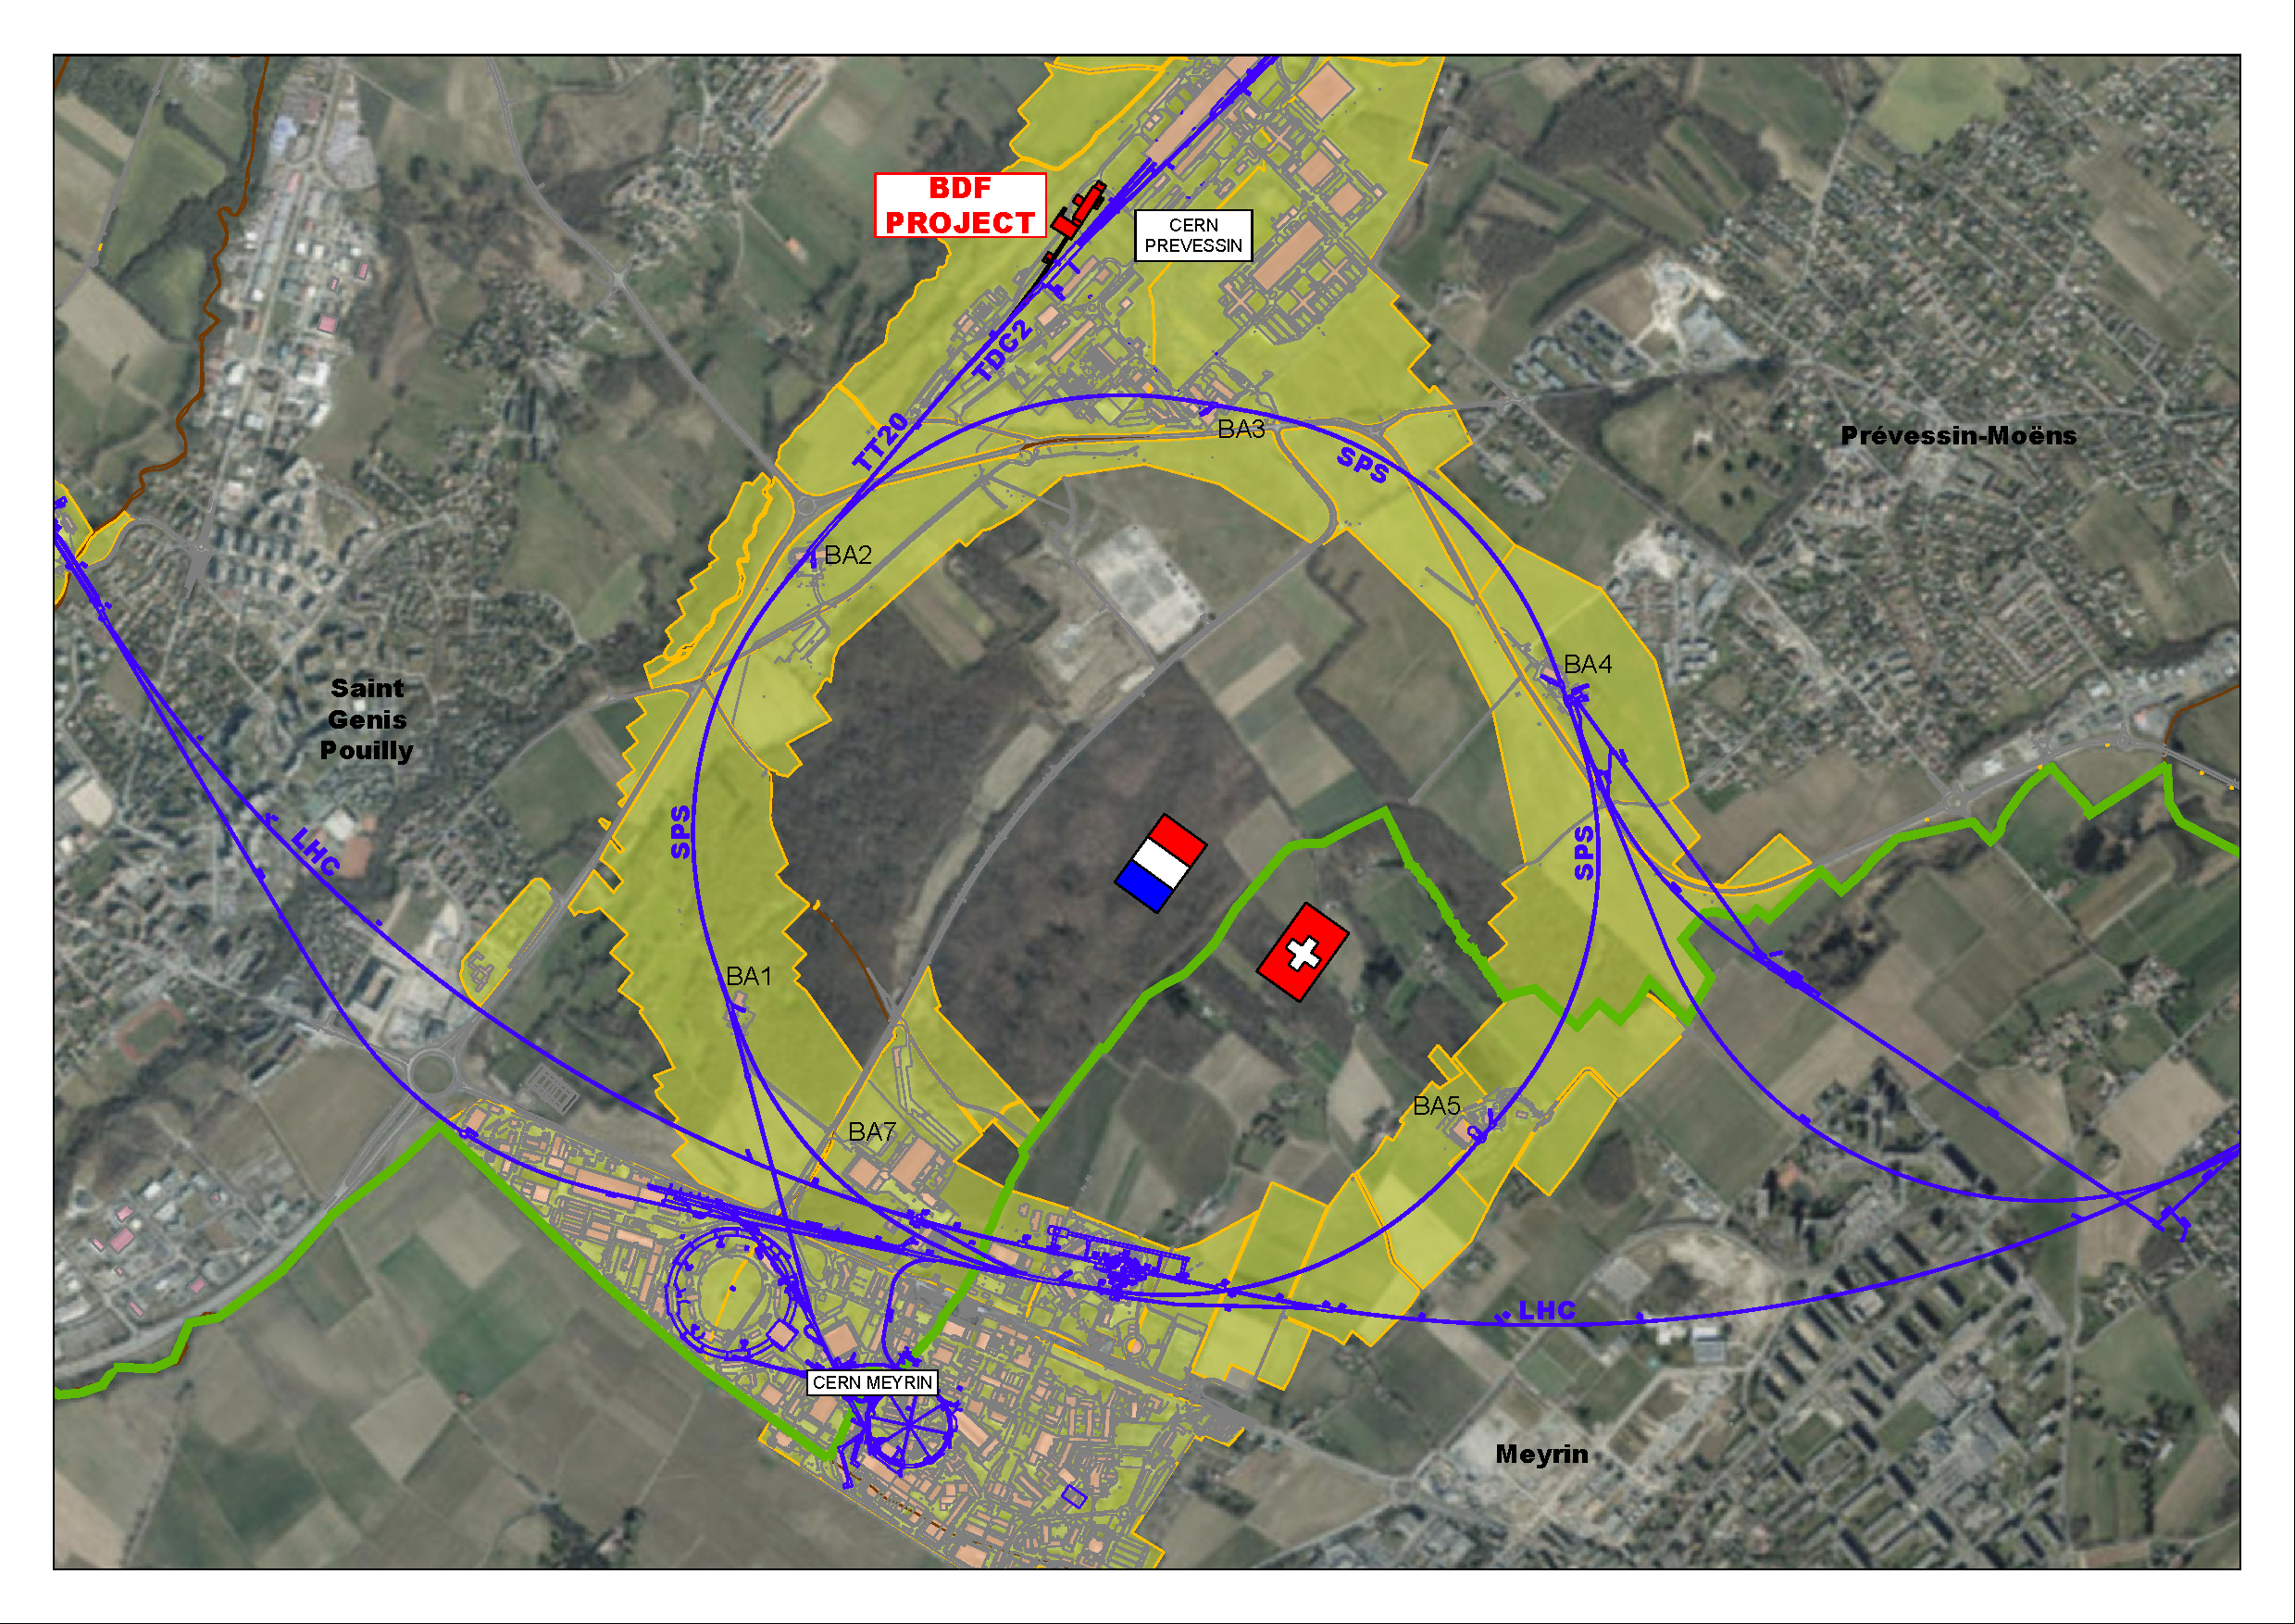
\includegraphics[width=1.0\columnwidth]{figs/BeamLine/20180529-BDF-General_figure_for_BDF_paper.pdf}
\caption{}
\label{fig:FacilityLocation}
\end{figure}

\begin{figure}[th]
\centering
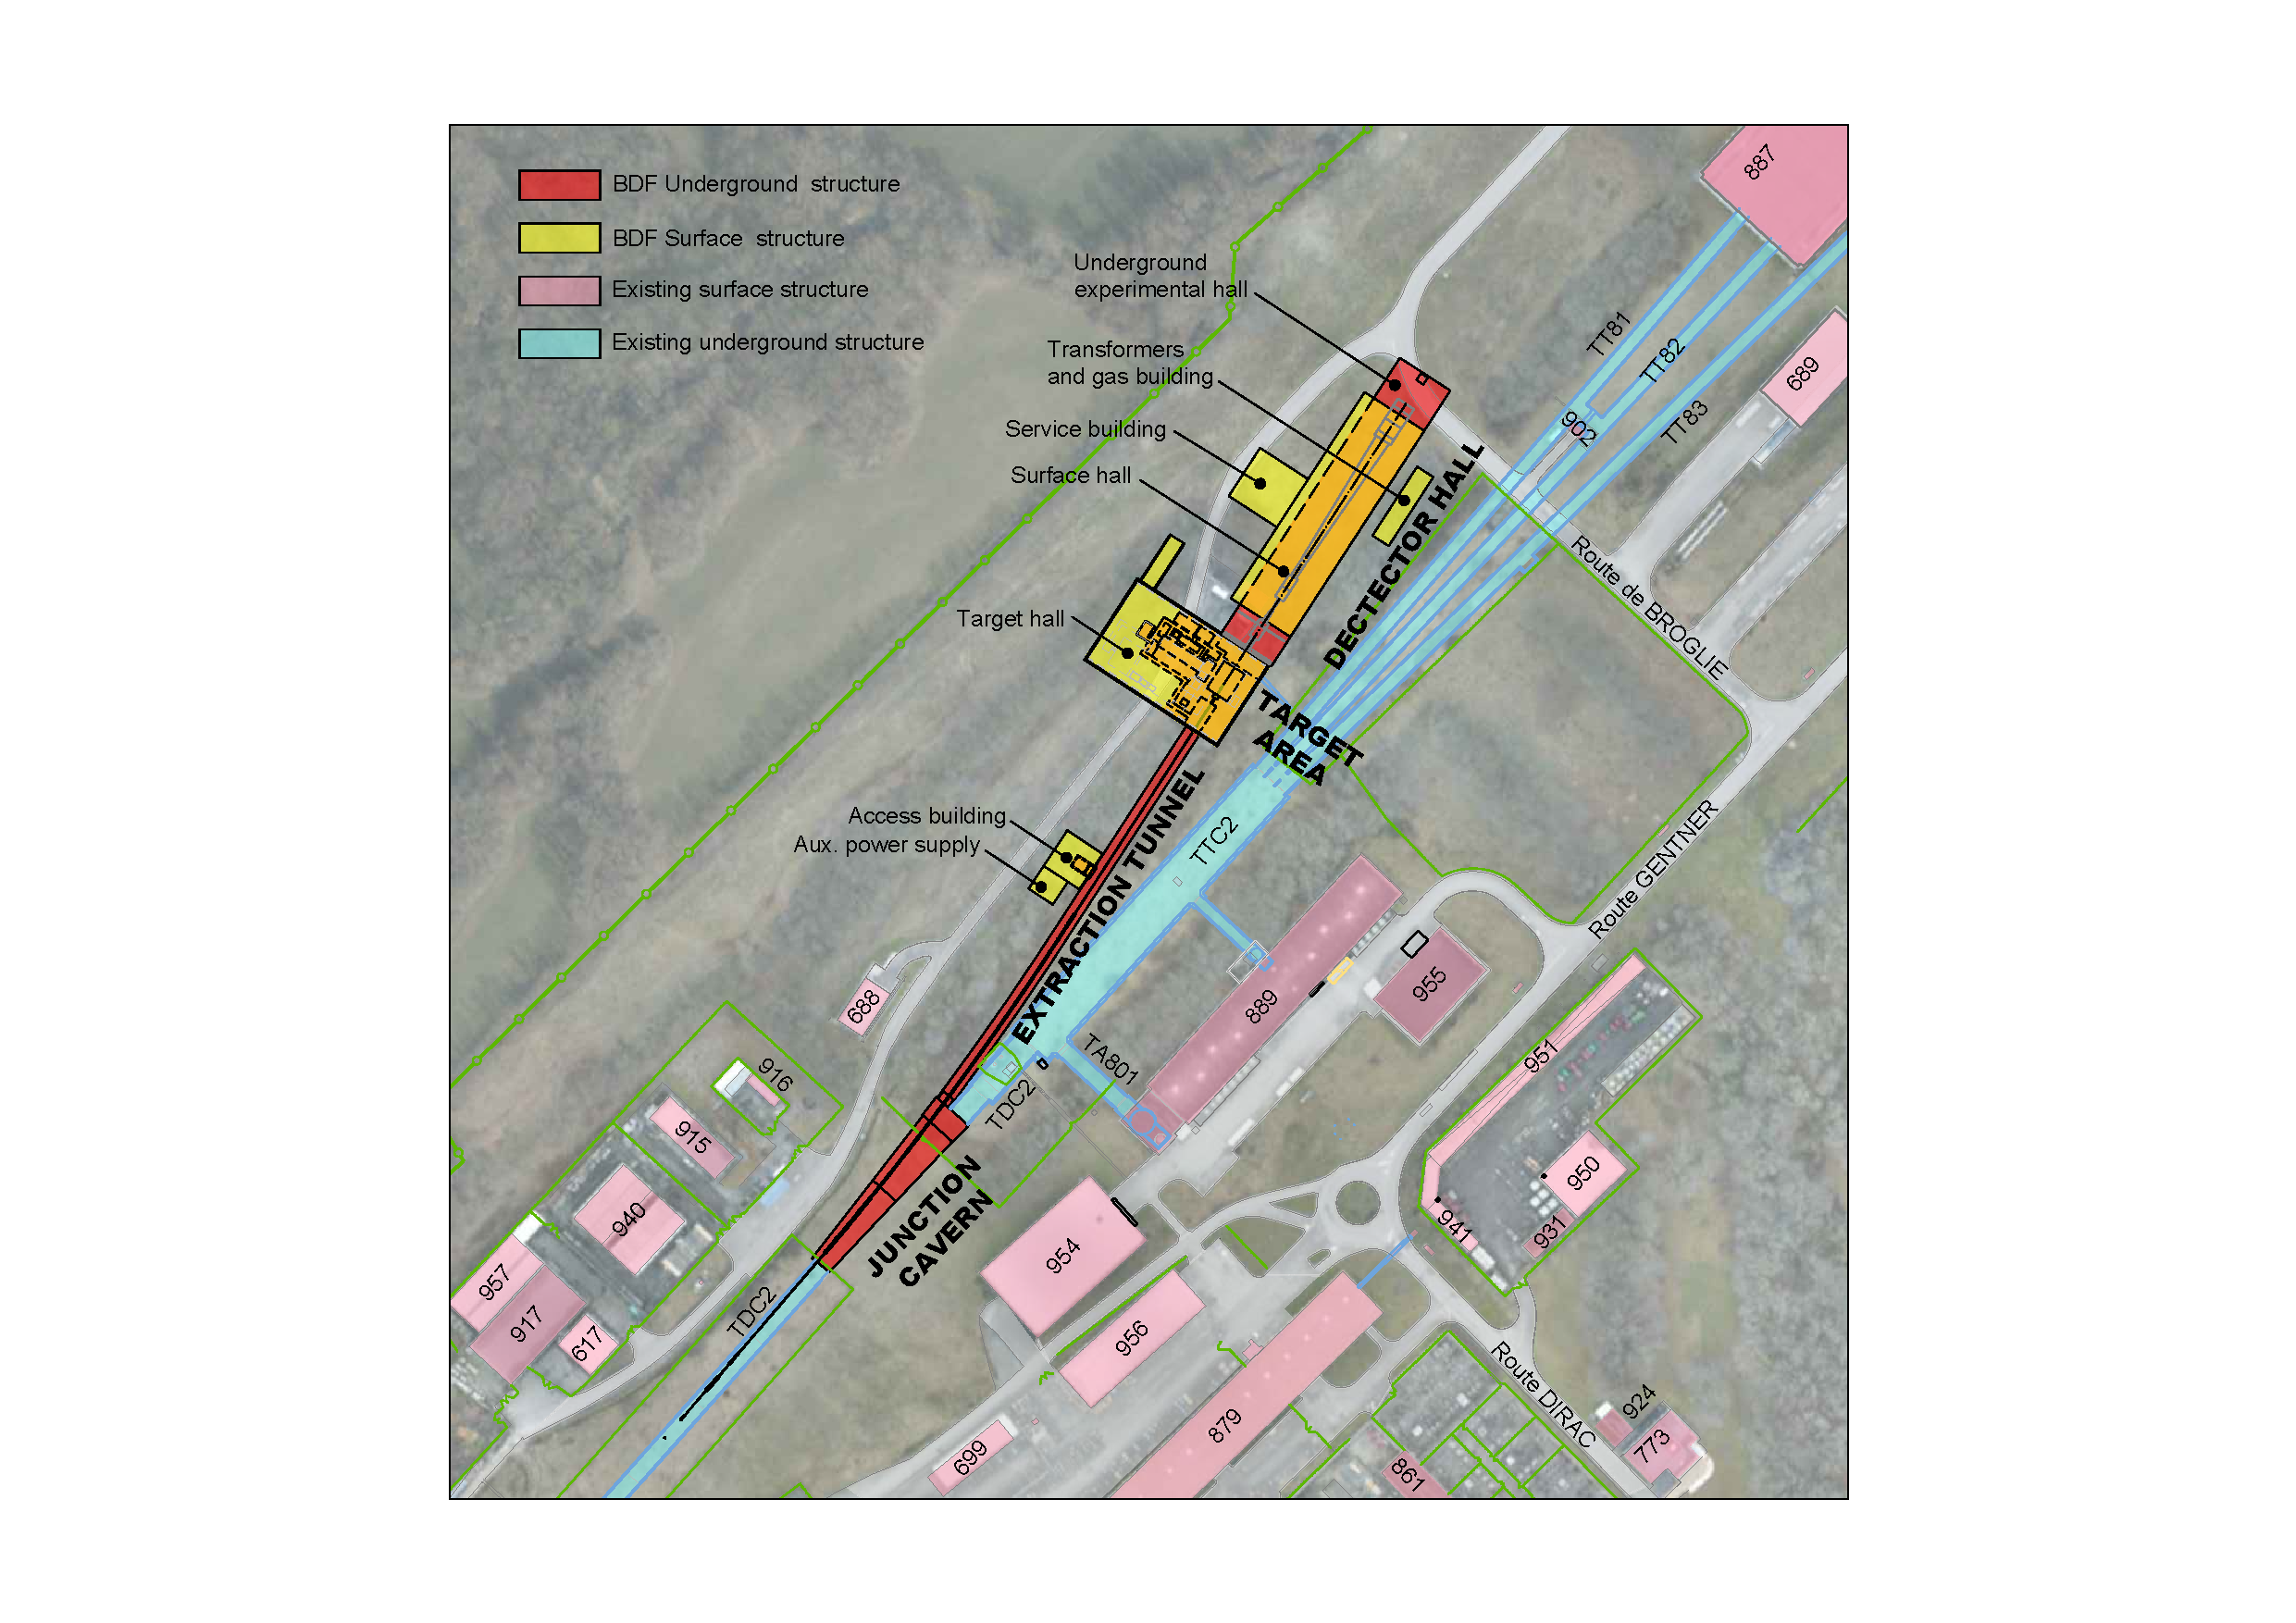
\includegraphics[width=1.0\columnwidth]{figs/BeamLine/20180529-BDF-Figure_for_BDF_paper.pdf}
\caption{}
\label{fig:FacilityLocation}
\end{figure}

\begin{figure}[th]
\centering
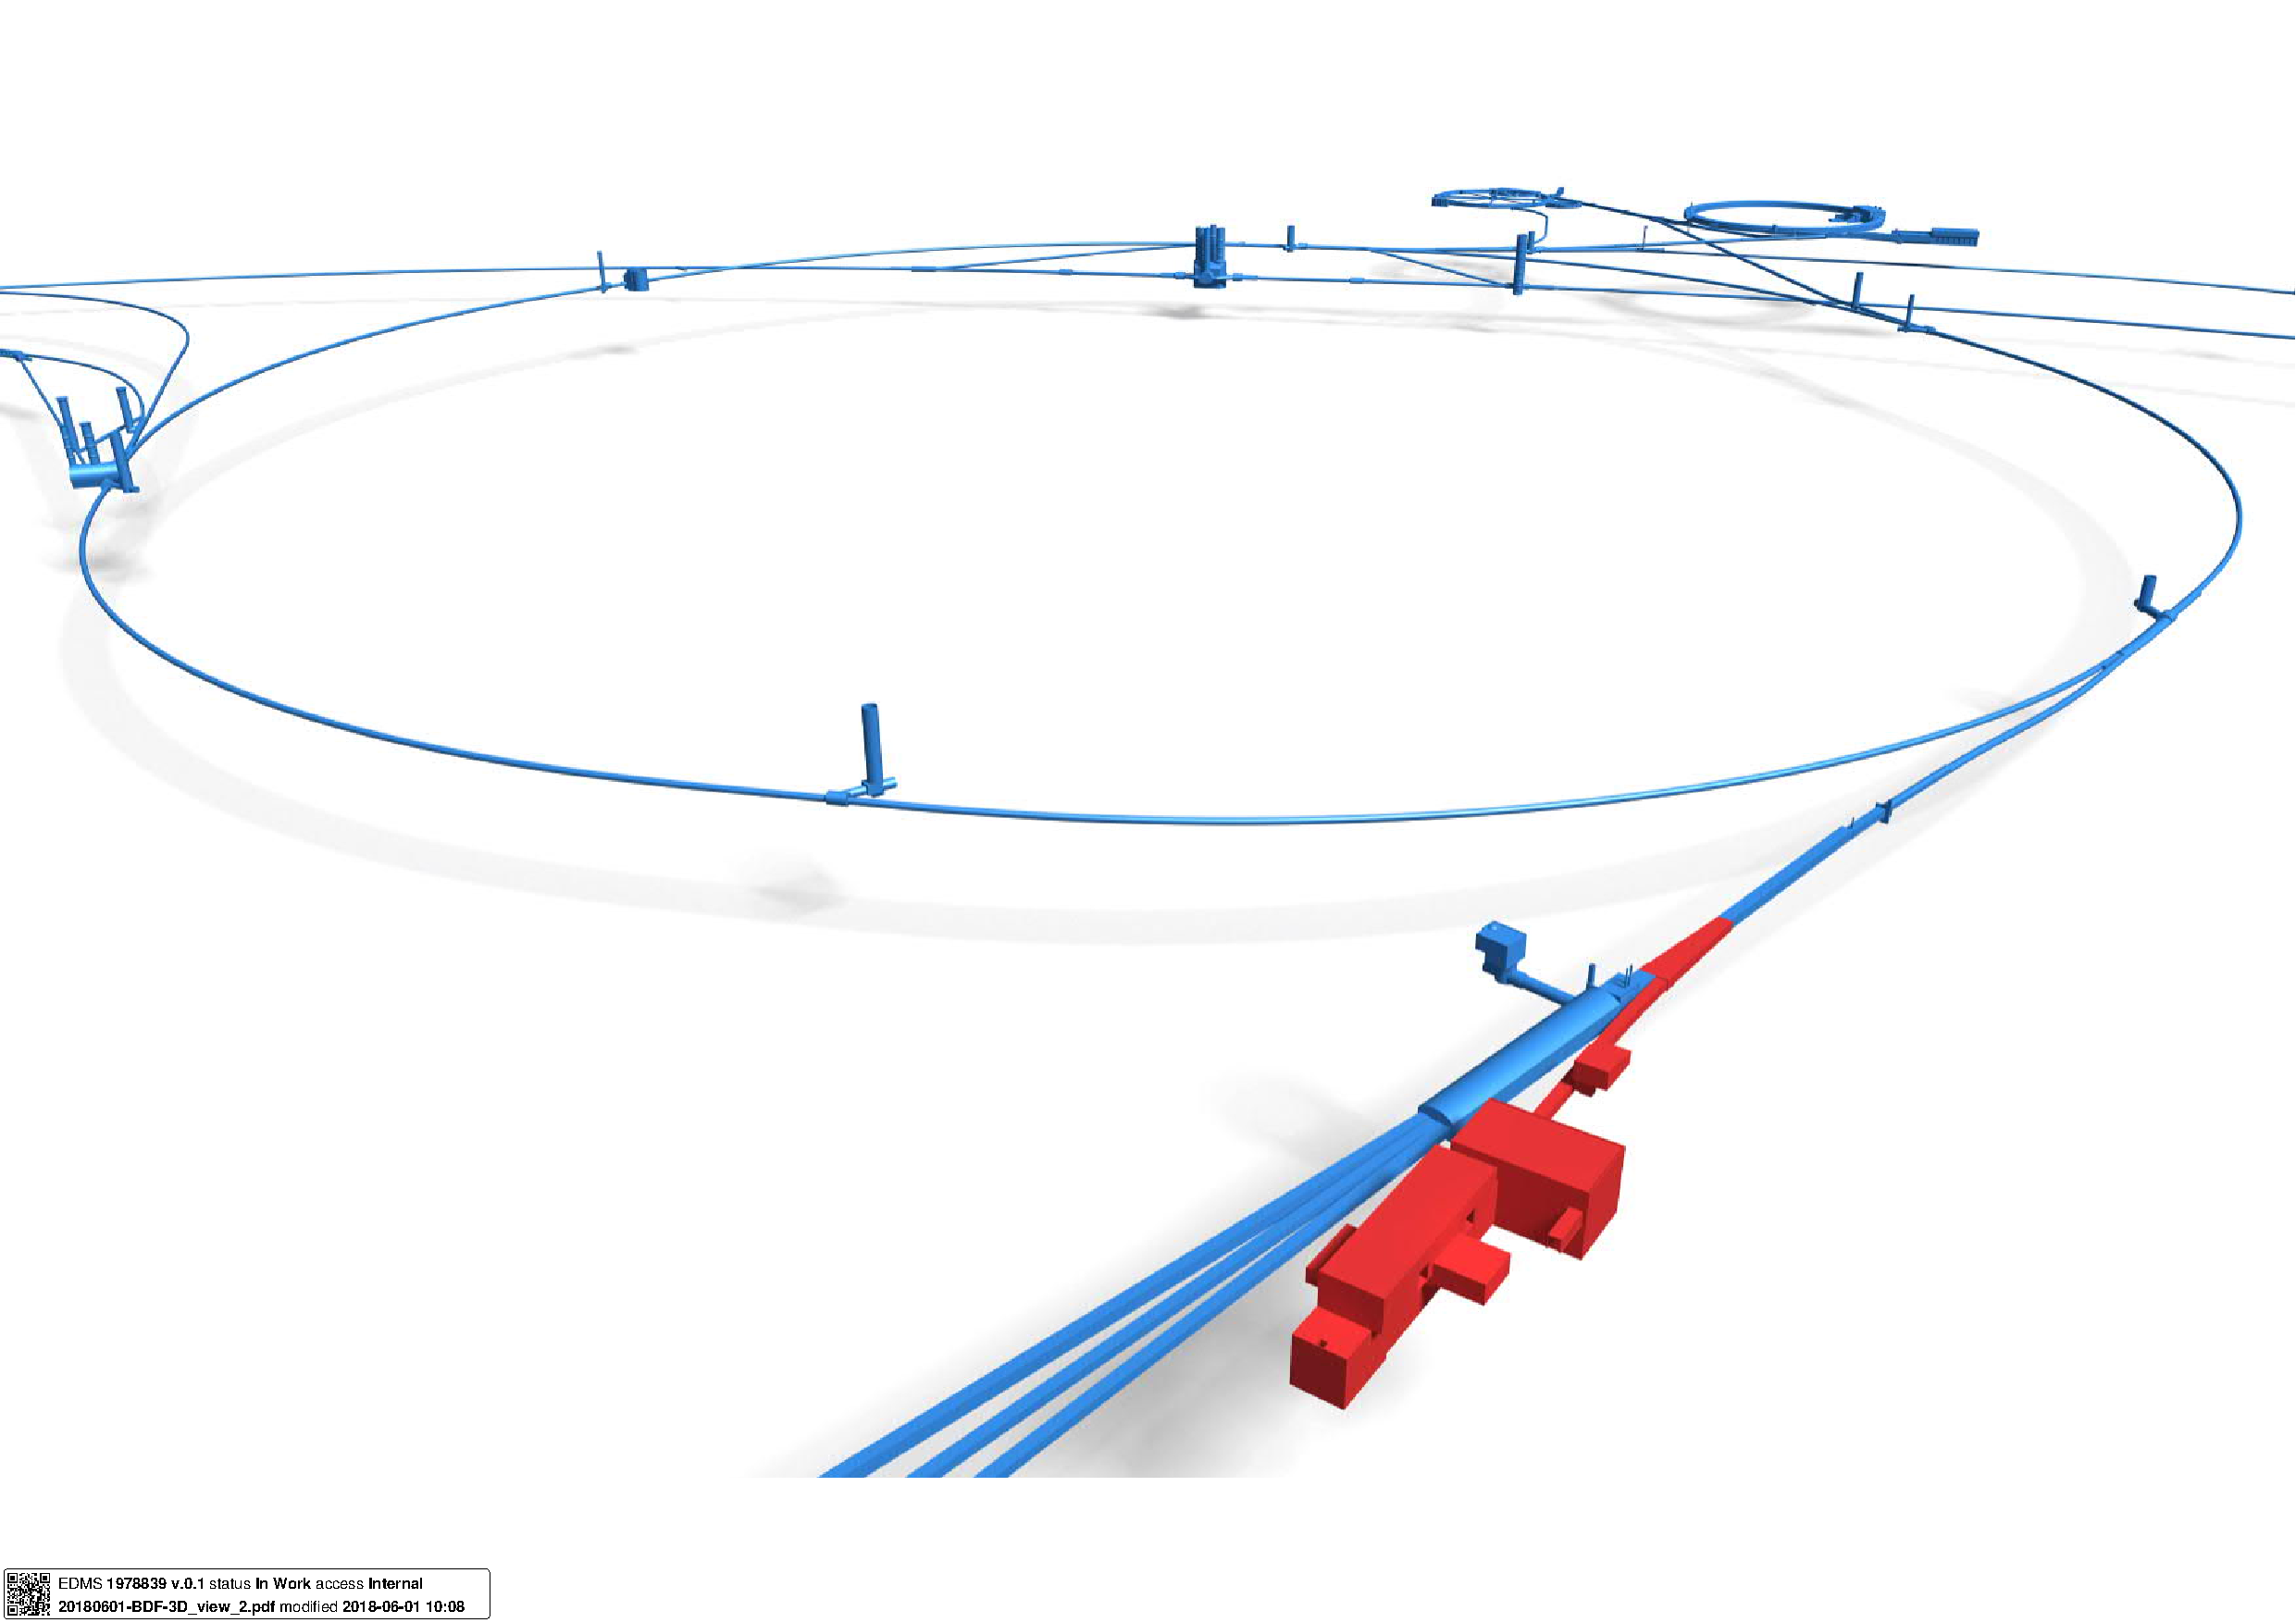
\includegraphics[width=1.0\columnwidth]{figs/BeamLine/20180601-BDF-3D_view_2.pdf}
\caption{}
\label{fig:FacilityAccComplex}
\end{figure}

The Comprehensive Design Study for the experimental facility has been carried out by the 
Beam Dump Facility working group and in its dedicated subgroups in the context of the Physics Beyond Collider Study Group in 
close collaboration with the SHiP experiment.  

Based on the request put forward in the addendum to the SHiP Technical Proposal~\cite{ref:ship_tp_add}, this study phase has 
consisted in a detailed elaboration of the SHIP operational scenario, and in a preliminary design of the main components of the 
proton delivery, the target and the target complex, and the experimental area, together with a detailed evaluation of the 
radiological aspects and mitigation. Several critical items have been prototyped to demonstrate the concepts, the new type of 
three-way combined beam splitter/kicker magnet and the target and a conceptual version of its enclosure.

In addition, it has been considered of high importance to perform a preliminary study of
the integration of the whole complex, civil engineering design and execution process in order to produce a more precise cost 
estimate and time line for the project.

A full writeup of the Comprehensive Design Study for the Beam Dump Facility is available~(\cite{ref:bdf_yellowreport} and references therein).

Assumptions and baseline parameters confirmed.

The sections below summarizes the changes, updated requirements, status and key conclusions related to the experimental facility and beam line.

Reference to feasibility studies in TP addendum and BDF working group, focus on re-optimization and updates, synthesis of conclusions BDF work



\section{Proton yield and beam delivery}

The SHiP operational scenario is based on a similar fraction of beam time as the past CERN Neutrinos to Gran Sasso (CNGS) program. The most favourable experimental conditions for SHiP are obtained with a proton beam energy of around 400 GeV. A nominal beam intensity of $4\times10^{13}$ protons on target per spill is assumed for the design of the experimental facility and the detector. In the baseline scenario, the beam sharing delivers an annual yield of $4\times 10^{19}$ protons to the SHiP experimental facility and a total of $10^{19}$ to the other physics programs at the CERN North Area, while respecting the beam delivery required by the LHC and HL-LHC . The physics sensitivities are based on acquiring a total of $2\times 10^{20}$ protons on target, which may thus be achieved in five years of nominal operation.

Significant progress has been made in the studies of techniques to reduce the beam losses 
and activation during the slow extraction process which is necessary to achieve the baseline 
intensity of $4\times 10^{19}$ protons on target per year. The current status confirms the 
intensity reach to within a factor of two, and further techniques presently under deployment 
are  aiming to provide the additional reduction to allow the full intensity.

\subsection{Operation with slow-extraction in bunched mode}

SHiP profits from the unique feature in the SPS of slow extraction of a de-bunched beam over a timescale of around a second. It allows tight control of combinatorial background, and allows diluting the large beam power deposited on the proton target both spatially and temporally. Should an observation require consolidation, a second mode of operation with slow extraction of bunched beam is also foreseen in order to further increase the discrimination between the signature of a Light Dark Matter object, by measuring their different times of flight,  
%in the mass range $0.5{-}6~\gevcc$ 
and background induced by neutrino interactions.

\section{Target system}

Target extended from 10 to 12 interaction lengths, radius changed from square block 30x30 to cylindrical with radius of 12.5cm.

% SHiP uses a target of 12 interaction lengths of molybdenum-tungsten 
% which has been designed to cope with % the large beam power and which 
% maximize the production % of charm and beauty hadrons, and the 
% production and % interactions of photons, while minimizing the production 
% of neutrinos from pion and kaon decays. The infrastructure complex to 
% house the proton target with the associated services and remote handling, 
% and which is fully compatible with the radiation protection and 
% environmental considerations, has been taken through an advanced feasibility 
% study.

\section{Updated experiment layout}

The main experimental challenge concerns the requirement of highly efficient reduction of beam-induced backgrounds to below $0.1$ events in the projected sample of $2\times 10^{20}$ protons on target. To this end, the experimental configuration includes a unique design of a muon shield based on magnetic deflection to reduce the flux of muons emerging from the target by six orders of magnitude in the detector acceptance. 

The SHiP experiment incorporates two complementary apparatuses. The first detector
immediately downstream of the muon shield consists of an emulsion based spectrometer optimised for recoil signatures of hidden sector particles and $\tau$ neutrino physics.


\subsection{Magnetization of the target hadron stopper}
Contract and activity with RAL

\subsection{Free-standing Muon shield}

The design and performance of the muon shield poses certain technological challenges. These 
include how to best assemble sheets of Grain Oriented steel without disrupting the magnetic 
circuit, how to cut the GO sheets into desired configurations, and how to best connect the 
GO sheets to achieve the desired stacking factor. In order to address these questions a 
prototyping campaign is underway.

The design of the muon shield and the residual rate of muons depends on the momentum 
distribution of the muons produced in the initial proton collision. The latest shield 
optimisation and rate estimates were performed using \texttt{PYTHIA} simulations. In order 
to validate these simulations a test beam campaign is starting in July to measure the muon 
flux using a replica of SHiP's target. Further details can be found in Ref.~[SHiP-EOI-016]. 
Depending on the outcome of this test beam campaign, a further optimisation of the 
shield configuration will be performed.

\begin{figure}[thbp]
\centering
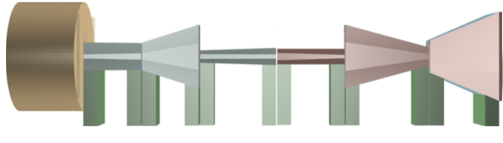
\includegraphics[width=1.0\columnwidth]{figs/BeamLine/shield_YZview.png}
\caption{Side view of the optimized muon shield magnets.}
\label{fig:shieldSideView}
\end{figure}

\begin{figure}[thbp]
\centering
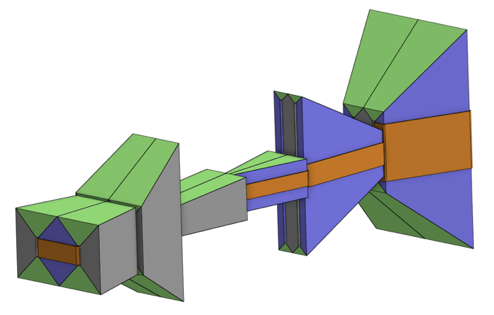
\includegraphics[width=0.8\columnwidth]{figs/BeamLine/shield_3dview.png}
\caption{3D view of the optimized muon magnetic shield.}
\label{fig:shieldSideView}
\end{figure}

\begin{figure}[thbp]
\centering
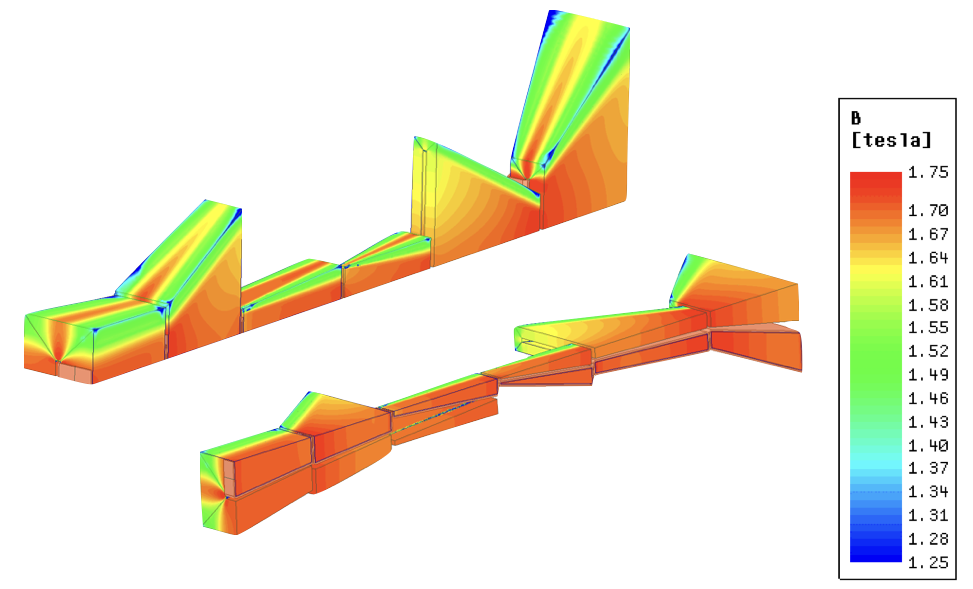
\includegraphics[width=0.8\columnwidth]{figs/BeamLine/shield_field_quadrant.png}
\caption{Modelled magnetic field distribution with nominal field intensity set to 1.7T. Quadrant cut out is shown.}
\label{fig:shieldMagneticField}
\end{figure}

\begin{figure}[thbp]
\centering
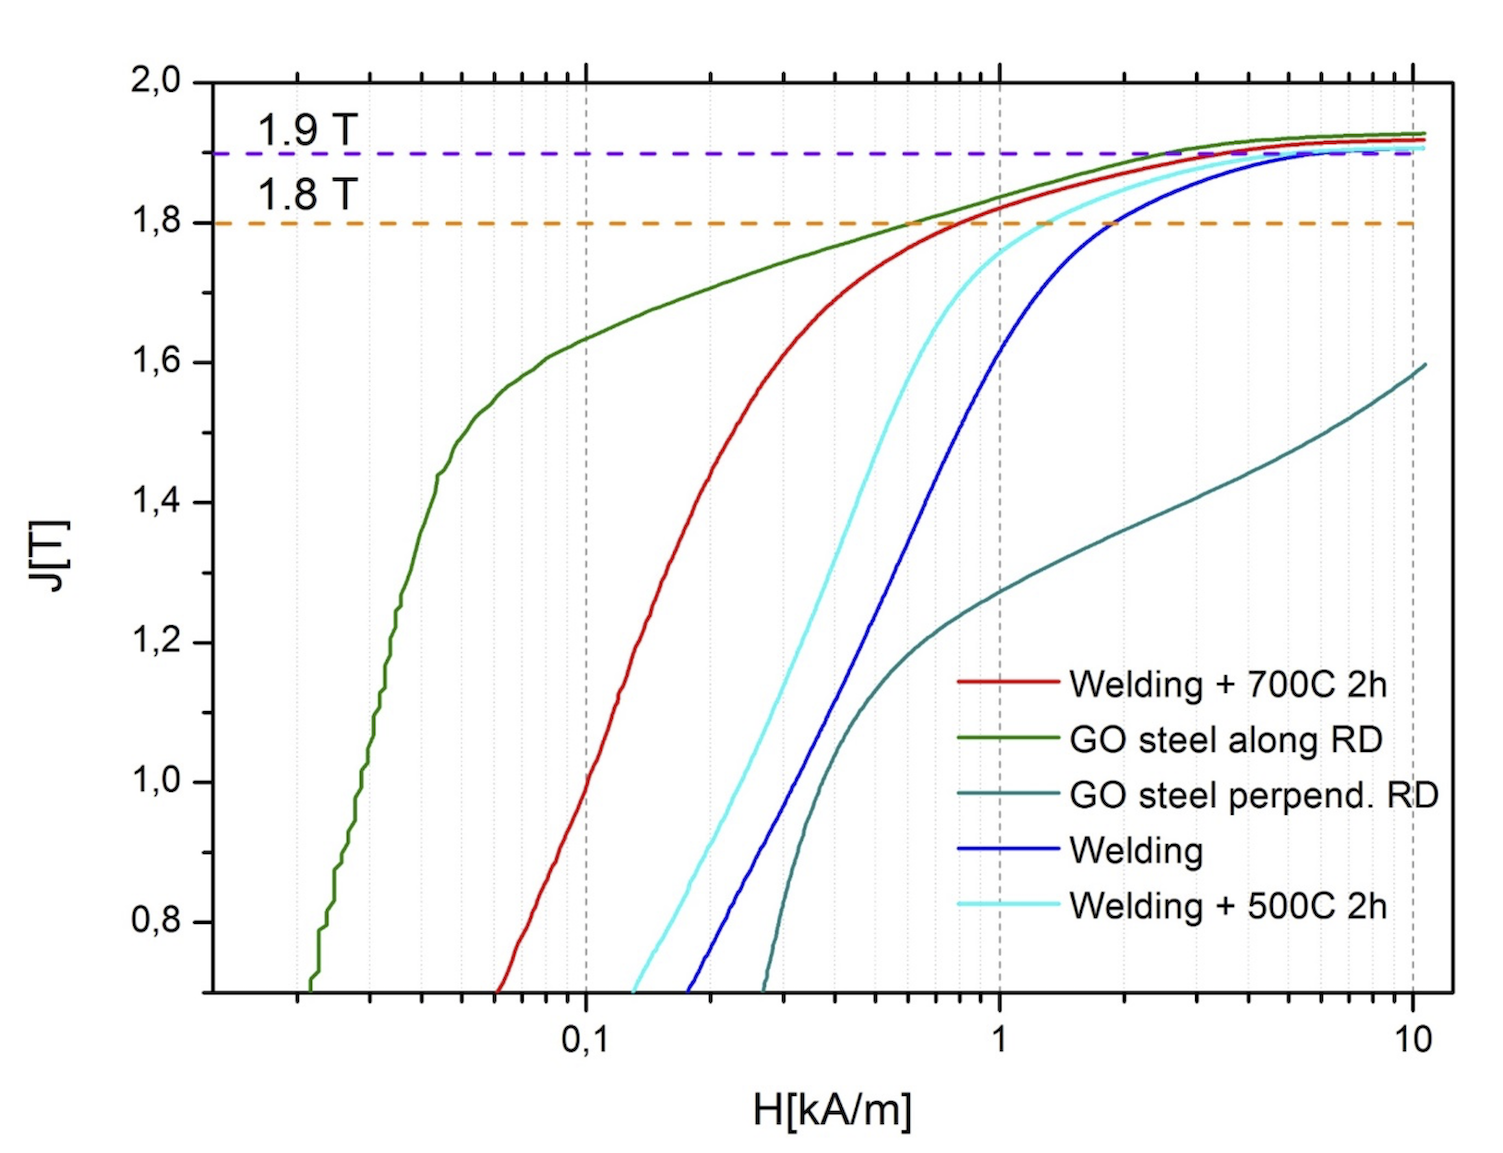
\includegraphics[width=0.8\columnwidth]{figs/BeamLine/go_steel_annealing.png}
\caption{Measured magnetic properties of the Grain Oriented steel batch: unprocessed sample along (green) and perpendicular (dark green) to rolling direction,
after the welding (blue), after the following annealing at $500^\circ$C (cyan) and $700^\circ$C (red).}
\label{fig:goSteelAnnealing}
\end{figure}

\begin{figure}[thbp]
\centering
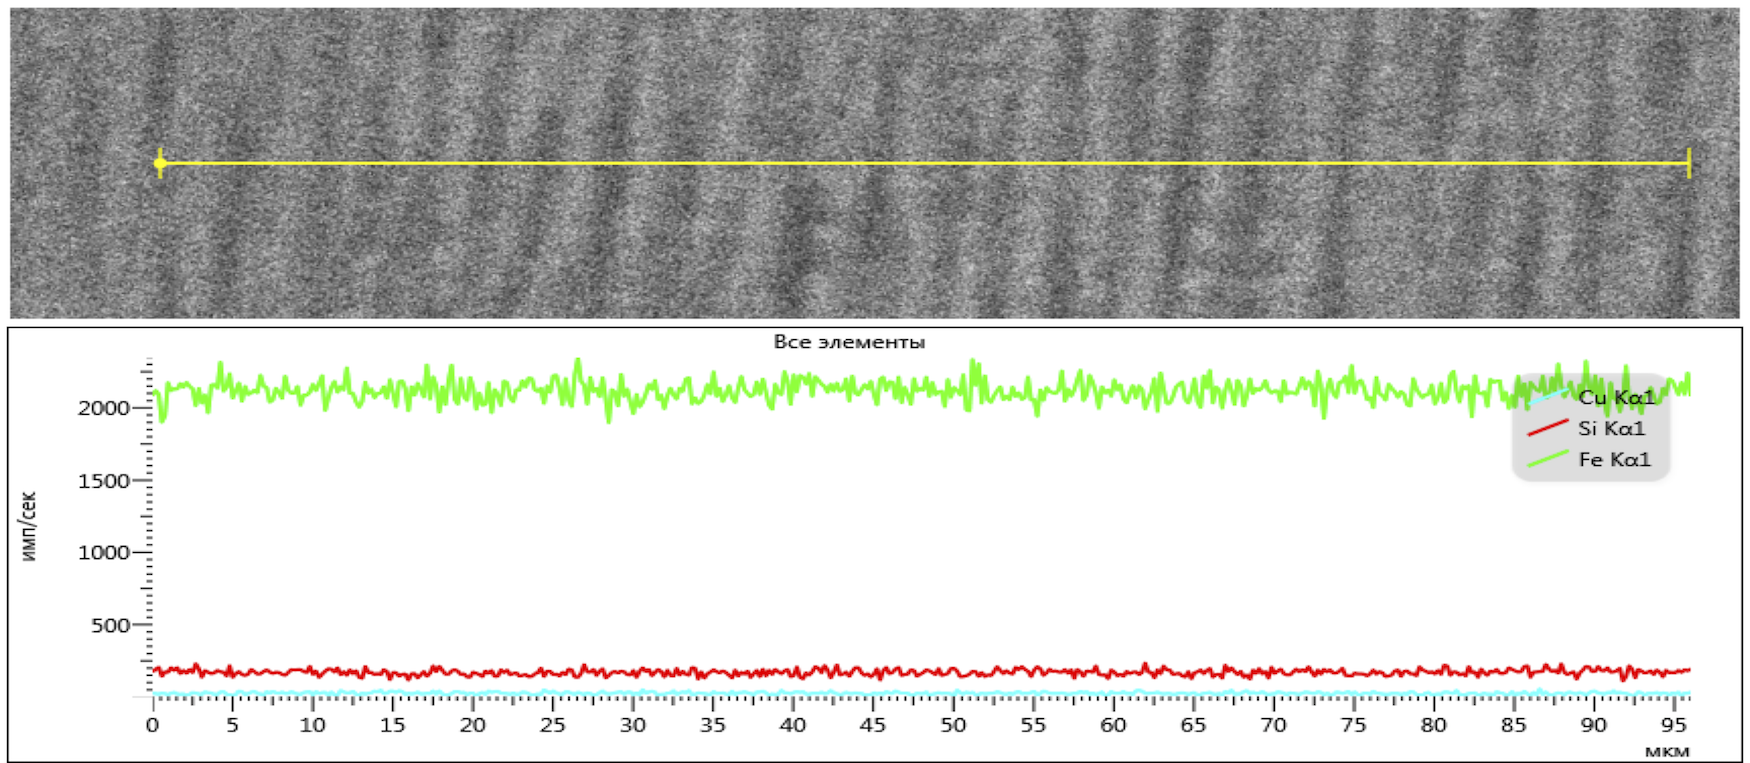
\includegraphics[width=0.45\columnwidth]{figs/BeamLine/carbon_structure.png}
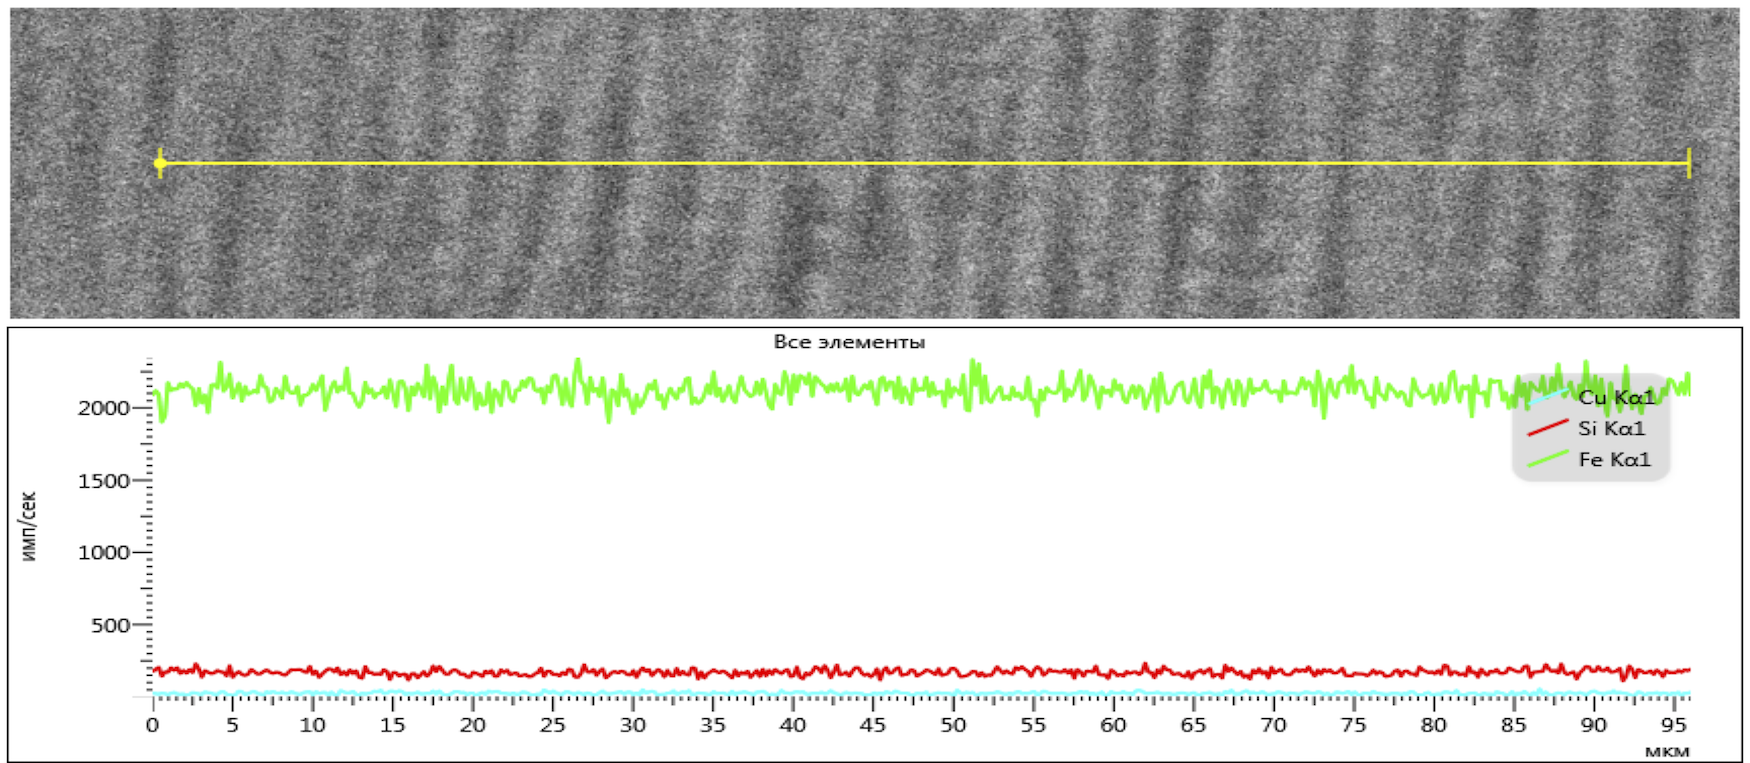
\includegraphics[width=0.45\columnwidth]{figs/BeamLine/carbon_structure.png}
\caption{Carbon structure in the welded joint before (left) and after (right) \em{(to be updated)} annealing.}
\label{fig:goCarbonStructure}
\end{figure}

\begin{figure}[thbp]
\centering
%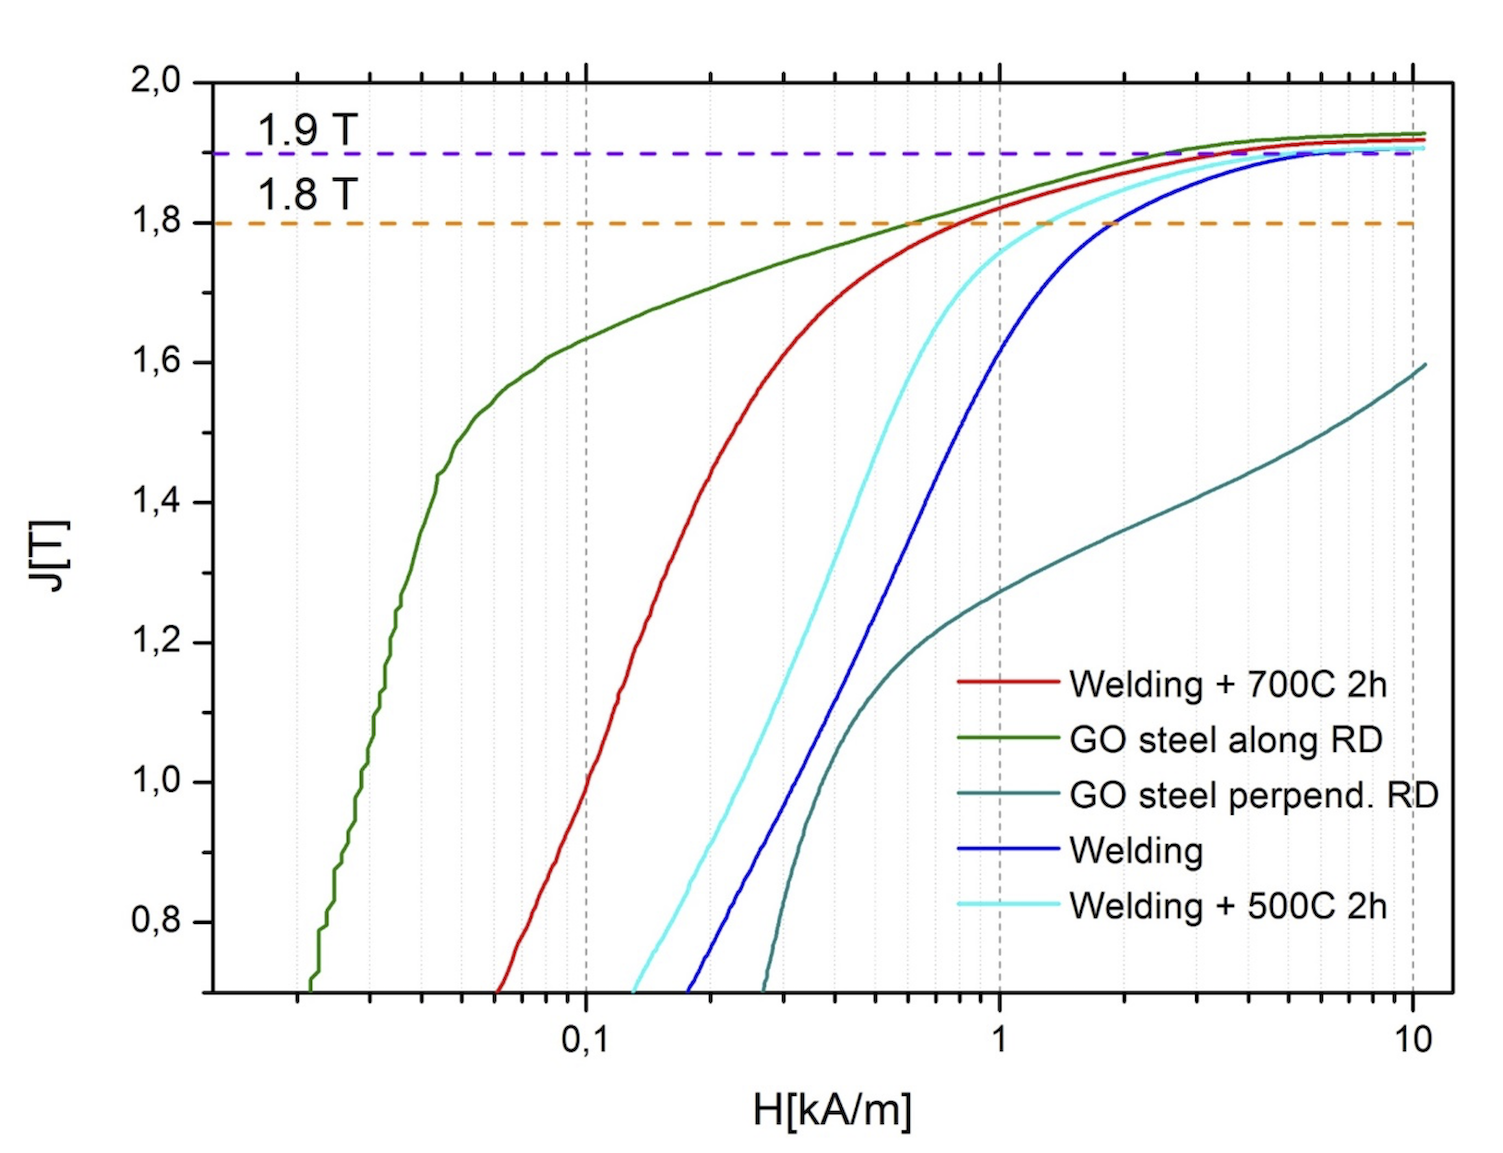
\includegraphics[width=1.0\columnwidth]{figs/BeamLine/go_steel_annealing.png}
\caption{Simulated hit rates caused by muons passing magnetic shield. Comparison of  ideal magnetic field setup (red) and realistic magnetic field (blue).}
\label{fig:shieldHitsMap}
\end{figure}

\begin{figure}[thbp] 
\centering
%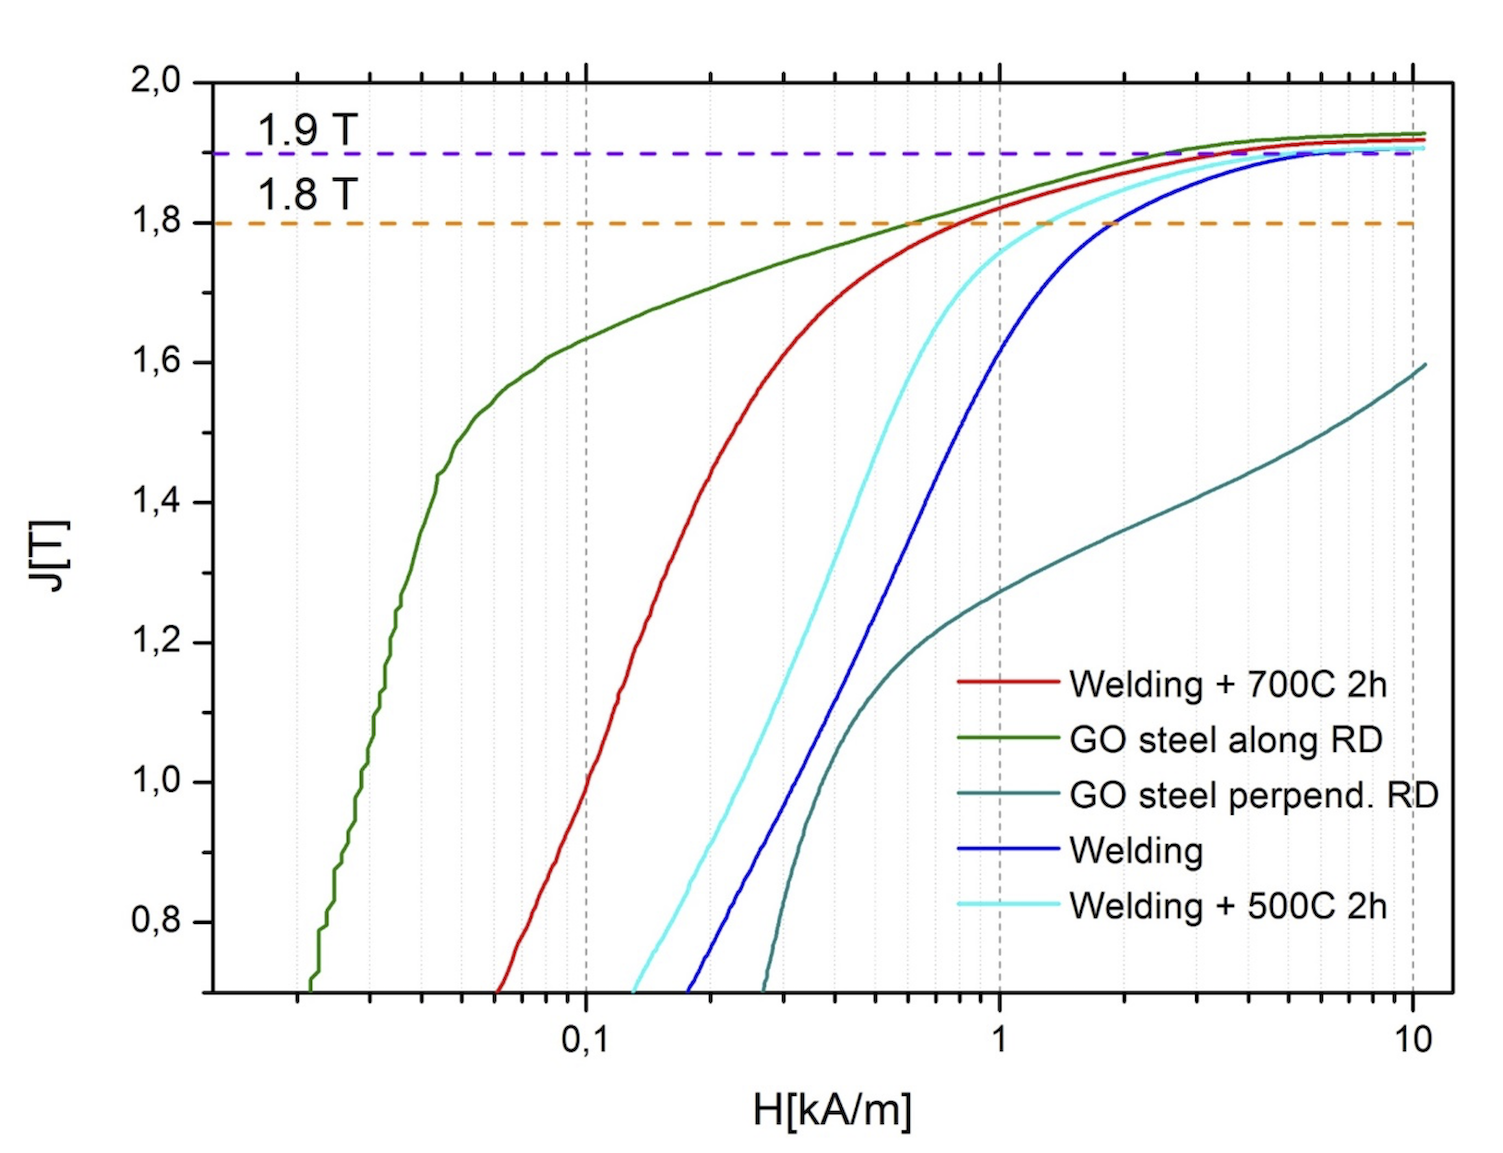
\includegraphics[width=1.0\columnwidth]{figs/BeamLine/go_steel_annealing.png}
\caption{Reconstructed track rates caused by muons passing magnetic shield. Comparison of  ideal magnetic field setup (red) and realistic magnetic field (blue).}
\label{fig:shieldTracks}
\end{figure}



\subsection{Vacuum vessel}
Baseline is a ....
Consist of several sections


The preliminary studies of the vacuum system for the approximately 1750 $m^3$ SHiP vacuum vessel 
shows that the requirements can be satisfied with a system of combined root-screw pumps, piezo 
and membranes gauges for pressure monitoring and manual valves for operation and venting 
purposes~\cite{ref:vacuumsystem}(EDMS 2000025). 
A low outgassing epoxy paint is considered to be deposited on the steel surface under vacuum in 
order to reduce the surface outgassing. The longitudinal vacuum forces which are taken into 
account in the design of the vacuum chamber are around 300t. 



\section{Experimental Area and Infrastructure}

\begin{figure}[th]
\centering
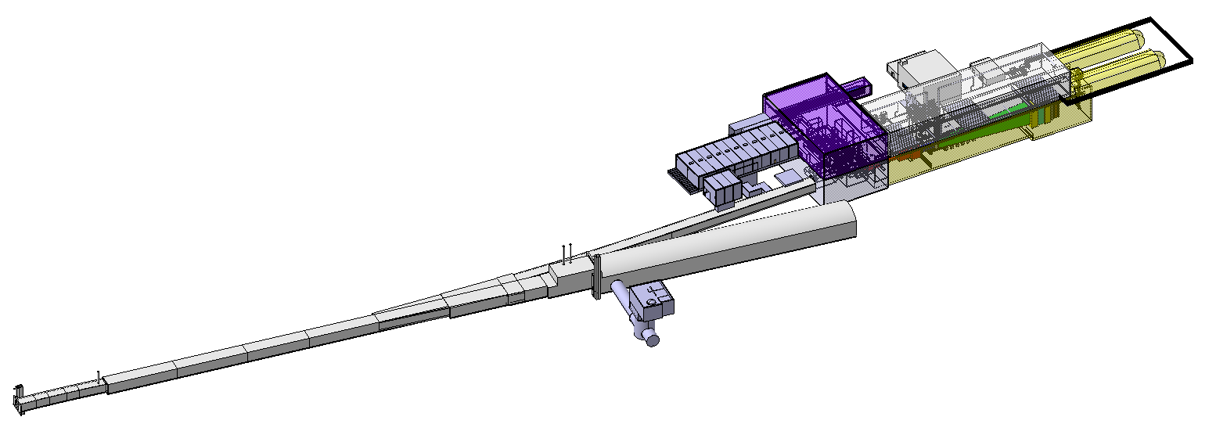
\includegraphics[width=0.9\columnwidth]{figs/BeamLine/2018_09_FacilityOverview.png}
\caption{}
\label{fig:FacilityOverview}
\end{figure}

\begin{figure}[th]
\centering
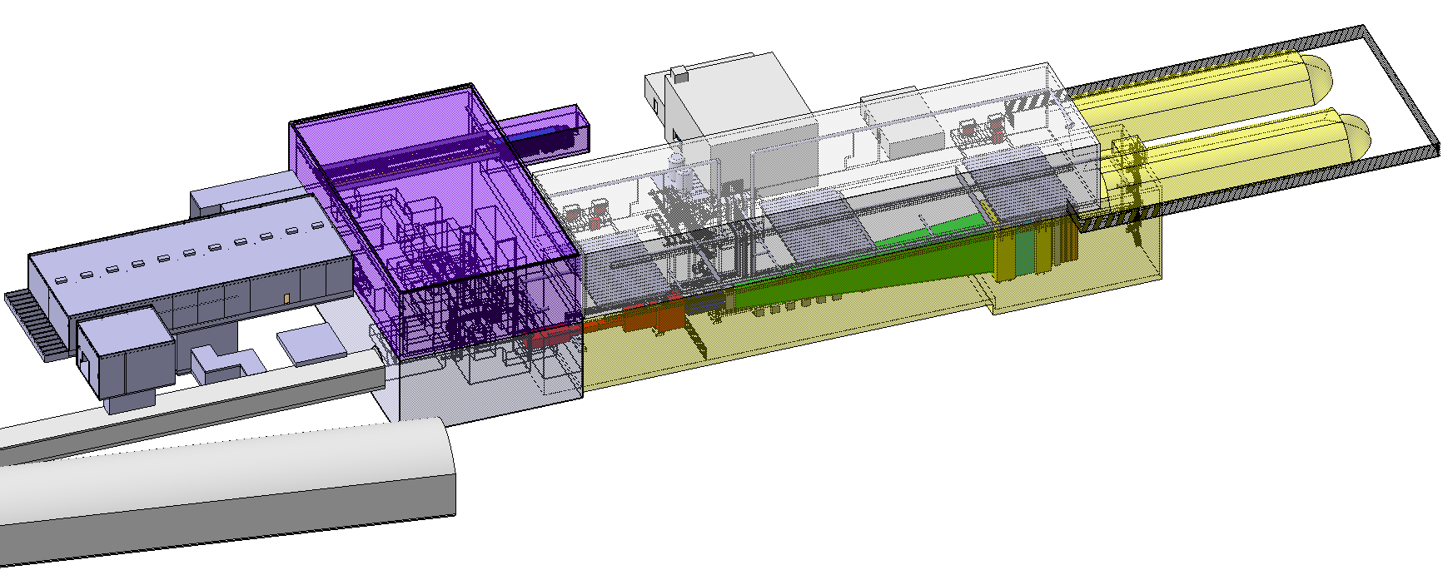
\includegraphics[width=0.9\columnwidth]{figs/BeamLine/2018_09_ExperimentalAreaOverview.png}
\caption{}
\label{fig:ExperimentalAreaOverview}
\end{figure}





\section{Potential siting of a search for Lepton Flavour Violation experiment}

(Pictures from presentation at BDF WG)

Motivation (yield)

From the beam optics point of view, several locations can provide the required beam conditions 
and the beam drift space to accommodate the detector along the new $200~m$ transfer line between 
the TDC2 switch yard cavern and the BDF target station without affecting the location of the BDF 
experimental area and without significant changes to the configuration of the beam line. The 
choice is instead driven by considerations related to the civil engineering in the vicinity of 
the existing installations, radiological protection, and to access and transport requirements 
above ground and underground.  Lateral space is required on both sides for shielding in order 
to limit the radiation exposure of the surrounding underground area to levels typical for the 
rest of the beam line.

The preferred location under study is situated $60~m$ upstream of the BDF target bunker. An 
access and service complex for the transfer line is already foreseen at this location. It would 
be extended and reconfigured to include a bypass tunnel, the detector bunker, service cavern 
and the required surface complex. 

By a modest reconfiguration of the existing beam elements, the location provides a beam spot of 
$\sigma_x=4.4~mm ~\times \sigma_y=1.1~mm$ and a drift space of $20~m$ to implement the detector 
and the shielding. A compensator magnet is foreseen to allow the experimental dipole magnet and 
the need to swap polarity. The downstream dilution system which is required to sweep the beam 
in a circle on the BDF target to dilute the beam power will have to be twice as strong in this 
configuration.

A first check of the characteristics of the proposed target configuration and beam induced 
effects on the material has revealed no showstopper. The target and the silicon-pixel detector 
will share a common closed volume containing an inert gas in circulation to prevent radiation 
induced corrosion and to ensure external cooling of the target and the detector.

A preliminary FLUKA study of the radiological aspects has been performed. It confirms that the 
radiation environment will be very challenging for the detectors. Remote handling will be 
required to move the detectors out of their data taking position into an adjacent service cavern 
for interventions. A shielding wall will separate the service cavern from the detector bunker 
during operation. No access is allowed underground during operation. An important challenge 
concerns preventing irradiation of the downstream beam elements due to radiation leakage through 
the whole in the shielding for the beam line.

A preliminary check of the surrounding environment shows no problems with respect to 
environmental limits or fluxes in neighbouring underground areas at the North Area, but this 
requires further studies. The additional flux of muons and neutrinos which enter the SHiP 
experiment will be studied as soon as the TauFV experimental configuration reaches more maturity.




%%%%%%%%%%%%%%%%%%%%%%%%%%%%%%%%%%%%%%%%%

%Since CERN currently has no experimental facility which is compatible with the full potential of the SPS, SHiP requires a new facility. CERN's North Area has a large space next to the SPS beam transfer lines which is largely free of structures and 
%underground galleries, and is entirely located on the current CERN territory. The proposed implementation is based on minimal modification to the SPS complex and maximum use of the existing beam lines. The design foresees space for future extensions.


% SHiP uses a target of 12 interaction lengths of molybdenum-tungsten 
% which has been designed to cope with % the large beam power and which 
% maximize the production % of charm and beauty hadrons, and the 
% production and % interactions of photons, while minimizing the production 
% of neutrinos from pion and kaon decays. The infrastructure complex to 
% house the proton target with the associated services and remote handling, 
% and which is fully compatible with the radiation protection and 
% environmental considerations, has been taken through an advanced feasibility 
% study.
%% KP detail i think...
%%A new type of beam splitter magnet allows switching the beam to a short new transfer line to the SHiP 
% experimental facility at the top of the TT20 transfer line, while maintaining operational all the current experimental facilities at the CERN North Area.






%The SHiP experiment incorporates two complementary apparatuses. The detector system immediately downstream of the muon shield is optimized for both recoil signatures of hidden sector particle scattering and for neutrino physics. It is based on an emulsion system interleaved with an electronic tracking system and high-density $\nu$-target layers in a magnetic field. The detector $\nu$-target mass totals ${\cal{O}}(10)~tonnes$. The emulsion spectrometer is followed by a muon identification system. This also acts as a tagger for interactions in the muon filters which may produce long-lived neutral mesons entering the downstream decay volume and whose decay may mimic signal events.
%The second detector system aims at measuring the decays of Hidden Sector particles to fully reconstructible final states as well as partially reconstructible final states that involve neutrinos. The spectrometer is designed to accurately reconstruct the decay vertex, the mass, and the impact parameter of the hidden particle trajectory at the proton target. A set of calorimeters and muon stations provide particle identification. %The system is optimized to as many final states as possible in order to be sensitive to, and discriminate between, a very wide range of models. 
%A dedicated timing detector with $\leq100~\ps$ resolution provides a measure of coincidence in order to reject combinatorial backgrounds. The decay volume is surrounded by background taggers to tag neutrino and muon interactions in the vacuum vessel walls and in the surrounding infrastructure.  %which may produce long-lived neutral SM particles, such as $K_L$ etc.

%The detector consists of a 50 m long decay volume followed by a large spectrometer with a rectangular acceptance of 5 m in width and 10 m in height. In order to suppress the background from neutrinos interacting in the fiducial volume, it is maintained at a pressure of ${\cal{O}}(10^{-3})~bar$. The spectrometer is designed to accurately reconstruct the decay vertex, the mass, and the impact parameter of the hidden particle trajectory at the proton target. A set of calorimeters and muon stations provide particle identification. The system is optimized to as many final states as possible in order to be sensitive to, and discriminate between, a very wide range of models. A dedicated timing detector with $100~ps$ resolution provides a measure of coincidence in order to reject combinatorial backgrounds. The decay volume is surrounded by background taggers to tag neutrino and muon inelastic scattering in the vacuum vessel walls which may produce long-lived neutral SM particles, such as $K_L$ etc.

% The muon shield and the SHiP detectors are housed in an underground hall $120~m$ in length and $20~m$
% width, at a depth of $\sim15~m$. 
% The proposed implementation of the SHiP experimental facility is based on minimal modification to the % SPS complex and maximum use of the existing accelerator and beam lines. All civil engineering works 
% are fully located within existing CERN land on the Prevessin site.
%%%%%%%%%%%%%%%%%%%%%%%%%%%%%%%%%%%%%%%%%




%\section{Simulation}
\label{sec:simulation}


\section{Changes since Technical Proposal}
\subsection{Simulation}
\label{sec:simulation}
The simulation of the proton on fixed-target collisions is done in two steps, primary proton-proton or proton-neutron collisions are simulated using Pythia8, and the particles produced are transported through the experimental setup using Geant4. Some important sources of background muons are not generated by default in Geant4, like decays of light vector mesons to $\mu^+\mu^-$, $\gamma$-conversions to $\mu^+\mu^-$, positron annihilation to $\mu^+\mu^-$. These are all rare processes, but can potentially cause background in the detector due to not being diverted by the active muon shield because of high momentum or wrong charge of the muon. Their rate had been increased artificially in the simulation by a factor $100$ to simulate enough statistics to study these events in detail.

% add figure of muon leaving hadron absorber as function of p/pt, with different sources, or table

For the heavy quark production, a procedure had been put in place to simulate also charm and beauty hadron production by the products of the primary proton nucleon collision~\cite{cascade}. % myBiblio.bib
This increases the yield expectation compared to the prediction in the Technical Proposal by a factor of $2.6$($1.9$) for  $1$($3$) $GeV/c$ HNLs in the acceptance.

Simulated in total $65$ billion protons on target with an energy cut for transporting particles after the hadron absorber of $10$ GeV, and $1.8$ billion protons on target with an energy cut of $1$GeV. The samples produced with charm and beauty hadrons correspond to about $100$ billion protons on target.

\begin{figure}[h]
\centering
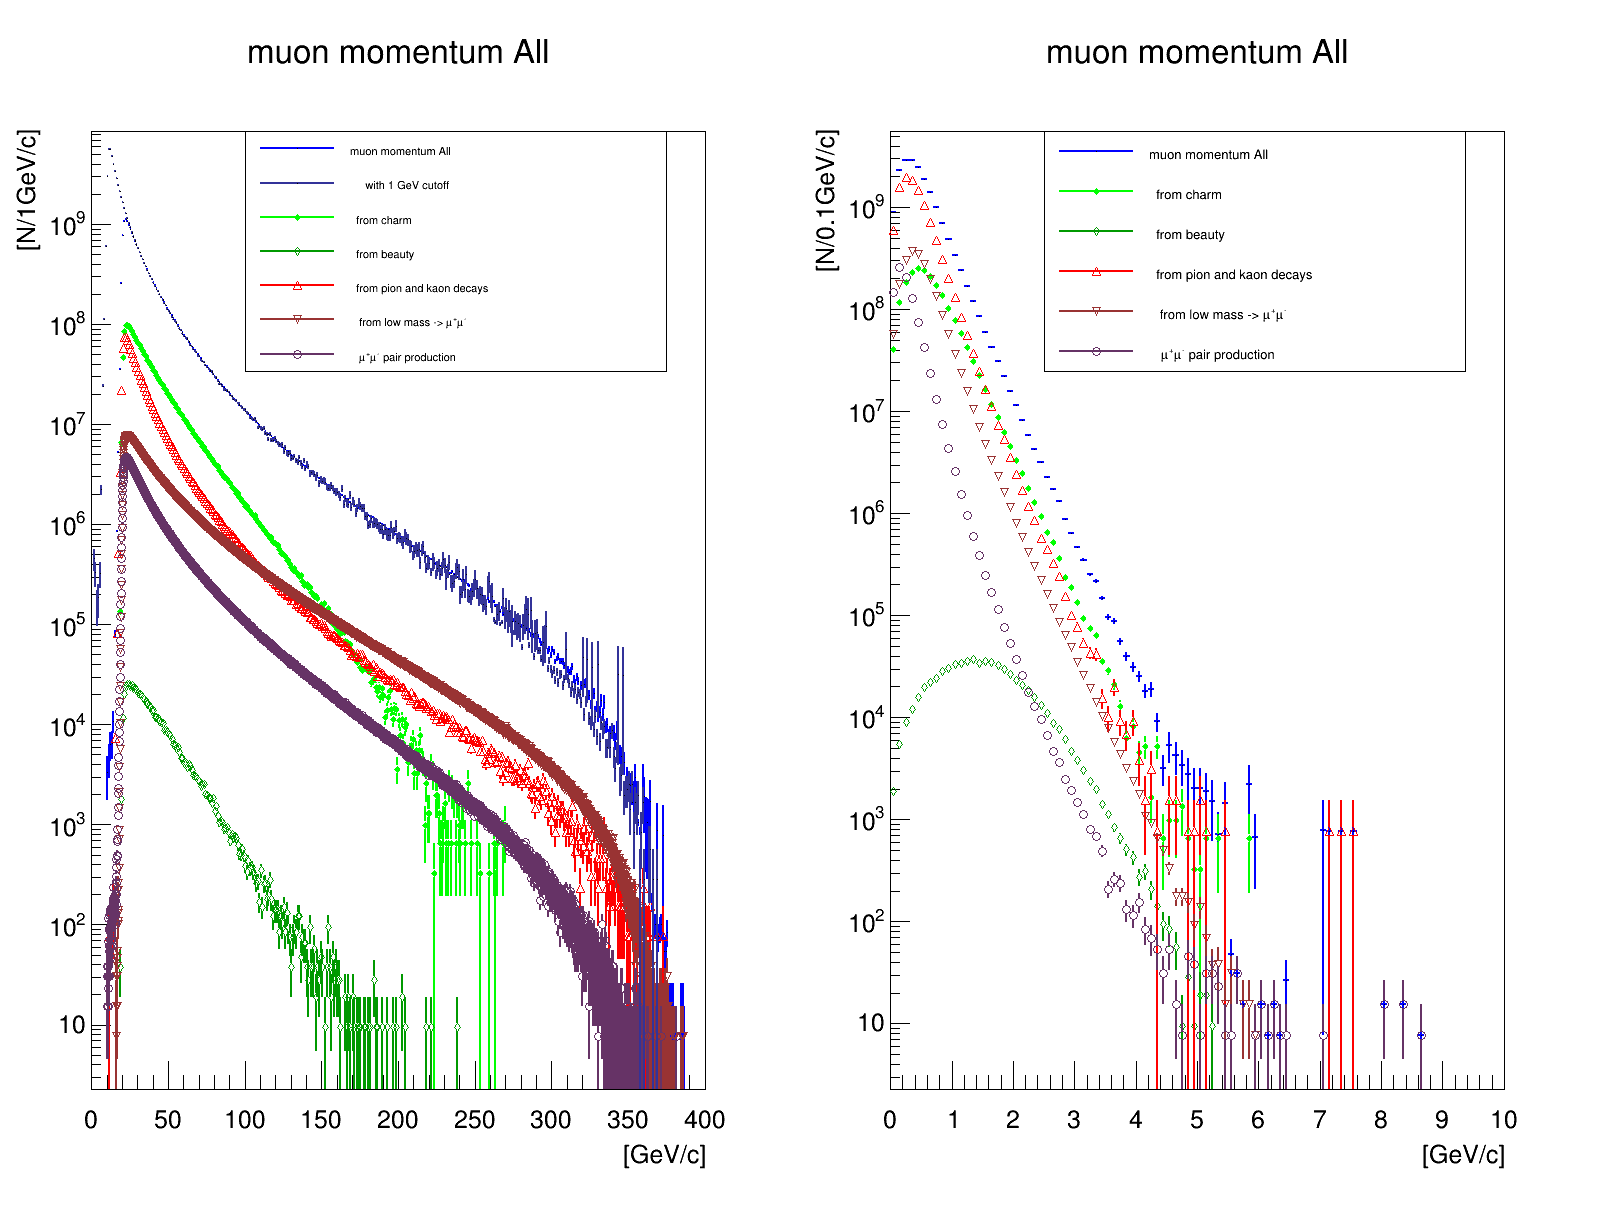
\includegraphics[width=8cm]{figs/muonMom.png}
\caption{Momentum distributions of muons leaving the hadron absorber, total momentum (left) and transverse momentum(right). Different contributions are shown. The rates are normalized to one spill ($5\times 10^{13} $) protons on target.}
\label{fig:muonMom}
\end{figure}

\begin{figure}[h]
\centering
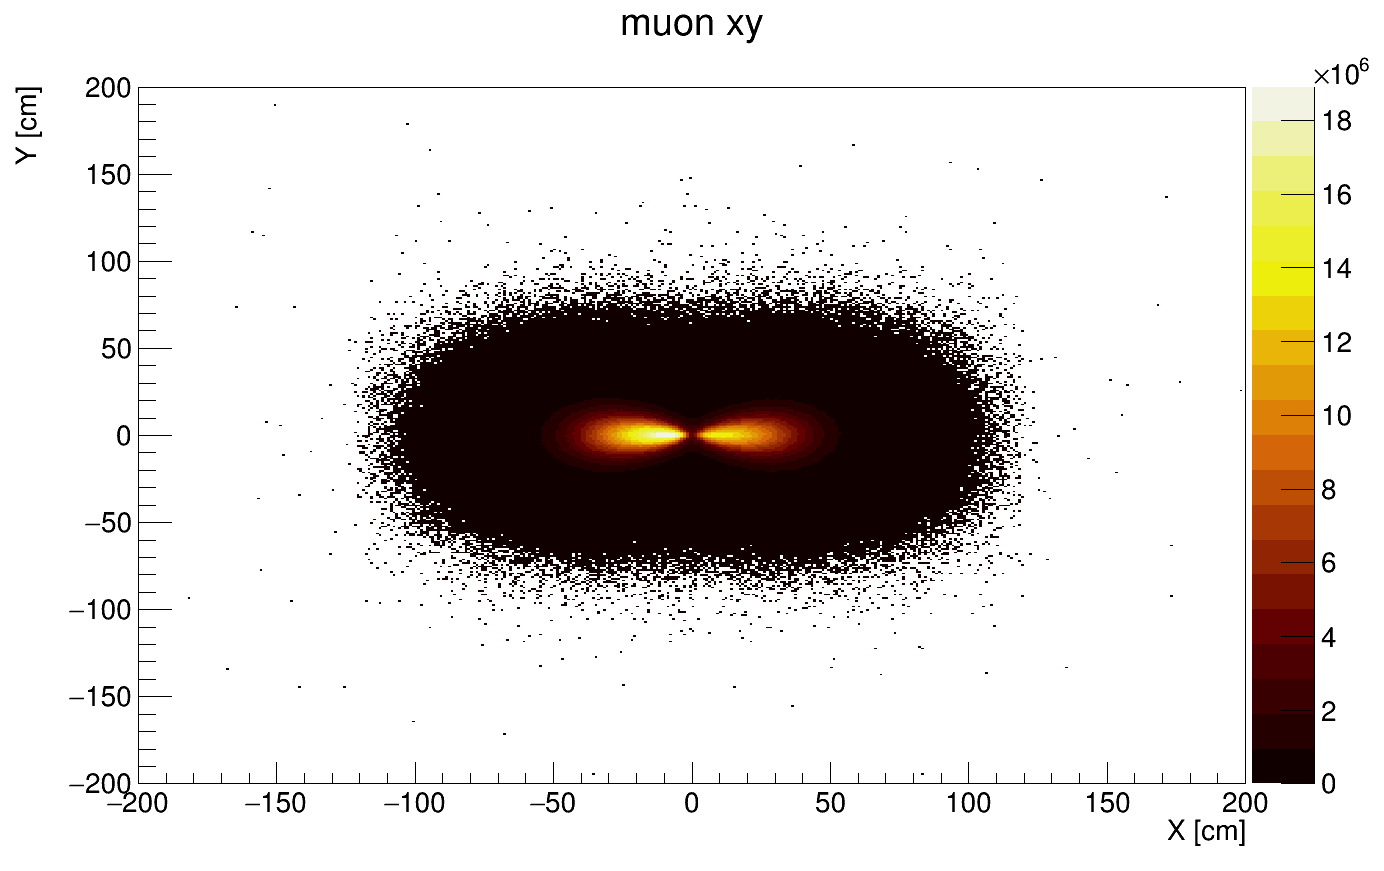
\includegraphics[width=8cm]{figs/muonXY.png}
\caption{Position of muons leaving the magnetized hadron absorber.}
\label{fig:muonXY.png}
\end{figure}


\begin{figure}[h]
\centering
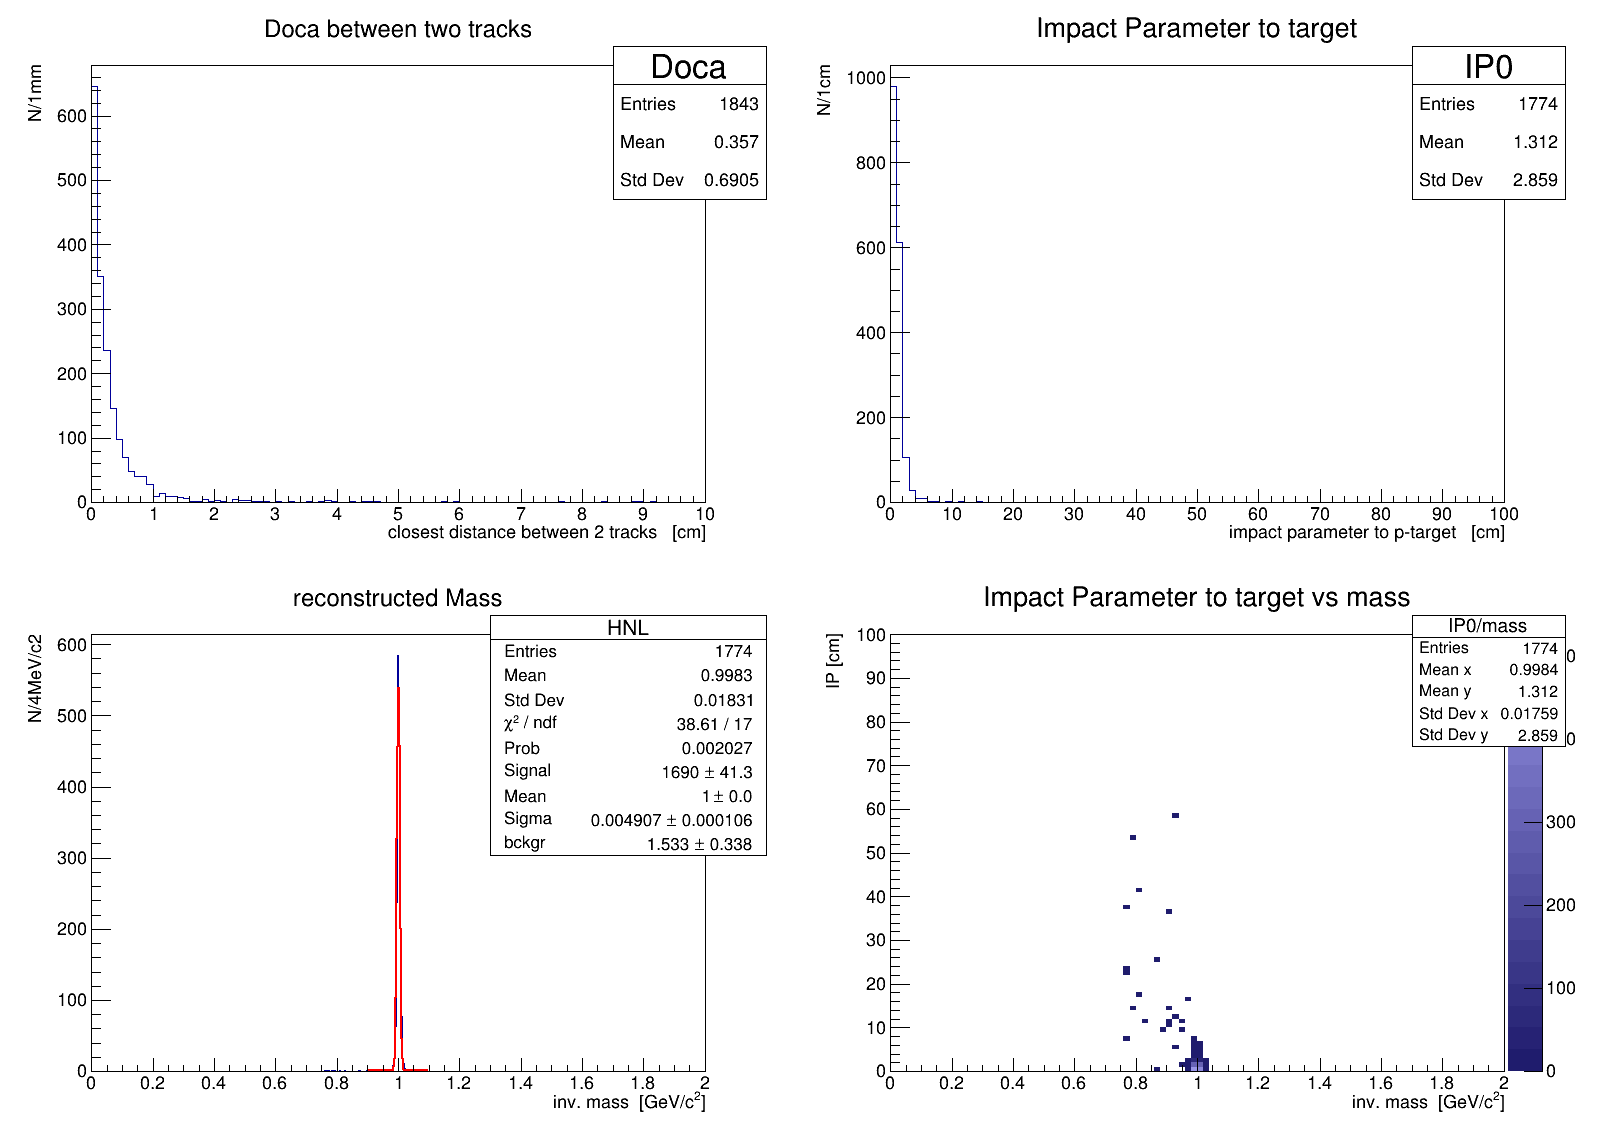
\includegraphics[width=8cm]{figs/mupiperformance.png}
\caption{Reconstruction of $HNL\rightarrow \mu^-\pi^+$.}
\label{fig:signalpimu.png}
\end{figure}

\begin{figure}[h]
\centering
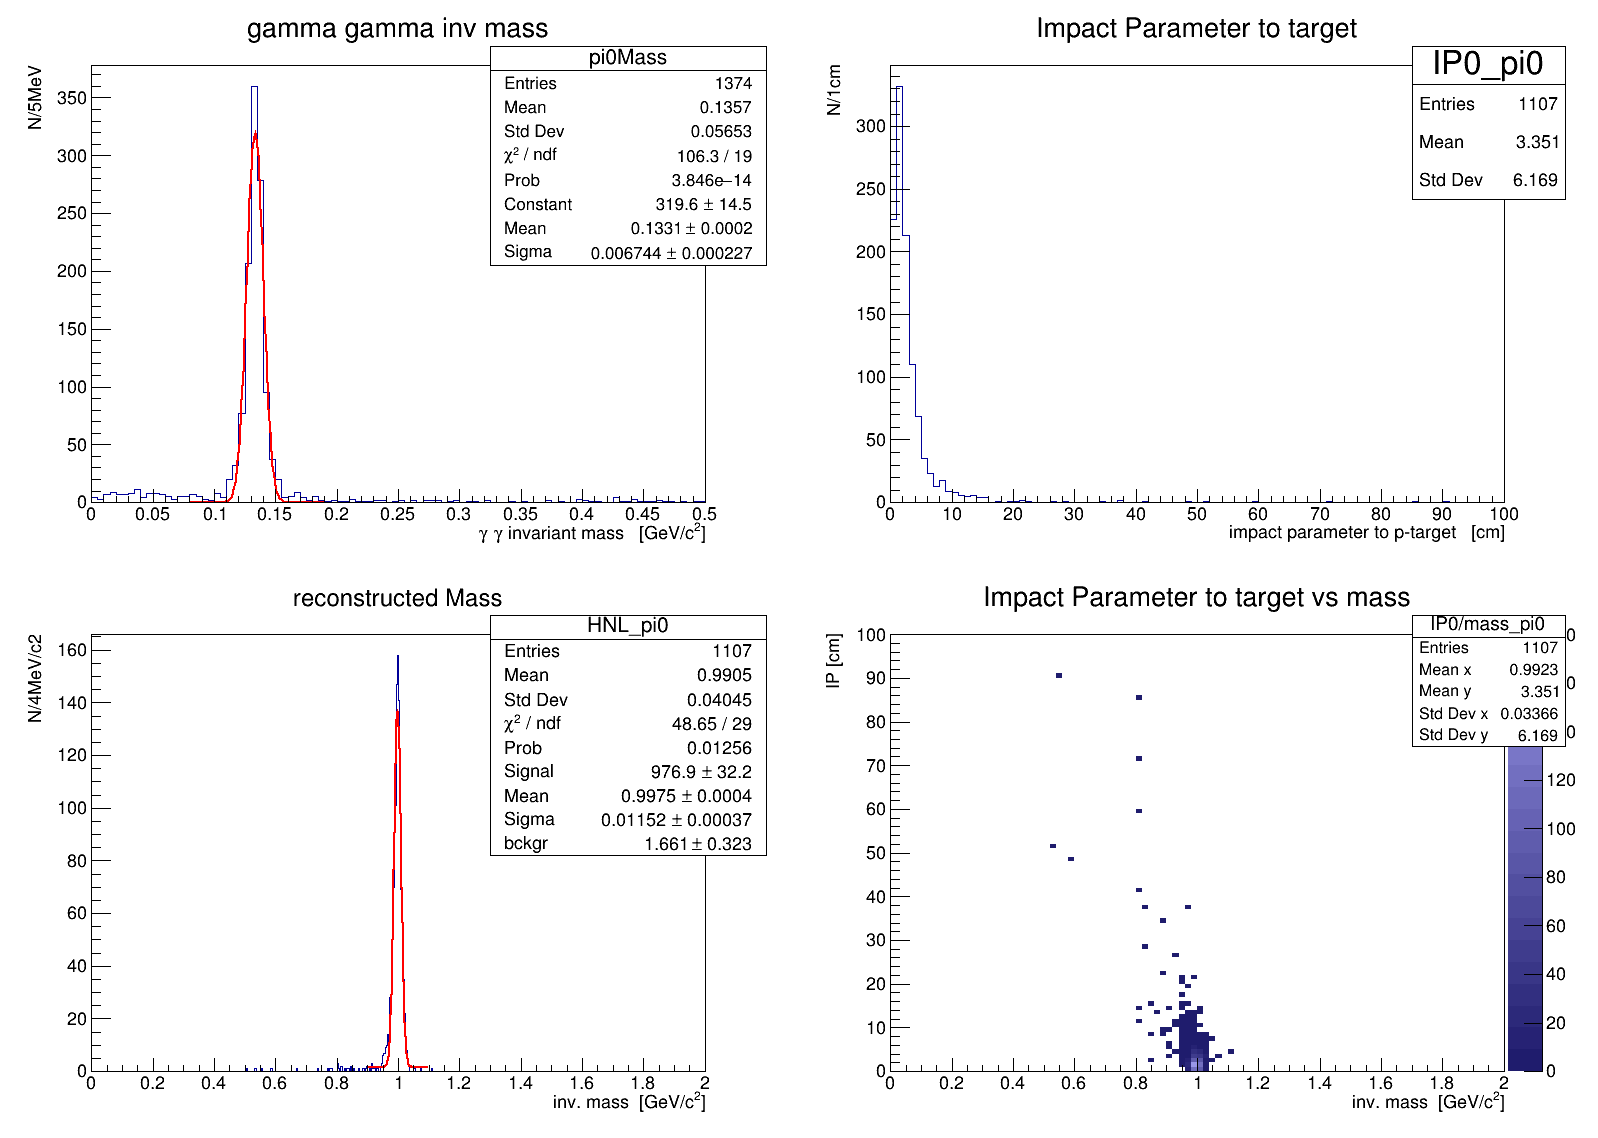
\includegraphics[width=8cm]{figs/murhoperformance.png}
\caption{Reconstruction of $HNL\rightarrow \mu^- \rho^+(\rightarrow\pi^+\pi^0(\rightarrow\gamma\gamma))$.}
\label{fig:signalrhomu.png}
\end{figure}

\begin{figure}[h]
\centering
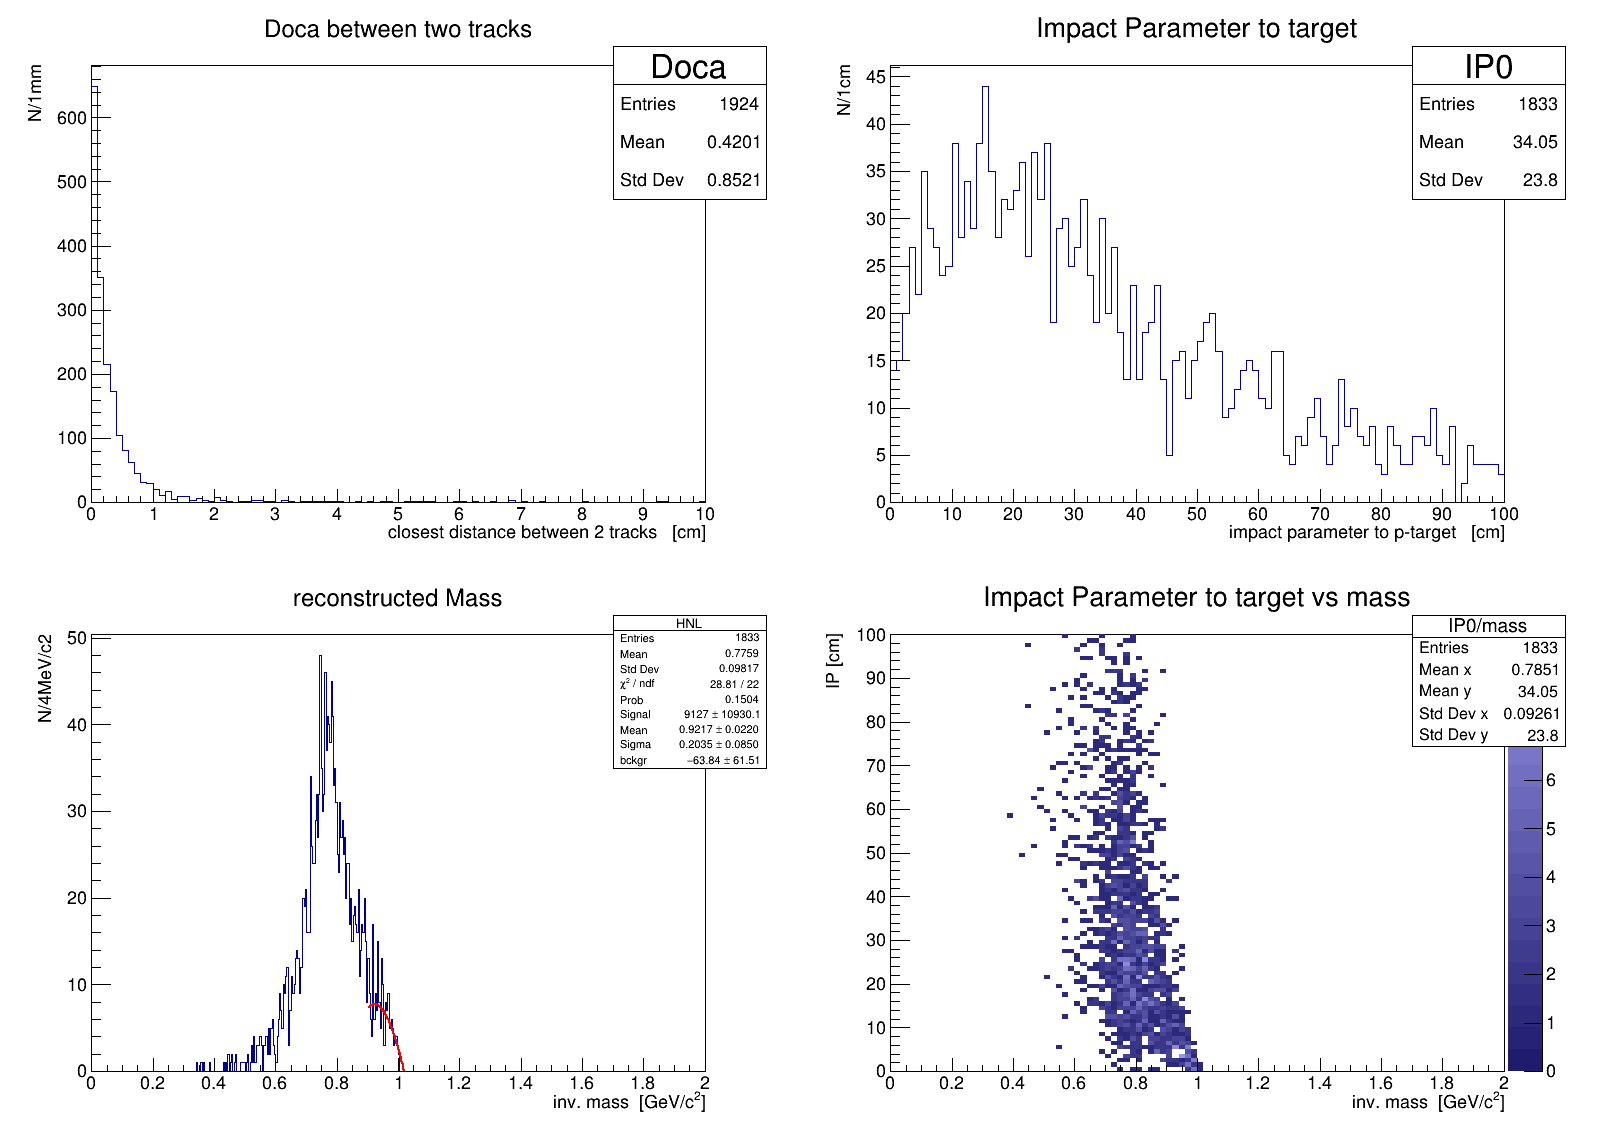
\includegraphics[width=8cm]{figs/numuperformance.png}
\caption{Reconstruction of $HNL\rightarrow \nu\rho^0(\rightarrow\pi^+\pi^-$.}
\label{fig:signalnumurho0.png}
\end{figure}

\begin{figure}[h]
\centering
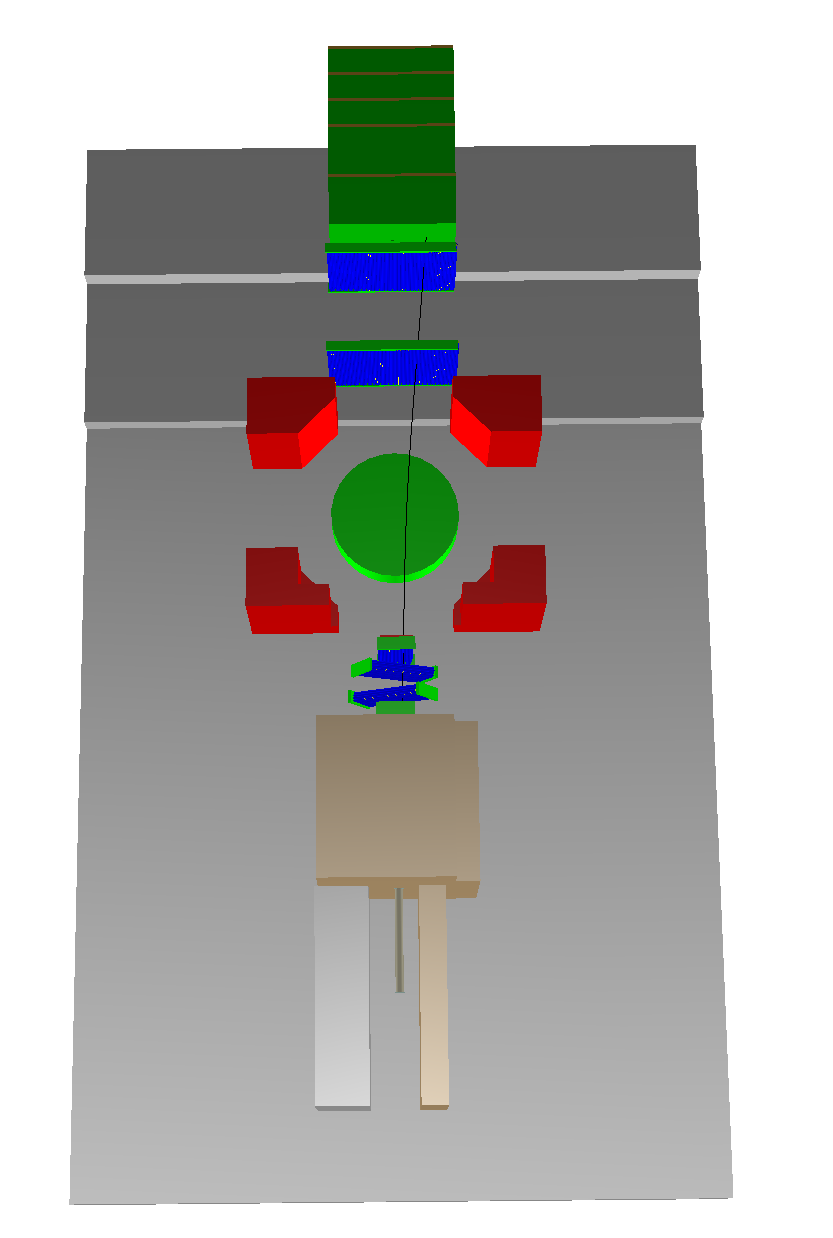
\includegraphics[width=8cm]{figs/muflux-setup-withTrack.png}
\caption{Muflux testbeam setup with a track reconstructed using FairShip. }
\label{fig:eventDisplay.png}
\end{figure}


Cross checks of simulation with data:
\begin{itemize}
  \item Studying Multiple Scattering with GEANT4 v10.3.2, The multiple scattering as implemented in the GEANT4 version currently employed in the FairShip simulation is compared to existing data and other models.
CERN-SHiP-NOTE-2017-003, see Fig.\ref{fig:data}. Good agreement is found.
  \item Comparing catastrophic energy loss of muons in a liquid krypton calorimeter (NA62, https://indico.in2p3.fr/event/420/contributions/29860/attachments/24033/29479/moriond.pdf ) with Geant4.  The Geant4 setup consists of $125$cm thick block of liquid krypton.
  Muons are shot on the block, and the energy deposited in the block is summed up.  (The muon critical energy for which radiative and ionization energy loss rates are equal is about $280$ GeV/c in liquid krypton and $350$ GeV/c for iron, D.E. Groom, N.V. Mokhov, and S.I. Striganov, “Muon stopping-power and range tables: 10 MeV–100 TeV,” Atomic Data and Nuclear Data Tables 78, 183–356 (2001).)  The mean energy deposited in the liquid krypton does not agree well with the mean energy loss expected for muons (right plot).
  \item A specific experiment had been setup in the CERN North Area to measure directly the rate and momentum of muons of $400$ protons impinging on a replica of the SHiP target after a $xx$m.
\end{itemize}


\begin{figure}[htb]
\begin{center}
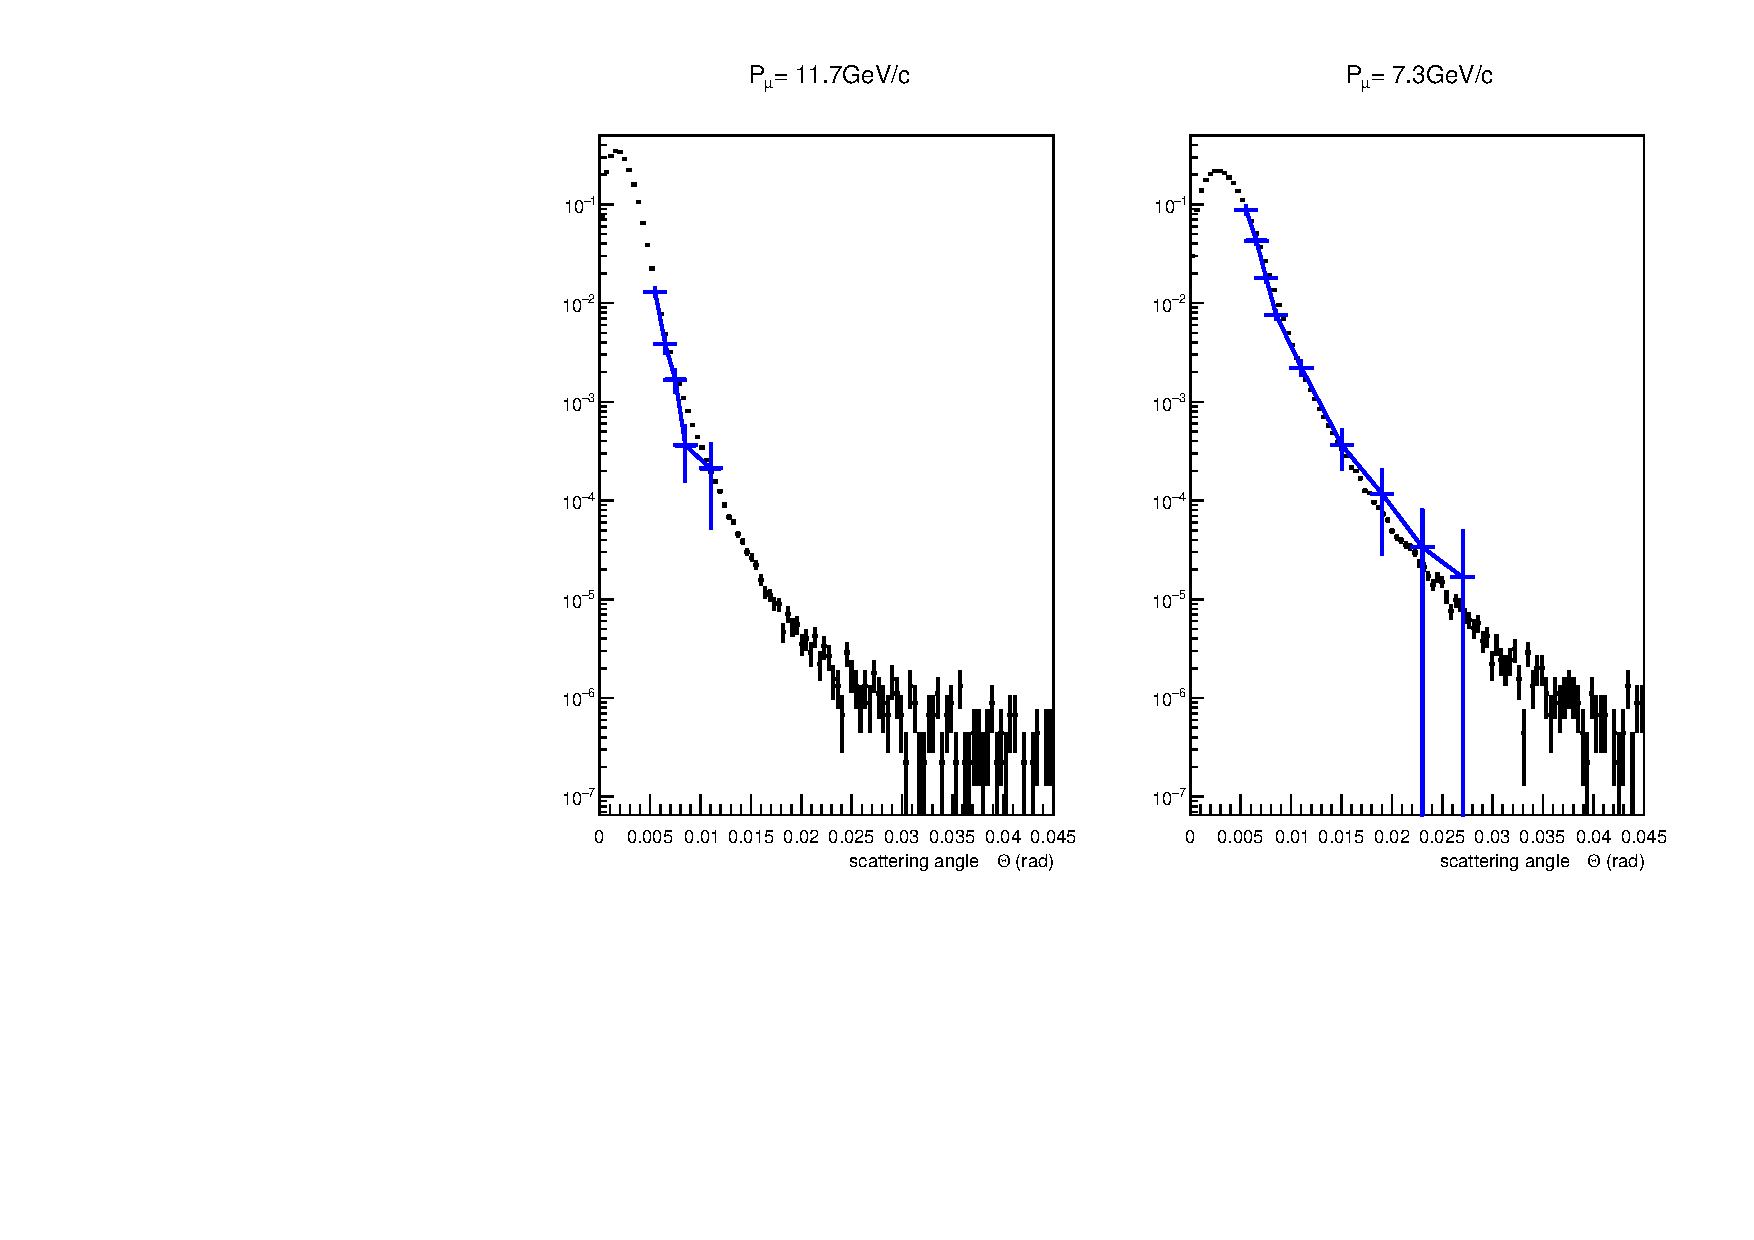
\includegraphics[width=0.8\linewidth]{figs/dataMSC.pdf}
\caption{ Comparison of the GEANT4 Monte Carlo simulation to the 11.7 GeV/c data-set (left) and 7.3 GeV/c data-set (right). Blue points are the measurements of \cite{Akimenko:1984qw}, black points are from the FairShip simulation. }
\label{fig:data}
\end{center}
\end{figure}

\begin{figure}[htb]
\begin{center}
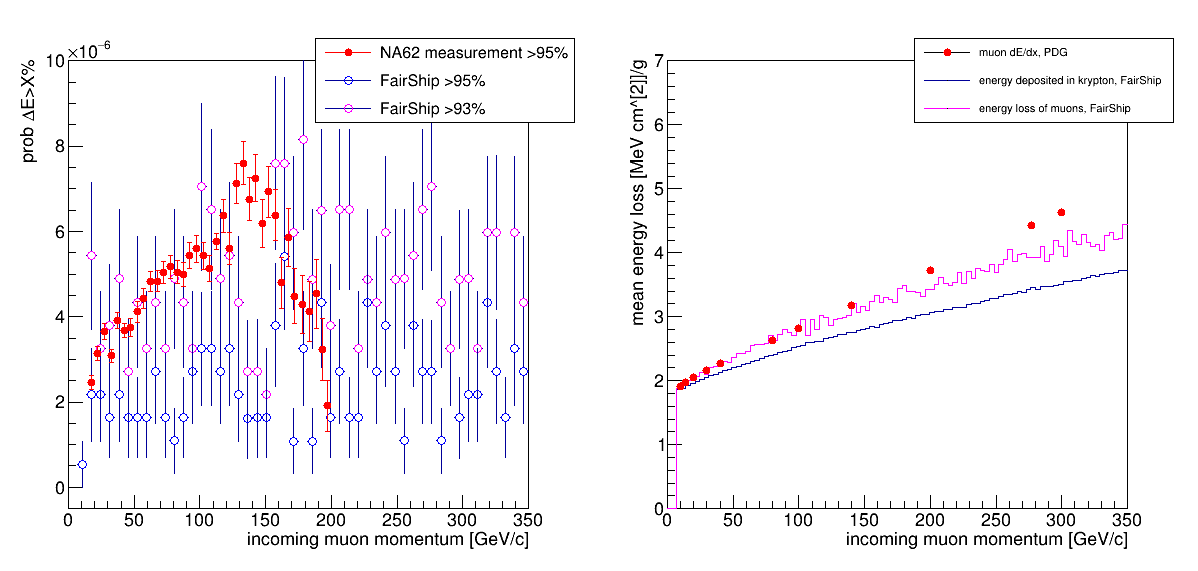
\includegraphics[width=0.8\linewidth]{figs/catastrophicEnergyLoss.png}
\caption{ Left: Probability that a muon releases in the liquid krypton calorimeter more than 95\% of its energy as a function of the muon momentum in GeV/c, red points NA62 measurements, blue points FairShip simulation, magenta points FairShip with >93\%.
Right: mean energy loss as function of muon momentum. Note, energy deposited in krypton is less than the energy loss of a muon. At higher energies, mean energy loss is lower than expected.}
\label{fig:data}
\end{center}
\end{figure}

\subsection{Detector Setup}
\label{sec:detectors}
Strawtracker diameter increased from $1$cm to $2$cm to save readout channels, no effect on momentum / vertex resolution observed.
Same dimensions for all straw tracker stations. Support material added to simulation.

Moved to use realistic field maps for the spectrometer magnet (from OPERA simulation) and for the active muon shield, compared to using an analytic function for the bending field (no return field) and constant fields in the active muon shield. The latter changed the background from ? to ? (ask Oliver,

Active muon shield optimized for frustum detector setup

many changes to nu tau detector, described elsewhere. Takes over in addition task of upstream veto tagger.

straw veto tagger removed, vertex information enough to veto background of $K_S$ decays.

added second Ecal detector option, splitCal, which is under study. Removed HCal



\subsection{Reconstruction}
\label{sec:reconstruction}
different pattern recognition algorithm tested. Reconstruction of signal decays to two charged tracks and a pi0.





%\section{Scattering Spectrometer}
\label{sec:scatteringspectrometer}

\subsection{Detector layout}

\begin{itemize}
    \item Motivations for new design: dependence of neutrino flux from the radius, reduced area free from background muons 
    \item Description of \emph{One magnet} design (Figure \ref{fig:spectro_layout})
    \item \emph{One magnet} option VS \emph{Two magnets} option


\begin{figure}[htbp]
\centering
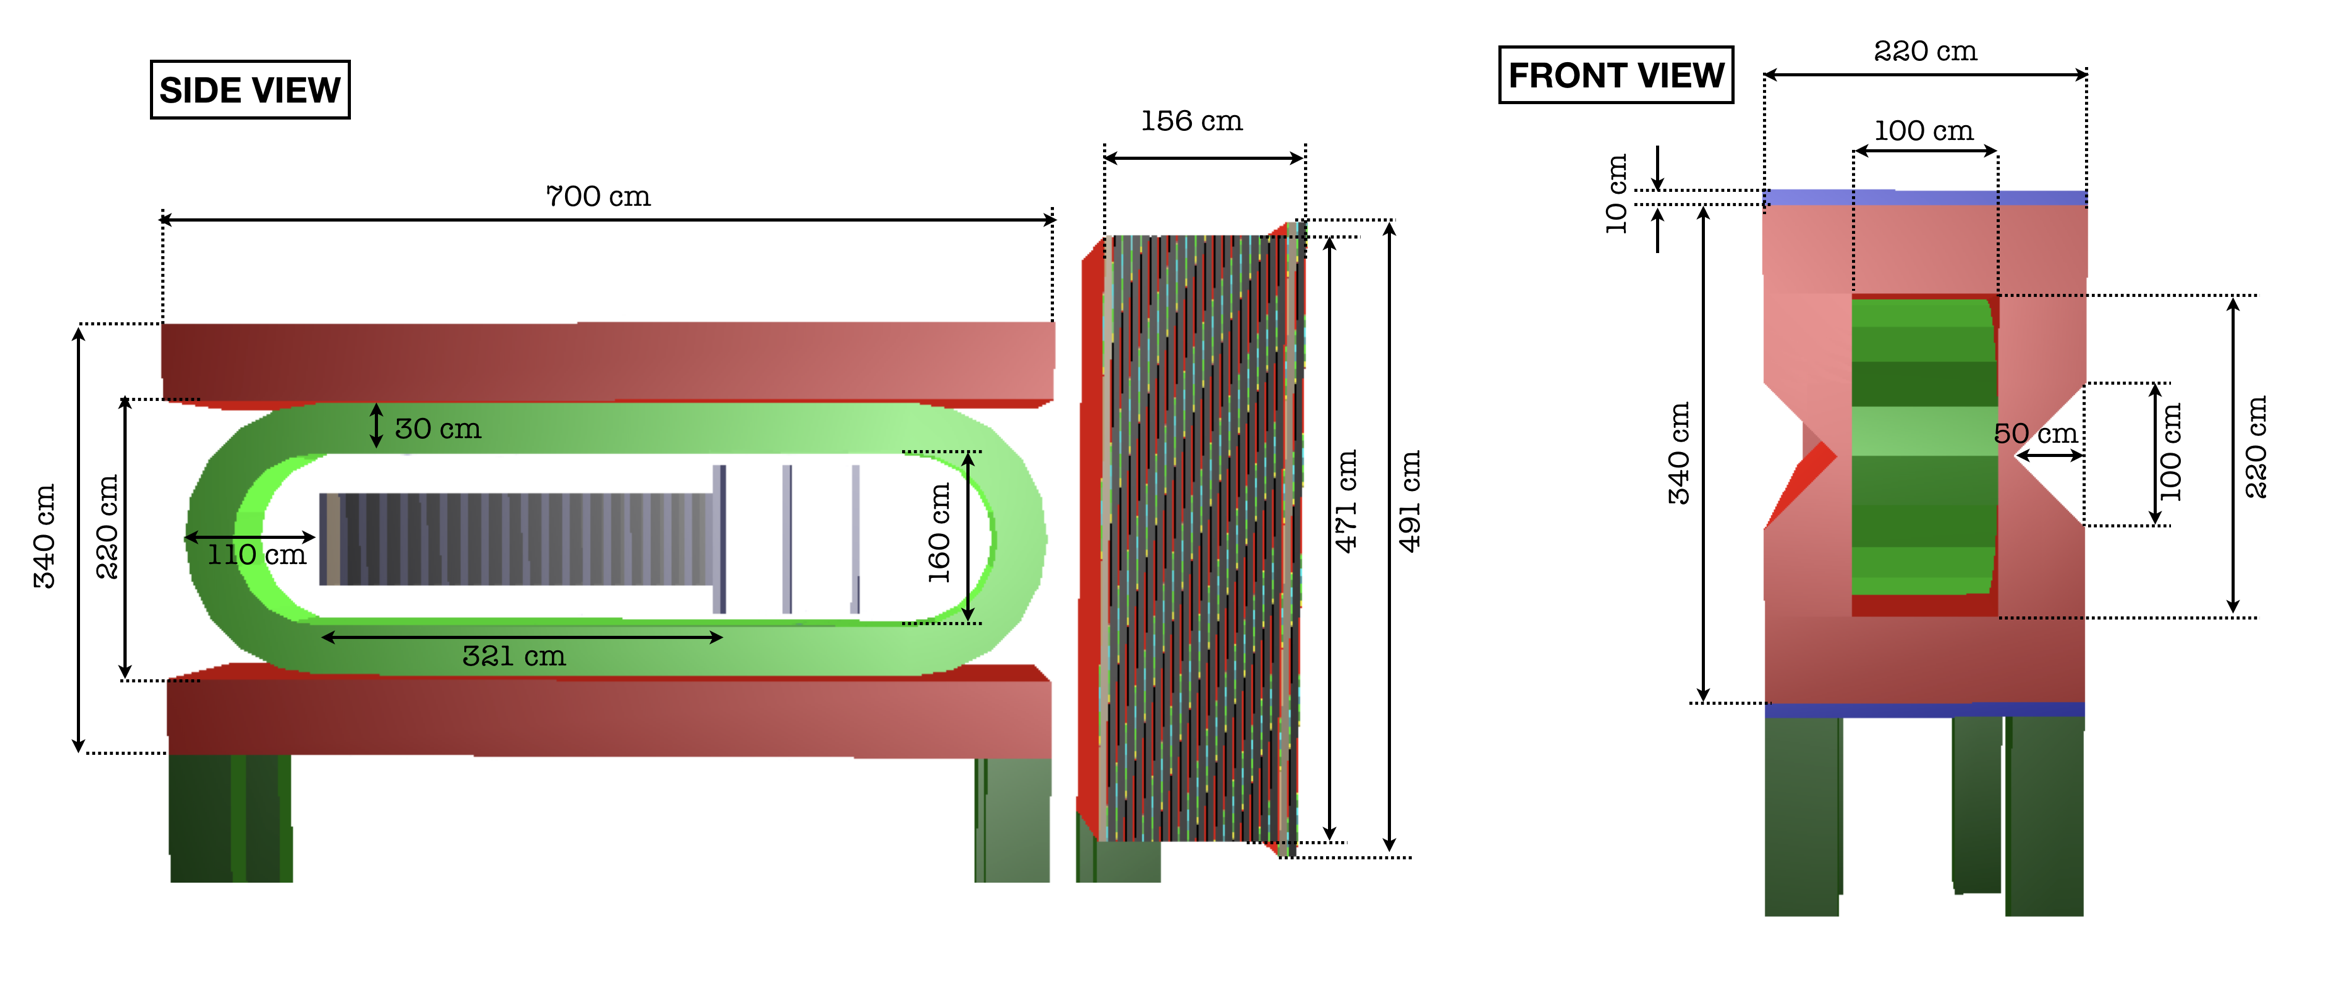
\includegraphics[scale=0.35]{figs/ScatteringSpectrometer/ScatteringSpectro.png}
\caption{Layout of the Scattering Spectrometer}
\label{fig:spectro_layout}
\end{figure}

\item Magnet design
 \begin{itemize}
 \item[$\circ$] Main constraints: inner volume and cross-section, 1.2 T uniform magnetic field, saturation field in iron, access to inner detector
 \item[$\circ$] Description of the magnet layout (Figure \ref{fig:magnet_layout})
 \end{itemize}
 

\begin{figure}[htbp]
\centering
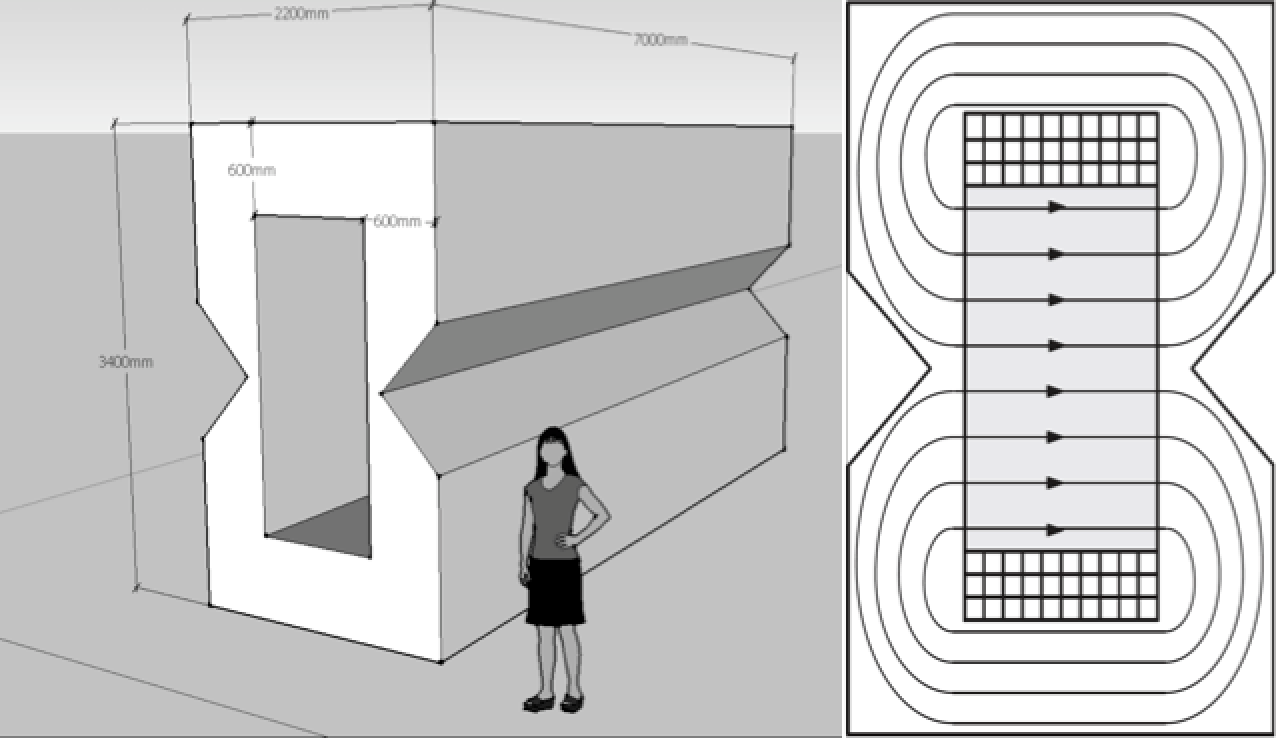
\includegraphics[scale=0.35]{figs/ScatteringSpectrometer/ScatteringSpectroMagnet.png}
\caption{Layout of the Scattering Spectrometer Magnet}
\label{fig:magnet_layout}
\end{figure}

\item Emulsion Target 
\begin{itemize}
    \item[$\circ$] Emulsion Cloud Chamber
    \item[$\circ$] Compact Emulsion Spectrometer: results from 2017 Test Beam
\end{itemize}

\item Target Trackers
\begin{itemize}
    \item[$\circ$] Requirements
    \item[$\circ$] Options under investigation: gas detectors (results from 2017 Test Beam), SciFi
\end{itemize}

\item Magnetic Spectrometer
\begin{itemize}
    \item[$\circ$] Requirements
    \item[$\circ$] Option under investigation: SciFi
\end{itemize}

\item Muon Filter
\begin{itemize}
    \item[$\circ$] Requirements
    \item[$\circ$] Detector layout
\end{itemize}

  \end{itemize}
  
\subsection{Neutrino detection}
\begin{itemize}
    \item Track reconstruction and primary vertex identification
    \item Decay search
    \item Charge measurement 
    \item Momentum measurement
    \item Particle identification in the Muon Filter
    \item Overall detection efficiency for different $\tau$ decay channels
\end{itemize}

\begin{figure}[htbp]
\centering
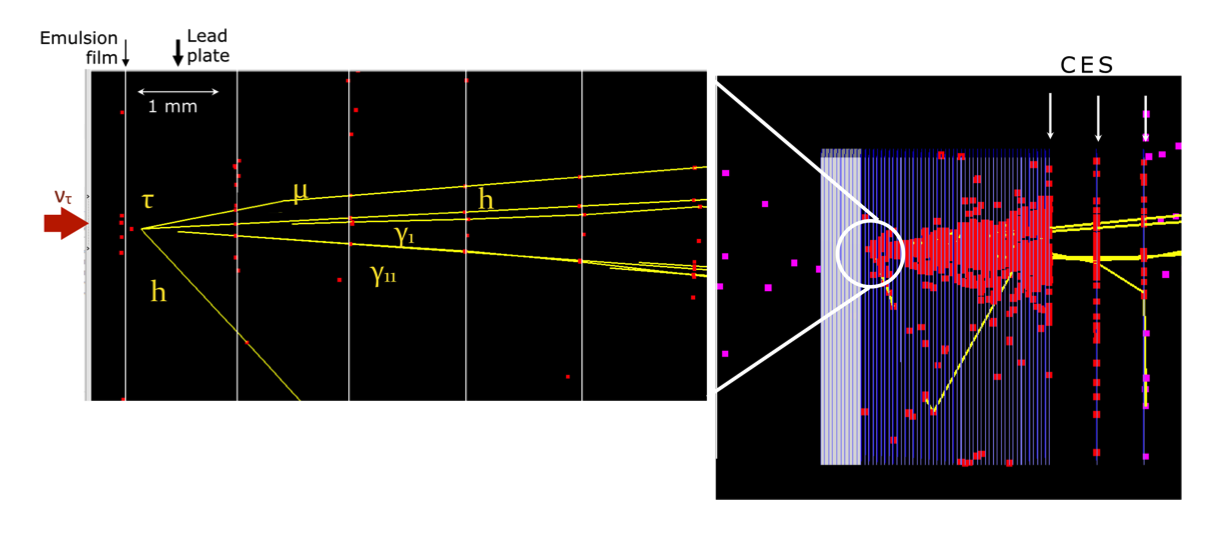
\includegraphics[scale=0.5]{figs/ScatteringSpectrometer/NeutrinoRecEmu.png}
\caption{$\nu_\tau$ interaction and subsequent $\tau \to \mu$ decay in the Emulsion Target.}
\label{fig:neutrino_rec_emu}
\end{figure}

\begin{figure}[htbp]
\centering
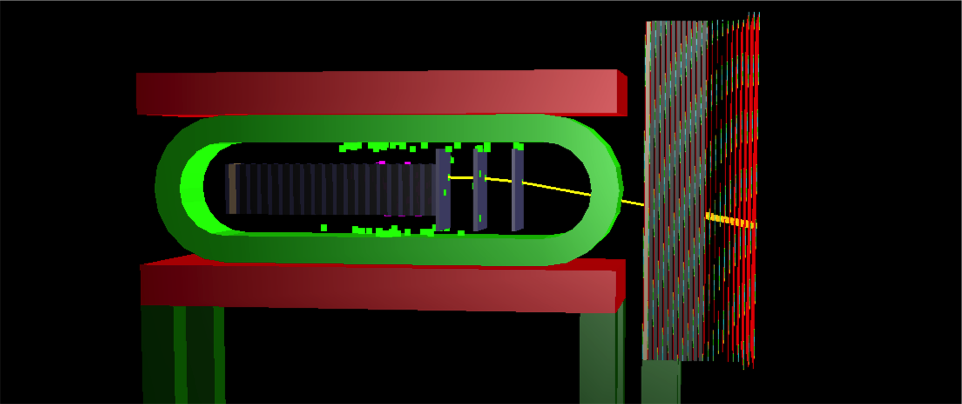
\includegraphics[scale=0.5]{figs/ScatteringSpectrometer/NeutrinoRecAll.png}
\caption{$\nu_\tau$ interaction and subsequent $\tau \to \mu$ decay in the Scattering Spectrometer.}
\label{fig:neutrino_rec_all}
\end{figure}

\subsection{Electromagnetic shower identification}
\begin{itemize}
    \item Pattern recognition (Figure \ref{fig:shower_id})
    \item Energy resolution (Figure \ref{fig:shower_res})
    \item Pointing accuracy 
\end{itemize}

\begin{figure}[htbp]
\centering
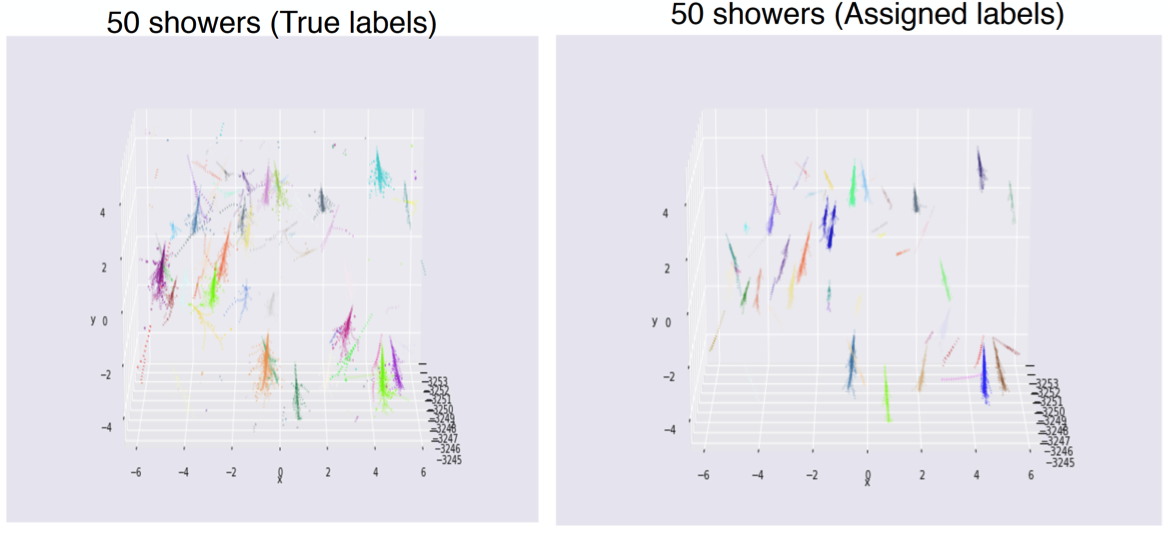
\includegraphics[scale=0.6]{figs/ScatteringSpectrometer/Showers.png}
\caption{Electromagnetic shower identification in the ECC.}
\label{fig:shower_id}
\end{figure}

\begin{figure}[htbp]
\centering
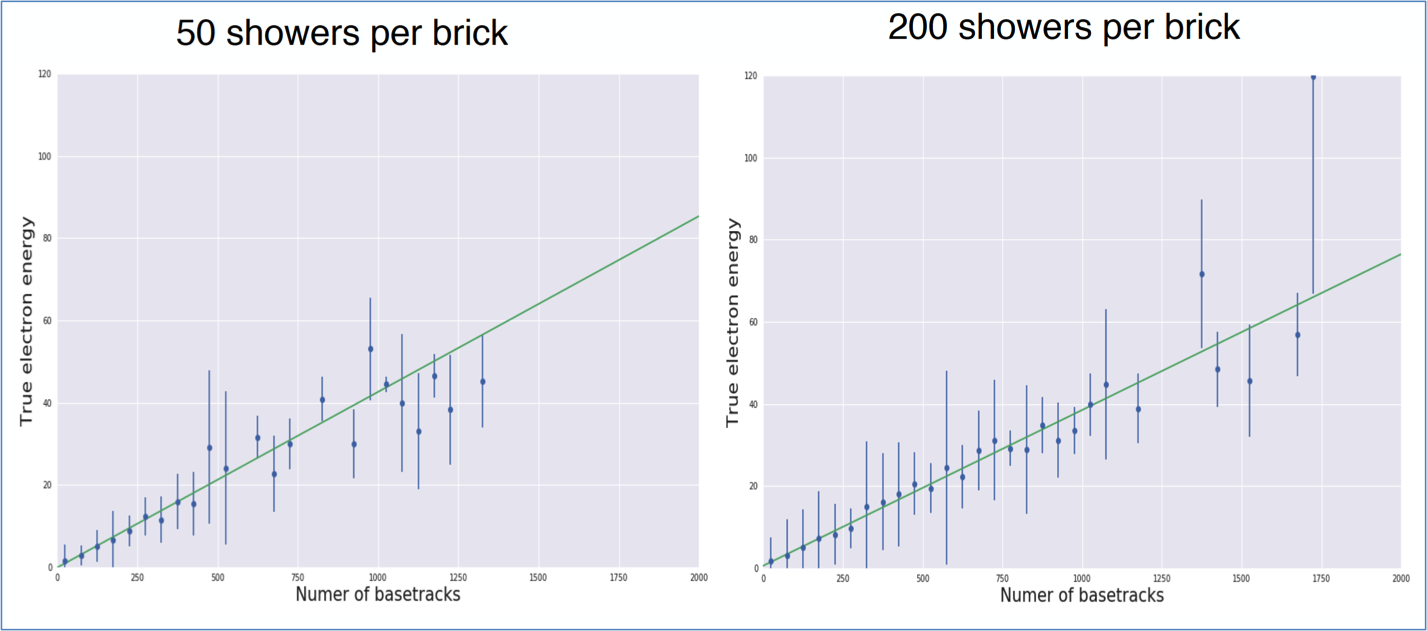
\includegraphics[scale=0.5]{figs/ScatteringSpectrometer/ShowersRes.png}
\caption{Energy resolution of electromagnetic showers in the ECC.}
\label{fig:shower_res}
\end{figure}

\subsection{Timing performances}

\subsection{Combined performances of TT and ECC/CES}


%\section{Decay Spectrometer}
\label{DecaySpectrometer}
\subsection{Overview of re-optimized Decay Spectrometer}

The SHiP Decay Spectrometer (DS) consists of large vacuum vessel, Surround Background Tagger (SBT), Main Spectrometer Tracker (ST), including a large spectrometer magnet with a total field integral of XX Tm, Timing Detector (TD), Calorimeter and downstream Muon systems.

DS has to perform precise measurements of tracks and photons originated from decay vertices of hidden particles in the decay volume, measure their momenta, and provide PID information. Moreover DS has to ensure a redundant background suppression using timing and tracking information from TD and SST, vetoing criteria from SBT, and PID by the calorimeter system and muon detector. 

This section describes the principal features and main parameters of the DS sub-detectors as implemented in the FairSHiP. The parameters have used in the simulation studies of the DS performance reported in section \ref{DSperformance}. Specific proof-of-principle tests of prototypes have been undertaken which demonstrate that the parameters listed can be achieved.

\noindent {\bf SBT}\\
\noindent
SBT detects charged particles either entering the vacuum vessel from outside, or produced in the inelastic interactions of muons and neutrinos inside the vacuum vessel walls. Compared to the TP there are currently two options of the SBT under consideration: a new plastic scintillator (PS-SBT) option, and the liquid scintillator (LS) detector (LS-SBT) which remains the baseline with the LS of linear alkybenzene (LAB) and 2.0 g/l diphenyl-oxazole (PPO) as the fluorescent.

The LS-SBT is sub-divided in individual cells integrated to the support structure of the vacuum vessel. Accordingly, the cell size is 80 cm in the longitudinal direction and typically O(120 cm) in the transverse direction, depending also on its z-position. The thickness of the LS layer, surrounding the side walls of the complete decay vessel up to XX cm and enclosed by a YY cm thick outer steel wall, is 30 cm. Due to the conical shape of the decay vessel the LS volume of O(243 m$^3$) is significantly reduced compared to the TP.  This allowed to increase the PPO concentration from 1.5 g/l quoted in the TP without any increase in price for the LS.
%
\begin{figure}[h]
\centering
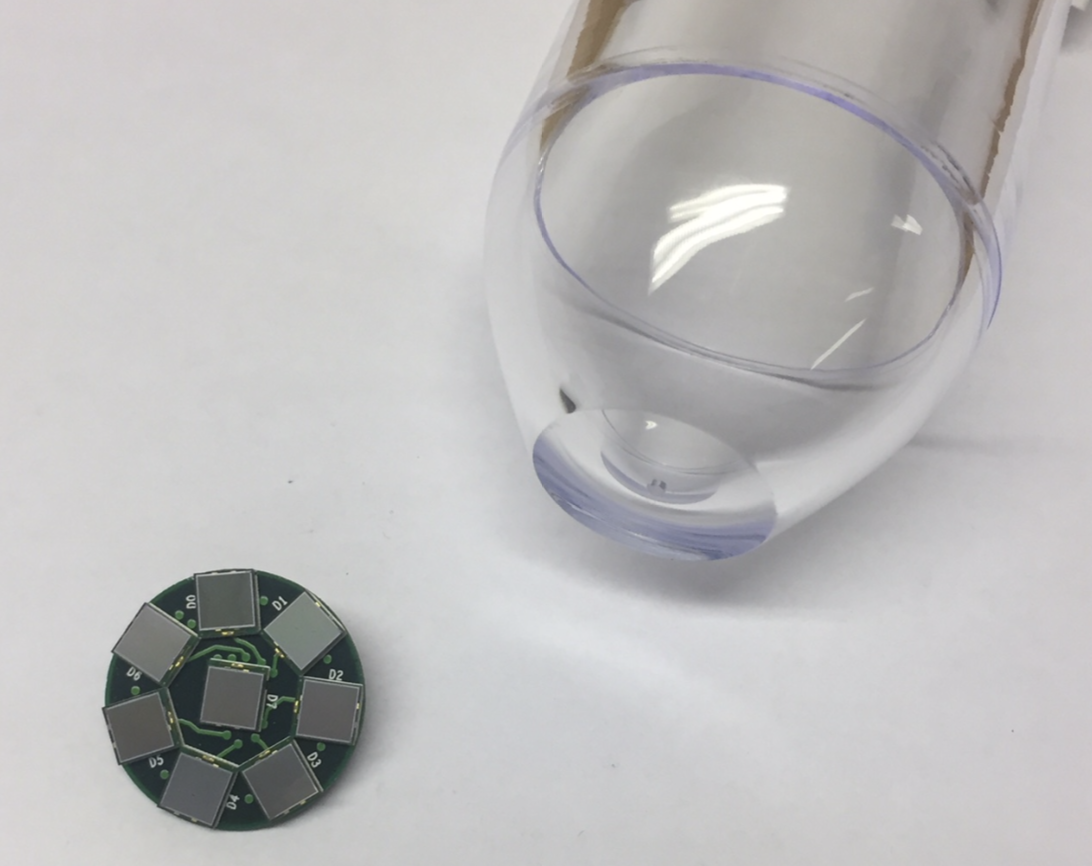
\includegraphics[width=0.35\columnwidth]{figs/DecaySpectrometer/WOM.png}
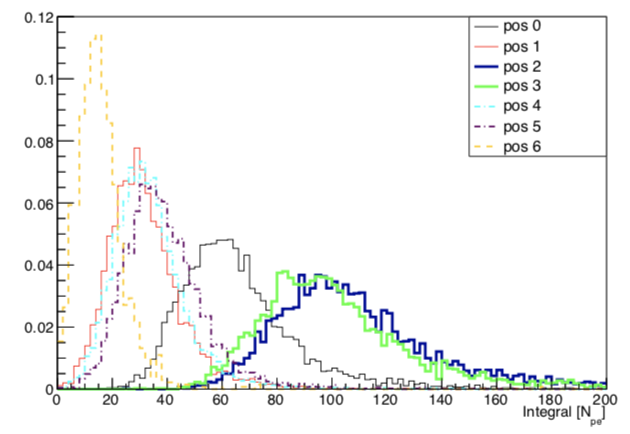
\includegraphics[width=0.45\columnwidth]{figs/DecaySpectrometer/SBT.png}
\caption{Left: prototype of a WOM MODULE, tested at the T2 H2 CERN-SPS area.
  Right: Number of photoelectrons detected by the WOM module for muons at different beam positions.}
\label{fig:SBT}
\end{figure}
%
Each cell of the LS-SBT is readout by two wavelength-shifting optical modules (WOM) detecting the scintillation light emitted in the range between 340 nm and 400 nm and transporting the light to a ring of 24 SiPMs of 3 x 3 mm$^2$ area directly coupled to the WOM tube. There are O(2000) WOMs for the whole LS-SBT. Test beam measurements in 2017 using a cell with a volume of 50 x 50 x 30 cm$^2$ (and 1.5 g/l PPO) show that a detection efficiency for muons of at least 99.6\% is achieved, if one WOM (equipped with a lightguide and viewed by an array of eight 6 x 6 mm$^2$ SiPMs, as shown in Figure\ref{fig:SBT}, left) is required to detect at least five photoelectrons. The average number of photoelectrons detected by this WOM depends on the position of the particle traversing the LS cell and was measured to be at least 30 (see Figure\ref{fig:SBT}, right). The measurements also demonstrate that a time resolution of 1 ns is achieved when two WOMs with a threshold of two photoelectrons are required.
Since the WOM-based LS-SBT principle has been demonstrated to work with good performance, the option with large-area PMTs is currently not further pursued. 

Several improvements (like increasing the PPO concentration and the direct coupling of the SiPMs to the WOM tube without using a lightguide) to increase the detected light yield and hence the efficiency have been identified, which can also improve the time resolution due to the higher photoelectron statistics. The new design will be tested in a testbeam measurement in October 2018 using a larger cell size of 120 x 80 x 30 cm$^3$. These testbeam measurements will also test a small-scale version of the LS filling system and first versions of the two readout-electronics options. Moreover, first studies will be performed whether individual SiPM readout provides any information on the original direction of the primary scintillation photon hitting the WOM tube.

While the basic components of the LS mixture have been identified (solvent LAB, fluor PPO), the exact composition still has to be optimized to the dimensions of the SBT cells. This concerns the concentration of PPO and a possible addition of paraffin oil to increase transparency vs. scintillation light yield. Reflective coating covering the inner walls of the cells have to be selected based on material compatibility and spectral reflectivity. Moreover, we will test vitamin C as an additive to improve the chemical durability of the LS towards accidental exposure to atmospheric oxygen. Finally, the use of green-sensitive SiPMs would allow to use a green dye in the WOM coatings and in turn to add a further wavelength shifter (bisMSB) to the scintillator, improving transparency and thus light response homogeneity. 

In FairSHiP, the cell geometry is implemented and the LS-SBT detector response provides the energy deposit from charged particles inside each individual cell. In the data analysis, a minimum amount of energy deposition (typically 45 MeV, which is slightly below the energy deposition of a MIP traversing a LS cell perpendicular to the vacuum vessel wall) is required to consider a LS cell as fired. Timing information taking into account testbeam results have not been yet implemented in the LS-SBT response.

The information of the LS-SBT has been used in background suppression studies of DIS events in the decay-vessel walls induced by either neutrinos or muons, assuming that the detection probability inside a LS cell of charged particles depositing at least 45 MeV is 99.9\%. The testbeam measurement results are already very close to this value. (In future studies, the energy threshold in the individual cells will be lowered, e.g. to 10 MeV, and instead it will be required that the sum of energy depositions in adjacent LS cells is above a certain threshold of O(45 MeV), since the energy deposition of one particle in the SBT is not necessarily contained in one SBT cell.)

\noindent {\bf ST}\\
\noindent
The purpose of the SHiP Spectrometer Tracker\footnote{%
   The SST was called Hidden Sector spectrometer in the Tecnhical Proposal.
   }
(SST) 
is to reconstruct with high efficiency the tracks
of charged particles from the decay of hidden particles, while rejecting background events.
Additionally, the SST must provide an accurate determination of the track
momentum and of the flight direction within the fiducial decay volume.
The precision of the extrapolated position of the tracks must be well matched with the
segmentation of the timing detectors (see section~\ref{sec:timing_detectors}) such that
the high accuracy of the associated track time can be used to remove combinatorial background.
The invariant mass, the vertex quality, the timing, the matching to background taggers
and the pointing to the production target are crucial tools for rejecting background. 
% from spurious $V^0$ meson decays, neutrino interactions or from random combinations.

The spectrometer consists of a large aperture dipole magnet  
%(discussed in Section~\ref{sec:spectrometermagnet})
and two tracking telescopes on each side of the magnet, 
%A layout with four tracking stations symmetrically arranged around the dipole magnet,
%as depicted in Figure~\ref{fig:spectrometer-layout},  is taken as a baseline.
%The size and layout of the tracker stations is connected to the size of the magnet.
%A dipole spectrometer magnet with a horizontal gap of 5~m, a height of 10~m
%and a length of 5~m provides good acceptance coverage and is considered
%feasible at a reasonable cost. % (see section \ref{sec:spectrometermagnet}).
%The $B$ field is about 0.14~T at its maximum and about 0.08~T at the location of the
%closest tracker stations, just outside the magnet.
%On the longitudinal axis the field integral between the second and third station
%is approximately 0.65~Tm.
each composed of two tracking stations. 
The four stations are identical with a nominal acceptance of 5~m in X and 10~m in Y
and based on ultra-thin straw drift tubes oriented horizontally.
Each station contains four views, in a Y-U-V-Y arrangement, where U and V are stereo views
with straws rotated by a small angle $\pm\theta_{\rm stereo}$ around the Z axis with respect to
the Y-measuring straws.
The straw veto station at the beginning of the hidden sector decay volume was removed
after demonstrating that no loss in performance of background rejection could be obtained by using 
other detector information, see section~\ref{sec:background_studies}.

The main change since the TP is the increase of the straw diameter $D$ from 10~mm to 20~mm.
This change is motivated by the refined background rate simulations (see section \ref{sec:background_rates}) 
which confirm that for $D=20~$mm the rate per straw remains modest ({\color{red}XXX~kHz TO BE CHECKED} 
in the hottest straw).
Tools for producing 20~mm straws were developed and several prototype straws,
using as before a $36~\mu$m thick PET film coated with 50~nm Cu and 20~nm Au,
were produced with no new difficulty encountered compared to fabrication of 
the original 10~mm straws. 
Several straws of 20~mm diameter and 5~m length were fabricated.
The rupture overpressure was measured on ten samples of 50~cm length and,
as shown in Fig.~\ref{fig:rupture_pressure_straws_D20mm}, was found to be around 4.4~bar, 
as expected.
% TEMUR: confirm overpressure! 
This is considered a sufficient margin for operating the straws at a pressure of about 1~bar in vacuum.
The torsion of 5~m long straws, cemented on one side and pressurized to 1~bar overpressure,
was measured and a rotation of 38 degrees was found at the free end.
A torque of about $0.076~{\rm N\,m}$  was needed to cancel the rotation.
A 2~m long $D=20~$mm straw was fabricated  and its performance as a MIP detector
was characterized in a testbeam run in the SPS north area 
as a function of wire offset at nominal conditions ($\sim 1.05$~bar pressure, 
70\% Ar / 30\% CO$_2$).
First results indicate that a straw hit resolution of $120~\mu$m is achievable with high 
hit efficiency and over most of the straw diameter, independently of the wire offset,
as visible in figure~\ref{Fig:straw_resolution_TB2017}.
The drift time spectra for different wire offsets were analyzed and methods are being investigated
to extract the local wire offset from the distinctive features of the spectra.
Alignment studies for the full detector, using MC simulation, are being started, which should allow
us to define the geometrical constraints for the mechanical engineering design.

\begin{figure}[htb]
\begin{center}
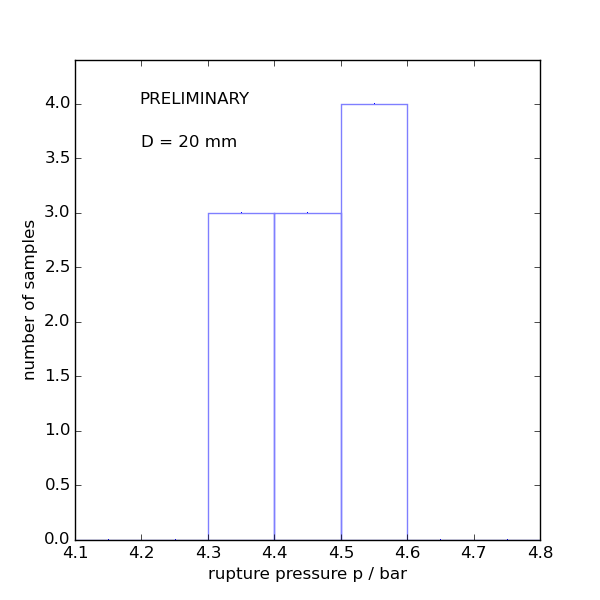
\includegraphics[width=0.5\textwidth]{figs/DecaySpectrometer/rupture_pressure_straws_D20mm.png}
\caption{Rupture overpressure for straw samples with diameter $D=20~$mm.}
\label{fig:rupture_pressure_straws_D20mm}
\end{center}
\end{figure}

\begin{figure}[htb]
\begin{center}
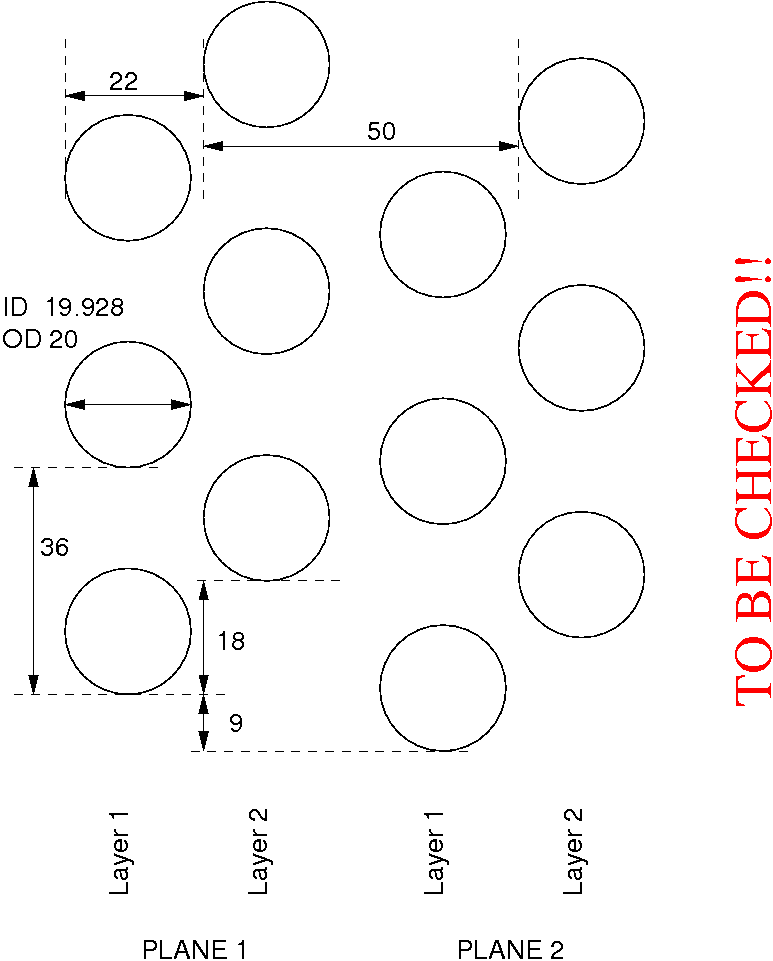
\includegraphics[width=0.5\textwidth]{figs/DecaySpectrometer/straw-layout-SHiP.png}
\caption{New SST straw layout for straw diameter $D=20~$mm as used in FairShip.}
\label{Fig:straw-layout-SHiP}
\end{center}
\end{figure}

\begin{figure}[htb]
\begin{center}
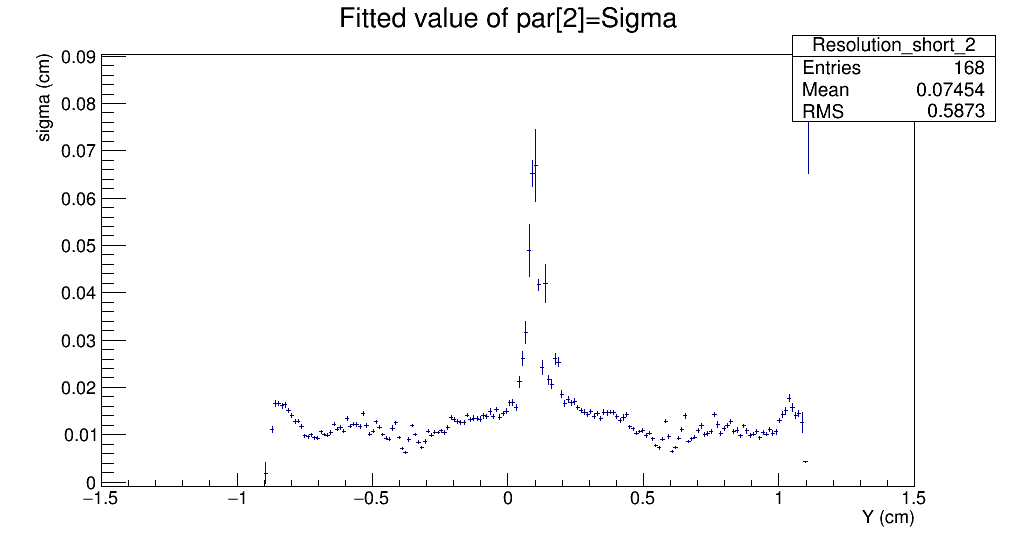
\includegraphics[width=0.45\textwidth]{figs/DecaySpectrometer/sigmaS_328.png} % - the smallest offset 0.02 mm
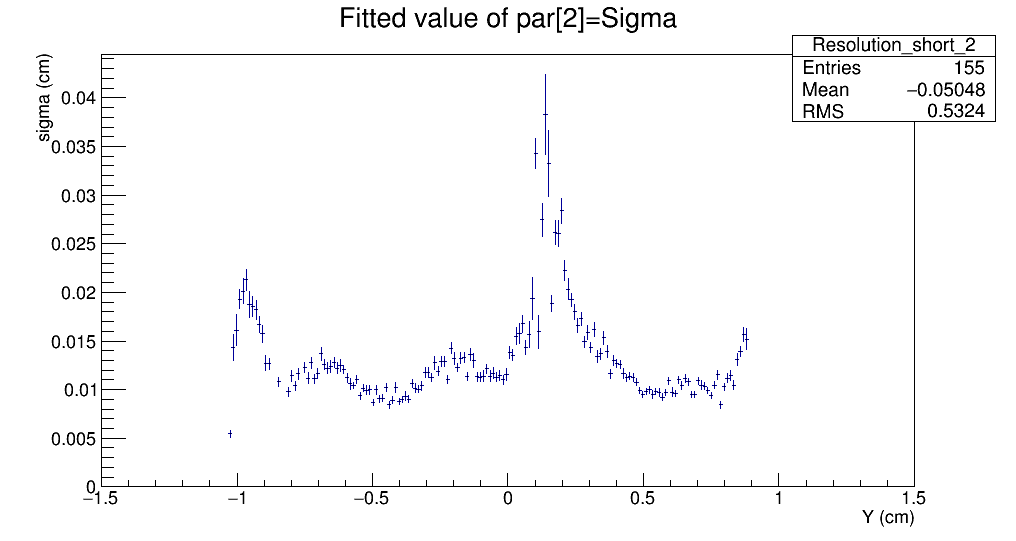
\includegraphics[width=0.45\textwidth]{figs/DecaySpectrometer/sigmaS_163.png} % - the largest offset 1.97 mm
\caption{{\color{red} PRELIMINARY}. Hit resolution across the straw diameter for $D=20$~mm. 
Left: no wire offset. right: wire offset of $\sim 2~$mm.}
\label{Fig:straw_resolution_TB2017}
\end{center}
\end{figure}

Several changes of the SST in FairShip were made and studies are under way.
The straw layout was updated to take into account the larger straw diameter (20~mm), 
see figure~\ref{Fig:straw-layout-SHiP}.
As shown in  section ~\ref{sec:performance}),  the performance of the SST is not degraded 
in comparison to the TP.
Dummy mechanical frames (stainless steel) were added around the straw views, to provide a more realistic
material environment, and it was checked that background rates remain acceptable. 
A new field map, extracted from an FEA calculation, was implemented in the MC simulation, 
including the return field in the yoke. The return field has an effect on the rates
in the last two stations, though these remain acceptable.
An optimization of the station geometry and, in particular, of the stereo angle is ongoing.

The engineering challenges associated with the mechanical properties of strongly tensioned 
long straws and tungsten wires were considered \cite{PietNotes}.
Elongation and relaxation effects, which if neglected would result in excessive
and evolving sagging of the straws, must be taken into account {\sl ab inito} in the design.
Several schemes are being studied, one including a long-stroke constant-force spring,
capable of maintaining the wire under the desired tension while
accomodating a straw elongation of several centimeters, 
and another one utilizing a straw suspension mechanism based on carbon fibres.
A radically different method, developed for the COSY-TOF detector and the PANDA straw  tube 
tracker \cite{PANDA_TDR}, is now also being explored. In this technique, ultrathin straws are held 
together by sparse glue dots in a close-packing configuration and ``inflated'' to 1~bar overpressure.
A self-supporting, rigid an straight straw tube module
can be obtained without externally tensioning the straws and without straw suspension mechanism.

A preliminary conceptual design of the vacuum enclosure is being worked out
which foresees a vacuum chamber with rectangular cross section, longitudinally extending 
over the whole spectrometer length and provided with four rectangular openings on the top side.
These openings are used to lower the tracker station frames, fully equiped, into the vacuum volume.
In this concept, the vacuum enclosure is decoupled from the mechanical structures
for the detector. 
Front-end electronics are located inside the vacuum and require active cooling.

PietNotes:\\
- ``Elastic stability and HEP detectors: a primer'', P. Wertelaers, EP-Tech-Note-2018-005.\\
- ``Anode wire in cylindrical cathode tube : destabilizing electrostatic force'', P. Wertelaers, EP-Tech-Note-2018-003.\\
- ``Pipe regarded as bending beam : destabilizing transverse effect of internal pressure'', P. Wertelaers, EP-Tech-Note-2018-002. 

PANDA:\\
- ``Technical Design Report for the PANDA (AntiProton Annihilations at Darmstadt) Straw Tube Tracker''
   W. Erni et al., Eur. Phys. J. A (2013) 49: 25, DOI 10.1140/epja/i2013-13025-8.\\



Additional pictures:


\begin{figure}[htb]
\begin{center}
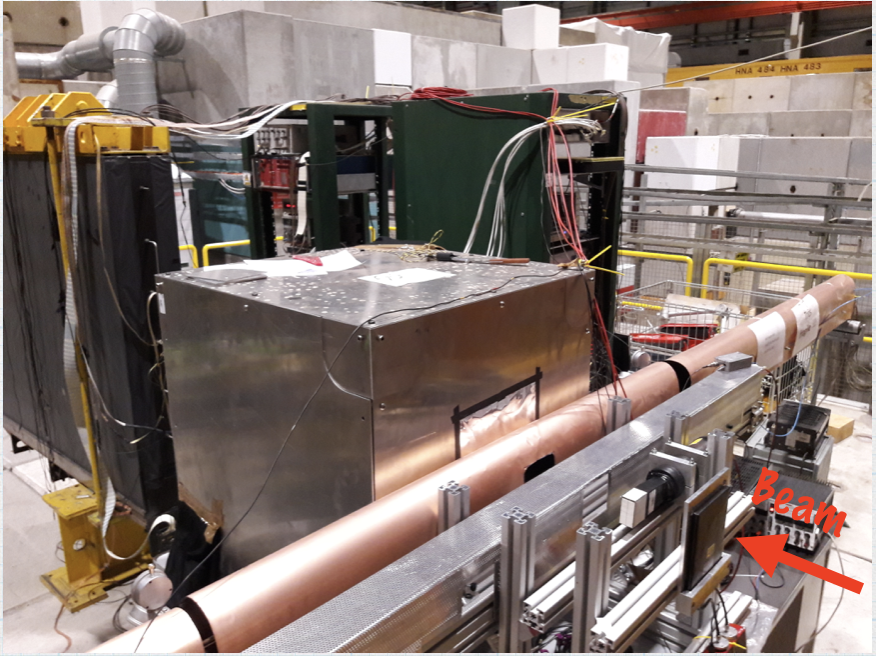
\includegraphics[width=0.45\textwidth]{figs/DecaySpectrometer/SST_TB_setup_2017.png}
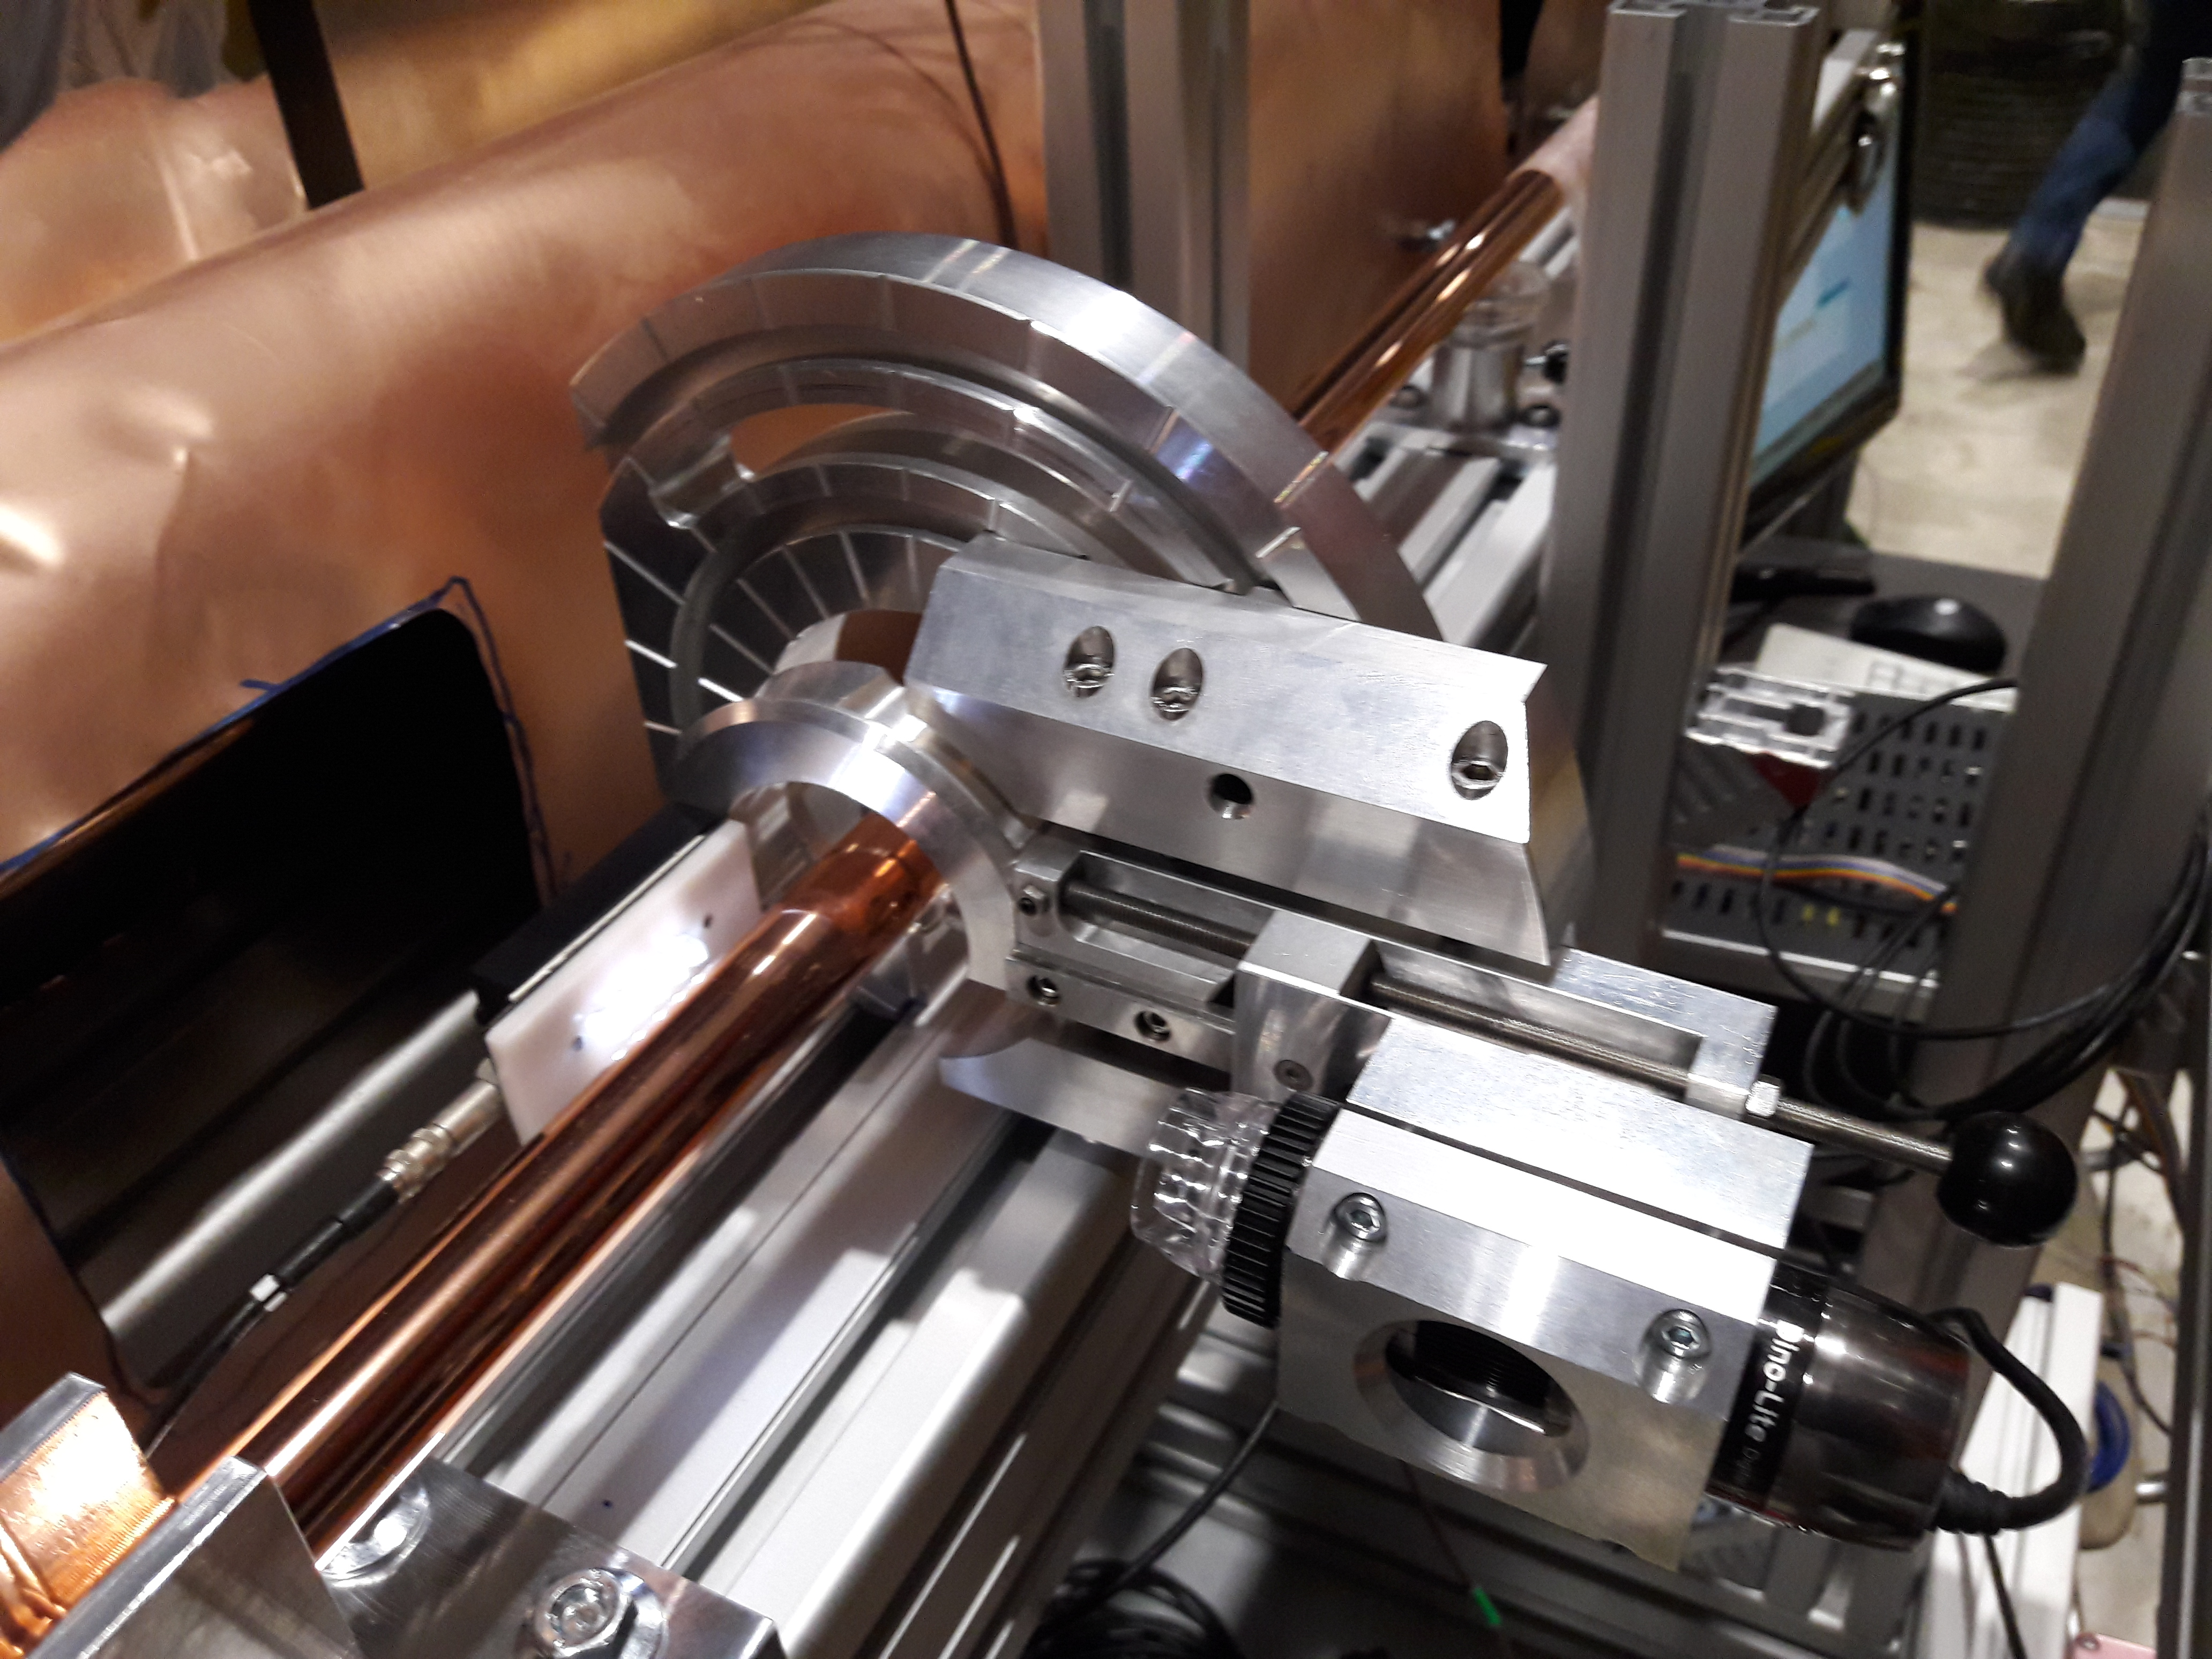
\includegraphics[width=0.45\textwidth]{figs/DecaySpectrometer/20170918_152403.jpg}
\caption{Left: picture of test beam setup. Labels could be added. 
         Right: zoom on straw while wire offset is measured with digital camera.}
\label{Fig:pictures_TB2017}
\end{center}
\end{figure}


\noindent {\bf Timing detector}\\
\noindent
The TP baseline configuration for the plastic scintillator-based option for the SHiP timing detector (TD) consisted of two columns of 305~cm long bars instrumented with PMTs. Although the viability of using large-area SiPMs for the light readout was not known at the time, this scheme was discussed as an attractive one which needed R\&D. It is now demonstrated that the large-area SiPM scheme is not only viable, but actually offers a better performance at a lower cost. A three-column setup of bars read out by arrays of large-area SiPMs is now chosen as the baseline option. 
%
\begin{figure}[h]
\centering
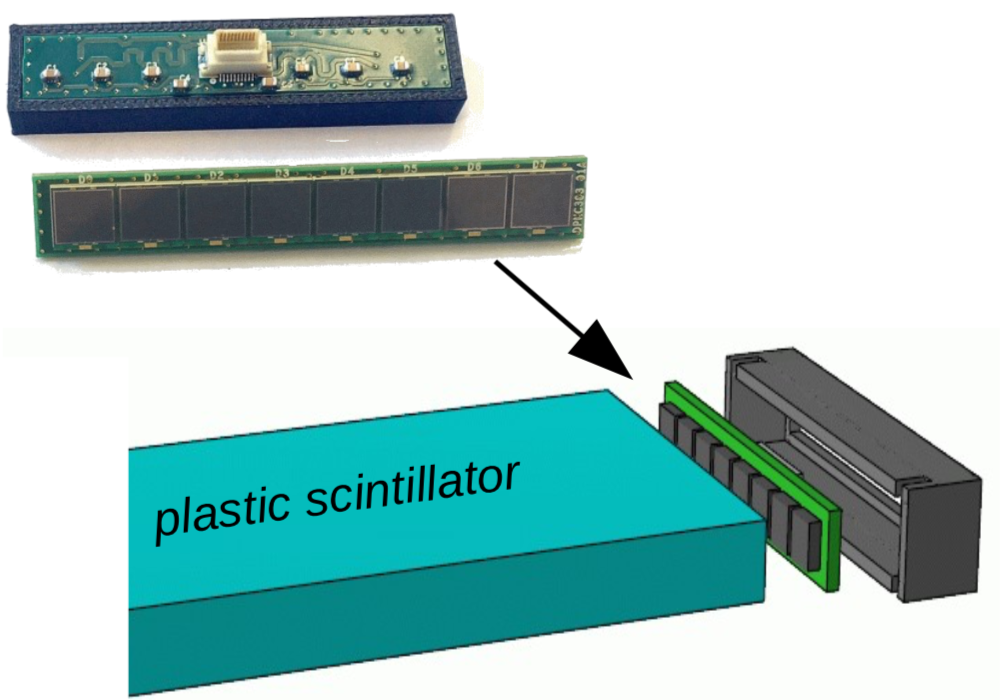
\includegraphics[width=0.35\columnwidth]{figs/DecaySpectrometer/TD_SiPM.png}
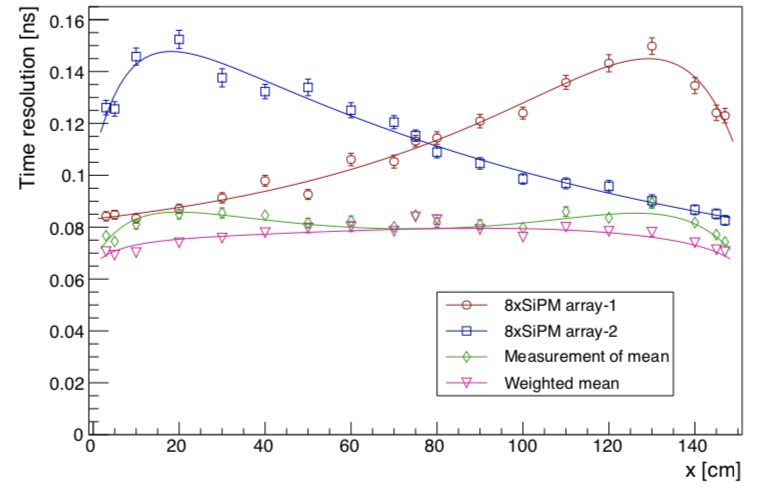
\includegraphics[width=0.55\columnwidth]{figs/DecaySpectrometer/TD_dt.png}
\caption{Left: picture of an array of eight 6~mm$\times$6~mm SiPMs integrated into a PCB with a parallel connection and applied directly to the bar surface. Right: time resolution as measured by the
SiPM arrays at both ends of a 1.5~m bar measured as a function of the beam impact position along the bar~\cite{Betancourt:2017sex}.}
\label{fig:TD}
\end{figure}
%
The current SHiP TD design features bars made of EJ-200 plastic scintillator with dimensions 168~cm$\times$6~cm$\times$1~cm, arranged in three columns and 182 rows with 0.5~cm overlap between bars, for a total area of 5~m$\times$10~m. Each bar is read out on both sides by an array of eight 6~mm$\times$6~mm SiPMs; the signals from the eight SiPMs are summed by an ASIC to form a single channel. Thus there are a total of 564 bars and 1128 channels.  

Figure\ref{fig:TD} presents the results obtained with a 1.5~m long bar read out by two arrays of 8 SiPMs attached to both ends of the bar, as detailed in Ref.~\cite{Betancourt:2017sex}. The resolution of the mean time is demonstrated to be $\sim$80~ps along the whole length of the bar. In Summer 2018, a 22-bar (44 channels) prototype array with 1.68~m long bars (same dimensions as those of the current SHiP TD design) was successfully operated at CERN PS test beams, providing time-of-flight information to a high-pressure TPC prototype. It showed similar timing performance as the single bar over its 2.1~m$ ^2$ active area.

A slightly more modest resolution of $\sim$100 ps has been obtained at the cosmic test of the MRPC prototype representing an alternative option for the TD. 

\noindent {\bf Calorimeter system}\\
\noindent

\noindent {\bf Muon system}\\
\noindent
The muon system has to identify muons with high efficiency ($> 95\%$) and reduce the hadron contamination to less than ${\bf xx} \%$
in a momentum range between $\sim 5-100 $ GeV/c. Moreover it will help the timing detector in rejecting
the combinatorial muon background pairs from the muon halo by requiring a tight ($<$ 1 ns) time coincidence of the two muon tracks:
in fact halo muons are expected to be spread along the whole spill length (1 sec) while muons coming from the same mother particle
are coincident in time.

The muon detector is placed downstream of the calorimeter systems and comprises four stations of active layers
interleaved by three muon filters.
The four stations are 6~m wide, 12~m high  and are placed downstream the calorimeter system.
The amount of material of the calorimeter system corresponds to { 6.7~$\lambda_I$ }. 
The muon filters are iron walls 60~cm thick corresponding to { 3.4~$\lambda_I$ each}.
A muon with normal incidence must have an energy at least of 2.6~GeV/c to reach the first muon station 
and at least 5.3~GeV/c to reach the last muon station.
The multiple scattering of  muons in the material of the calorimeter system and the muon filters drives the 
granularity of the system. Simulation studies show that a readout granularity of $\sim$10 cm in the transverse directions
is adequate for the interesting momentum range.

The active detectors of the muon system will cover a surface of $\sim 288 $ m$^2$ divided in four stations.
The baseline technology chosen for the active layers for the Technical proposal~\cite{Anelli:2015pba}
was extruded plastic scintillator bars with wavelength-shifter (WLS) fibres 
and silicon photo-multipliers (SIPMs) readout. A thoughrough R\&D has been carried out on this technology and the results
have been summarized in Ref.~\cite{Montanari:2016rmo}: a time resolution of $\sim$800 ps has been measured on bars 3 m long
fully dominated by the jitter of the fiber scintillation time.
The highly non uniform and relatively large hit rate, and the request of achieving
a sub-ns time resolution for reducing the combinatorial background led us to consider a different technology
for the muon system: scintillating tiles with direct SIPMs readout.
% - reasons for this choice:
This option has several advantages:
\begin{itemize}
\item[-] it provides an intrinsic better time resolution due to the absence of the jitter due to the fiber scintillation time;
\item[-] it is much robust with respect to hit rate variations;
\item[-] it provides $x,y$ coordinates without complicated crossings/corrections;
\item[-] it is of much easier mechanical construction (no grooves, no glue, no fine matching fiber-SIPM);
\item[-] it allows for a one-to-one correspondence physical-electronic channel, in the assumption of having one
  FEE channel per tile.
\end{itemize}

An excellent time resolution of $\sim 340$ ps has been measured on
small tiles prototypes, as shown in Figure~\ref{fig:tile}, right. As a consequence,
a muon system made of four stations equipped with scintillating tiles can in principle reach $\sim 200$ ps time resolution,
if the results obtained on small prototypes can be extrapolated to a large scale detector.
A new test beam campaign planned in October 2018 will allow us to further progress on this R\&D.
%
\begin{figure}[htb]
\centering
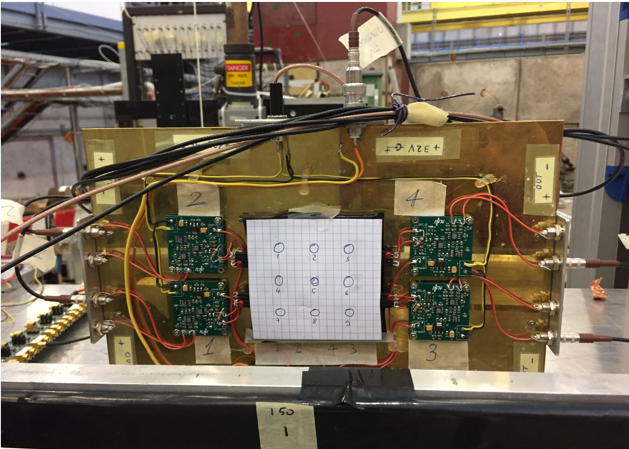
\includegraphics[width=0.45\columnwidth]{figs/DecaySpectrometer/tile_on_TB.png}
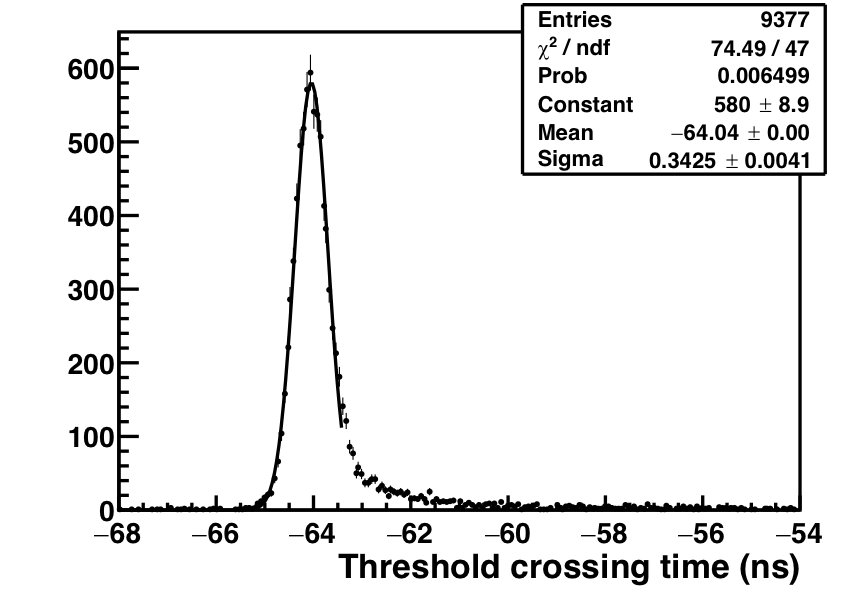
\includegraphics[width=0.45\columnwidth]{figs/DecaySpectrometer/time_reso.png}
\caption{Left: prototype of a tile for the muon system, tested at the T10 area, CERN-PS.
  Right: time resolution.}
\label{fig:tile}
\end{figure}
%
Scintillating tiles with direct SIPM readout is now the baseline solution for the SHiP Muon system.
The basic parameters of the system are summarized in Table~\ref{tab:muon_layout} assuming a preliminary tile dimension
of $10\times20\times1$ cm$^3$. The tiles geometry has been implemented in the SHiP Monte Carlo
at the digitization level, where the tiles are simulated side by side without dead spaces (see Figure~\ref{fig:muon_system}, right).
The choice of having the tiles at the digitization level and not hard-coded in the GEANT geometry
is driven by the request of having a geometry very flexible to be able to follow the upcoming test beam
results and the  evolution of the mechanical drawings of the system without rerun the (computationally heavy) GEANT simulation.
Given the excellent time resolution, the possibility of building the muon system with only three stations instead of four
is currently being considered and a final decision will be taken for the TDR.
% - table with main parameters:
\begin{table}[htbp]
\caption{Muon System layout as implemented in FairSHiP.}
\label{tab:muon_layout}
\vspace{.1cm}
\begin{center}
\begin{small}
\begin{tabular}{lr}
\hline
number of active stations  & 4 \\
active stations dimensions  & ($600 \times 1200 \times 1$) cm$^3$ \\
tile dimensions   & ($10 \times 20 \times 1$) cm$^3$ \\
number of tiles   &  3 600 $\times$ 4 = 14,400\\
weight of the scintillator & 11.52 t \\
FEE channels      &  14, 400 \\ \hline
number of passive iron filters   & 3 \\
filters dimensions  & $ (600 \times 1200 \times 60) $ cm$^3$ \\
iron weight   & $\sim$1000 t \\
\hline
\end{tabular}
\end{small}
\end{center}
\end{table}


\subsection{Detector performance}
\label{DSperformance}


%\begin{figure}[htb]
%\centering
%\includegraphics[width=0.9\linewidth]{figs/XXXXX.pdf}
%\caption{}
%\label{fig:XXXXX}
%\end{figure}

%\section{Physics Performance}
\label{sec{physicsperformance}}

\subsection{Sensitivity to hidden sector particles}

\subsection{Sensitivity to LDM}
\begin{itemize}
    \item Simulation of LDM production and interaction: MadDump and FairShip (Figure \ref{fig:ldm_prod})
    
    \begin{figure}[htbp]
    \centering  
    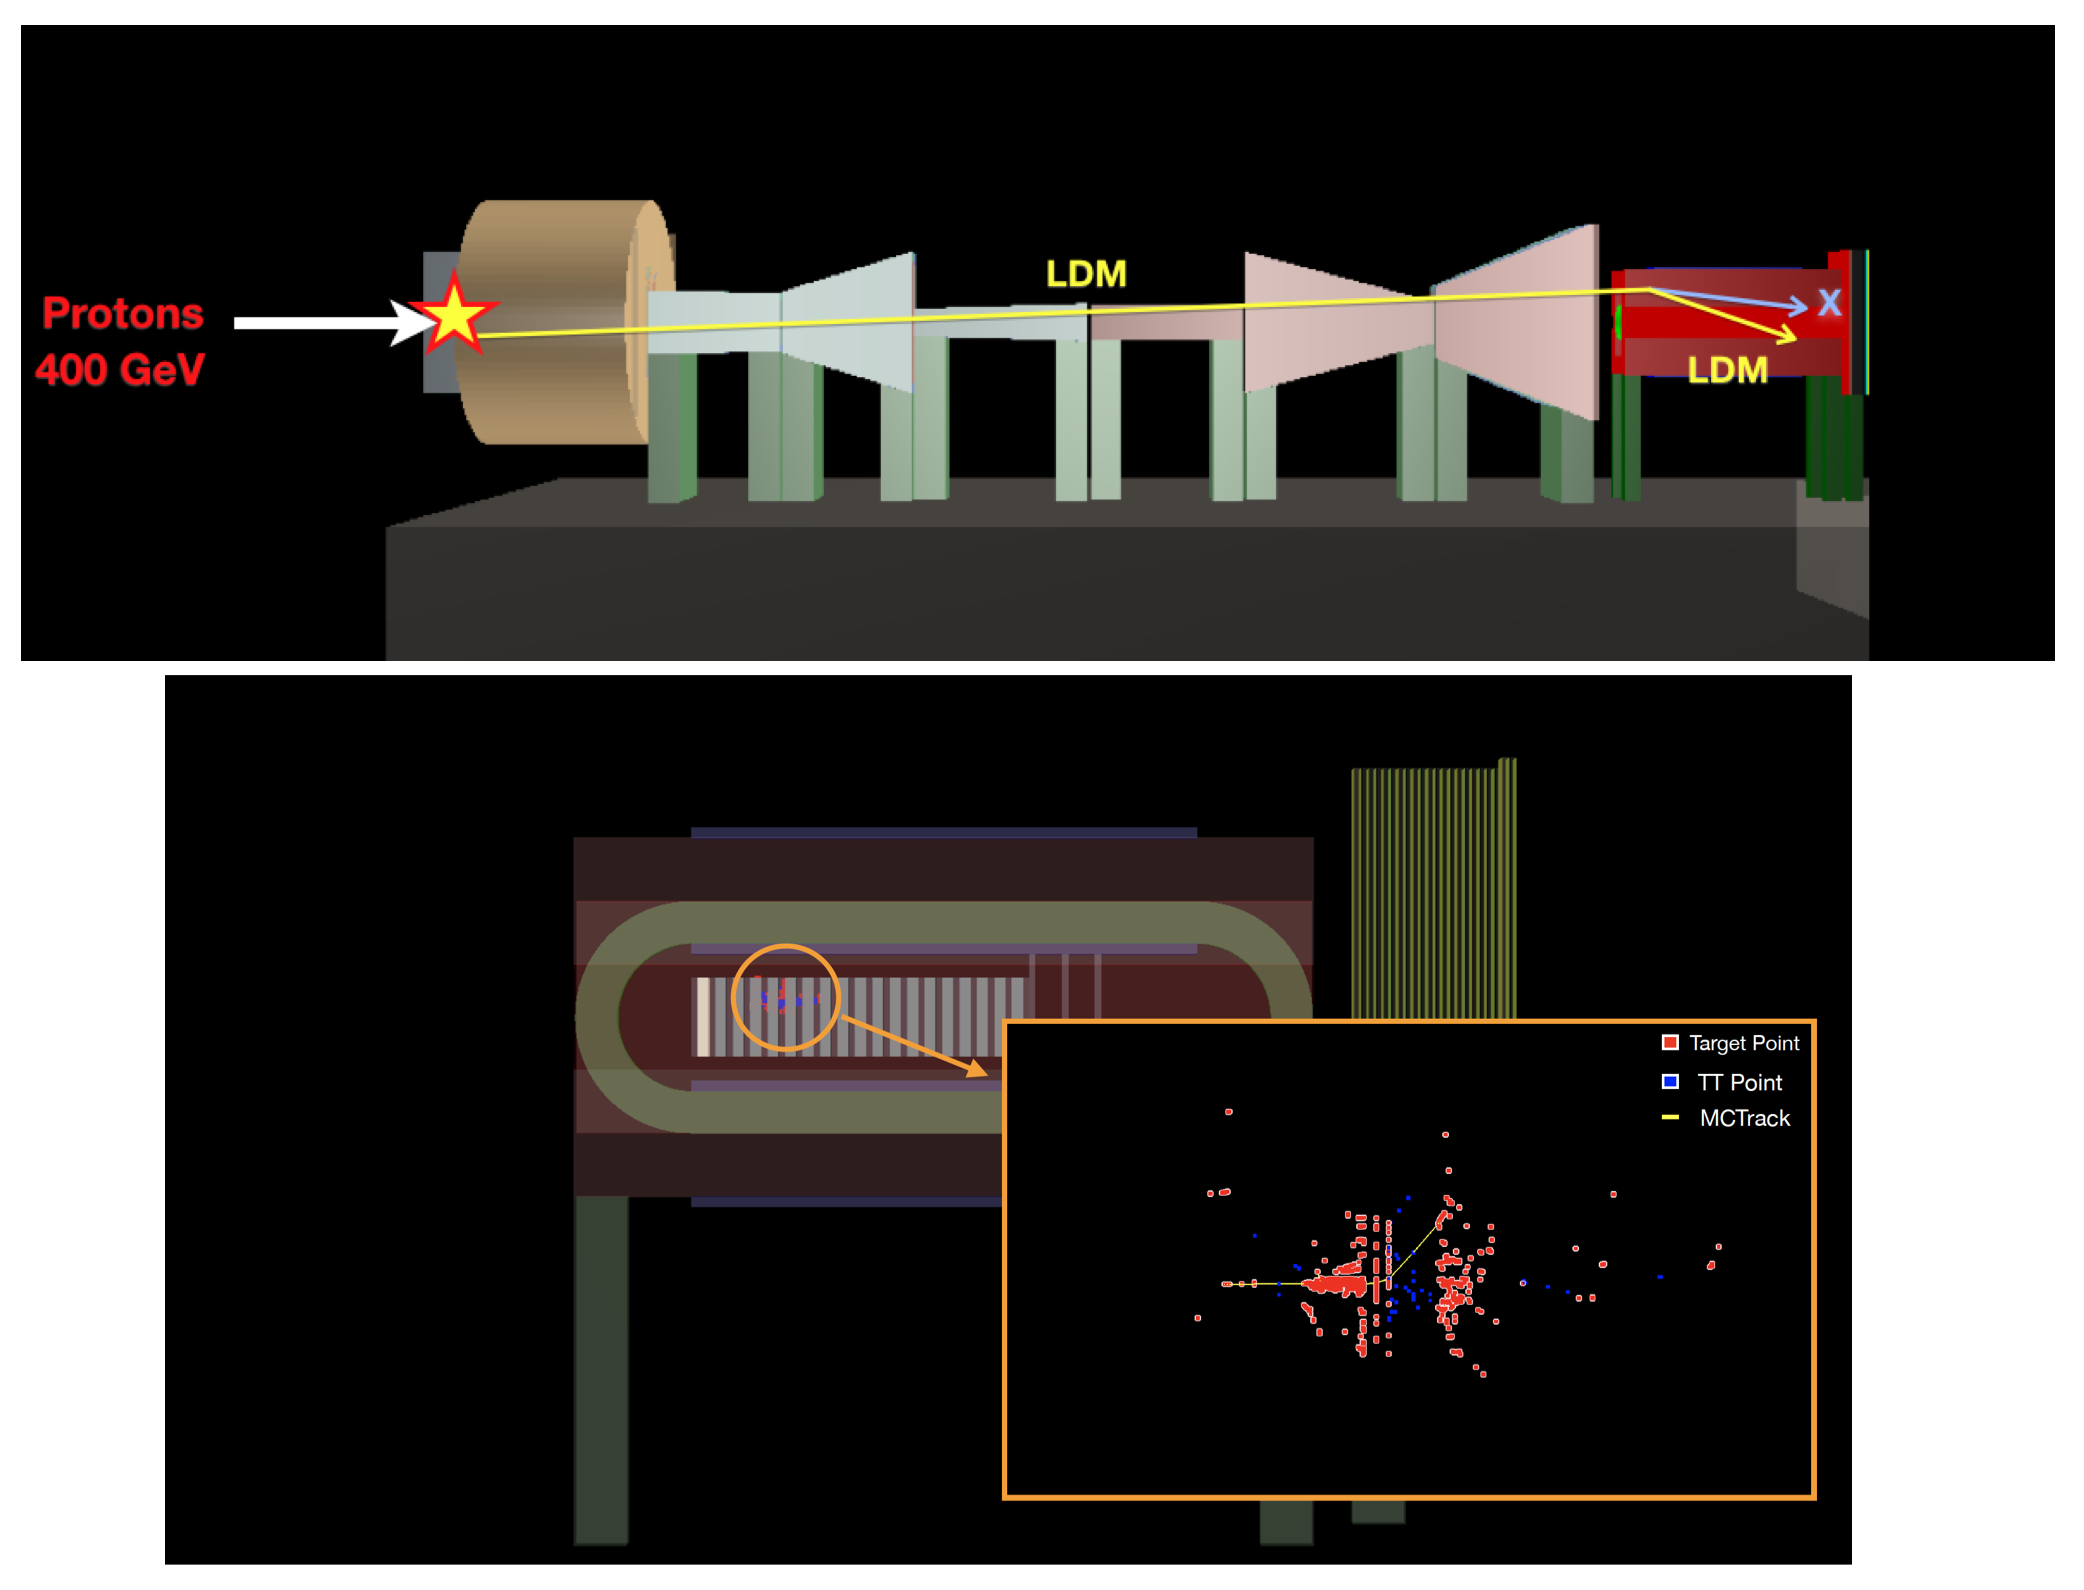
\includegraphics[scale=0.3]{figs/PhysicsPerformance/LDM_Prod.png}
    \caption{Light Dark Matter simulation process design in two steps. The first one is handled by MadDump and concerns the BSM particle production and consequent decay/interaction inside the detector; the second stage consists in the particles propagation inside the SHiP detector and is owned by FairShip.}
    \label{fig:ldm_prod}
    \end{figure}

    \item Neutrino background yield estimation
    \begin{itemize}
        \item[$\circ$] Kinematic distribution for neutrino background (Figure \ref{fig:ldm_back})
         \item[$\circ$] Selection criteria: 1 GeV $< E_e <$ 20 GeV, 10 mrad $<\theta_e<$ 20 rad
   \item[$\circ$] Neutrino background yield (Table \ref{tab:ldm_back})
    
      \begin{figure}[htbp]
    \centering  
    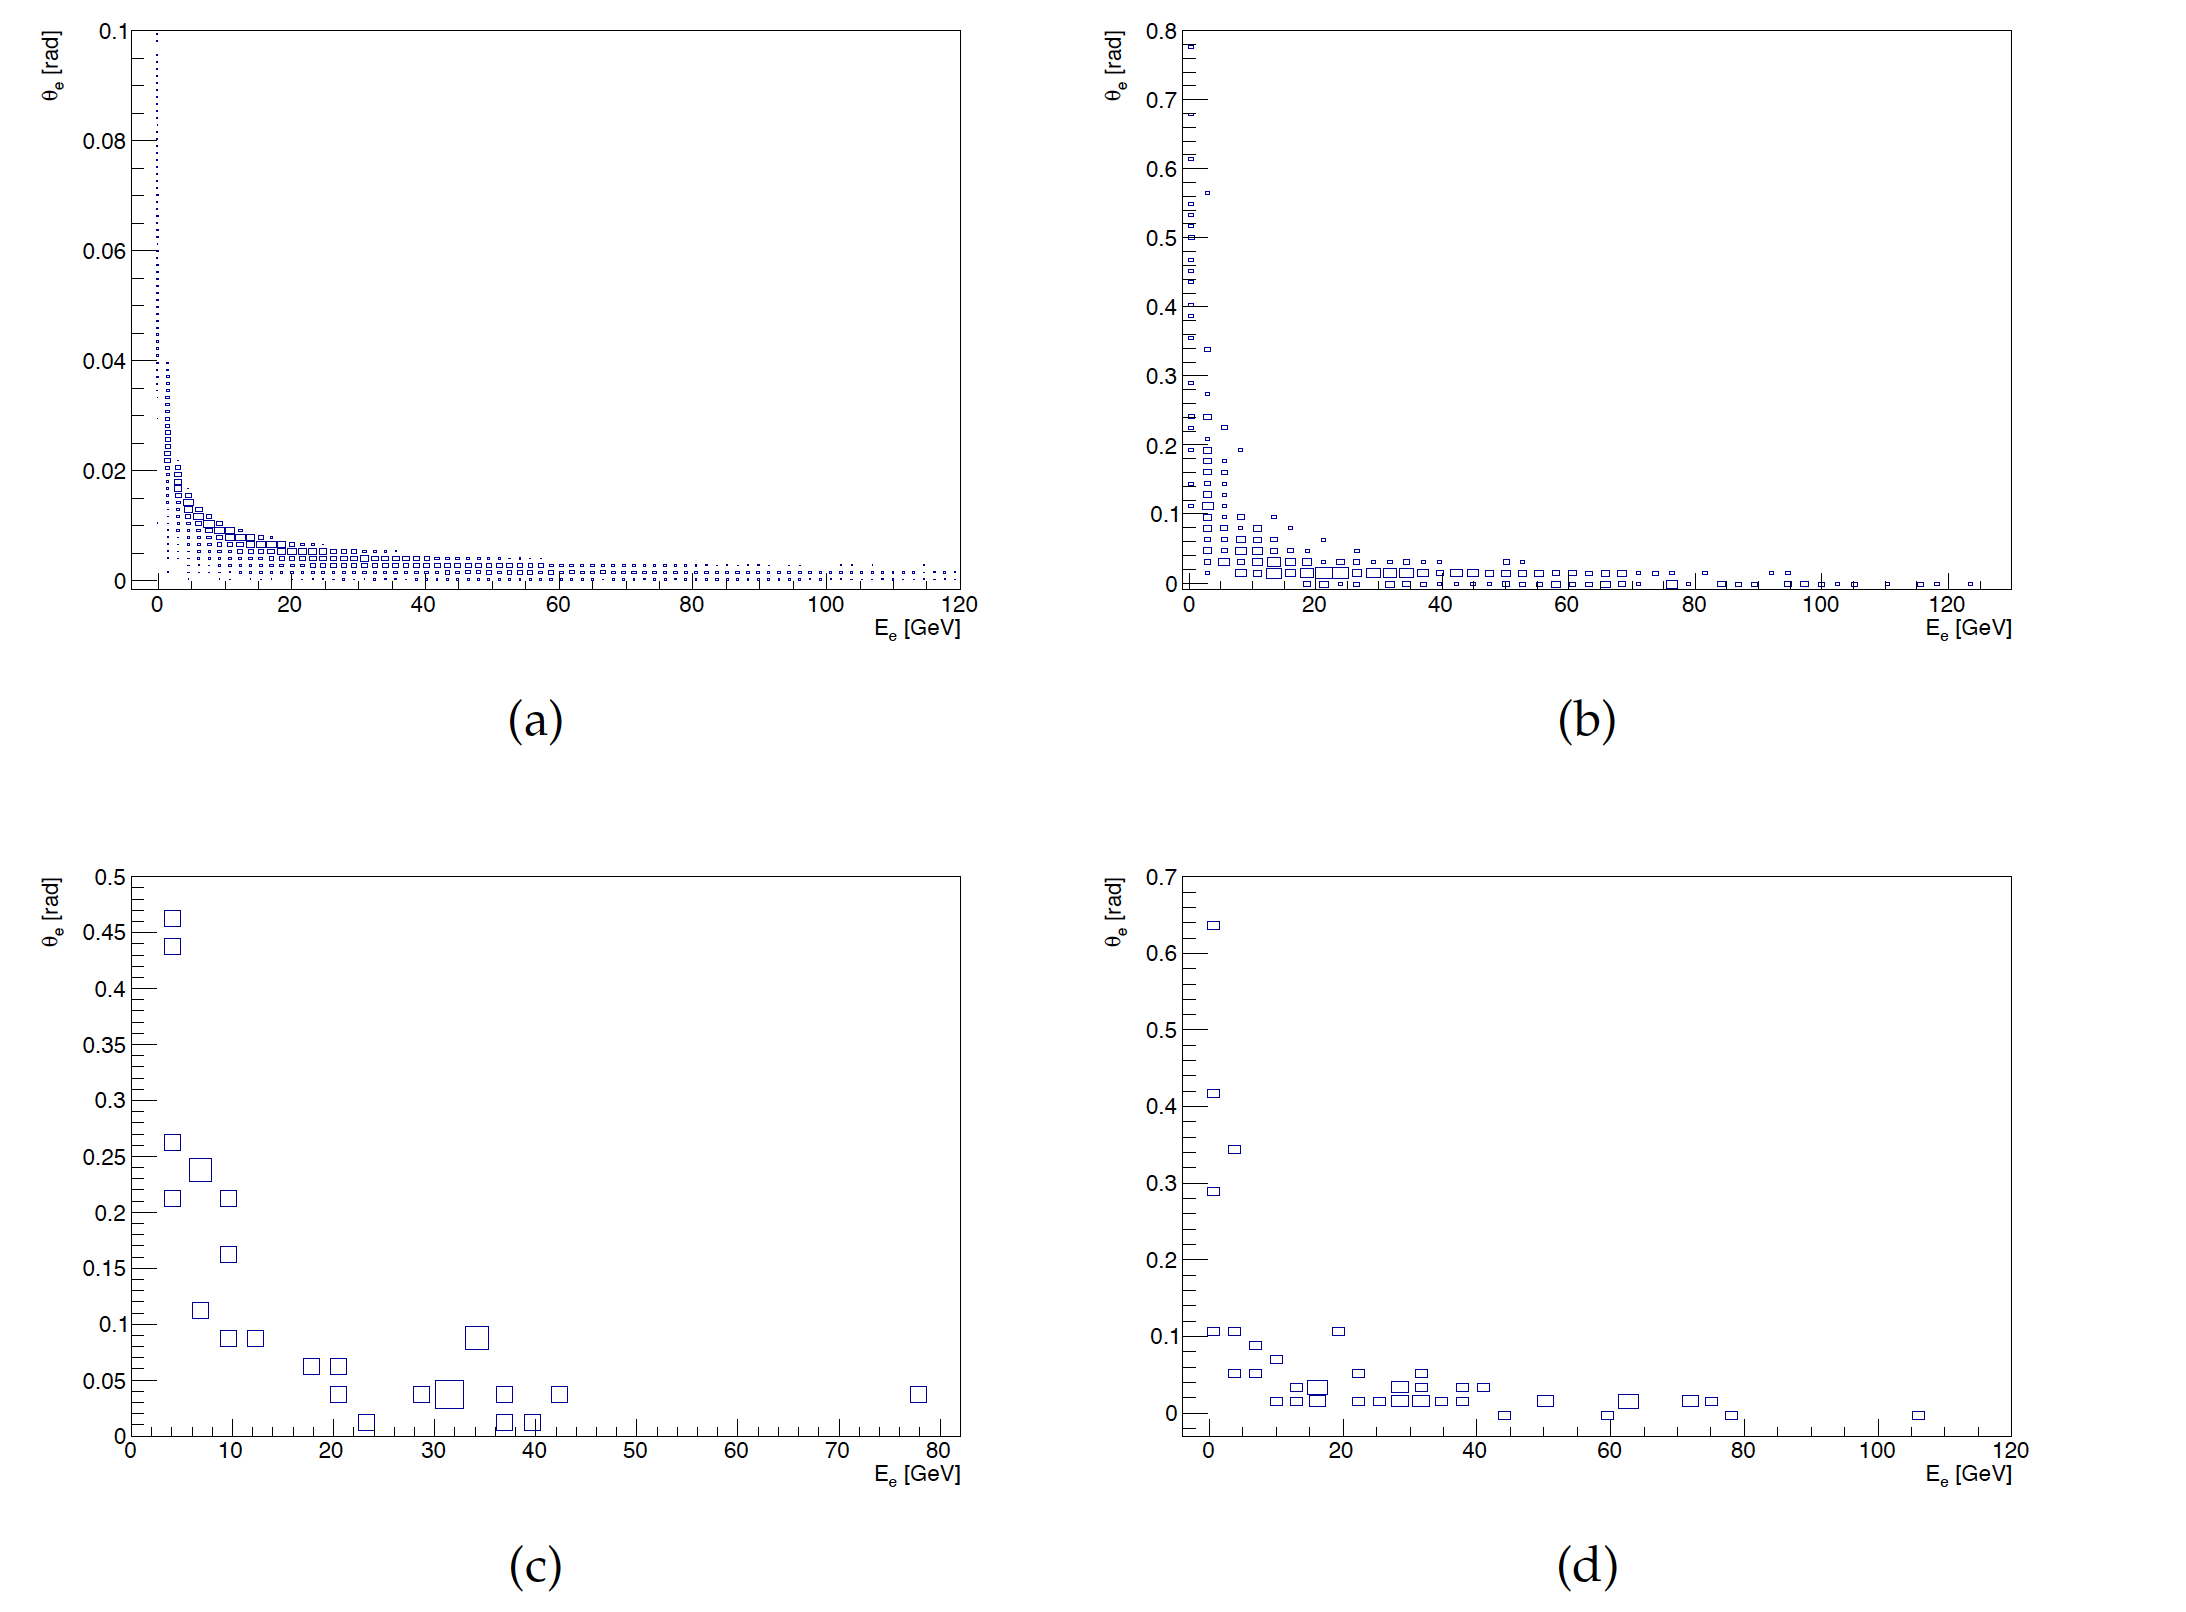
\includegraphics[scale=0.3]{figs/PhysicsPerformance/LDM_back.png}
    \caption{Electron scattering angle w.r.t. the incoming neutrino direction versus the electron energy in case of: (a) elastic, (b) quasi-elastic, (c) deep inelastic and (d) resonant scattering.}
    \label{fig:ldm_back}
    \end{figure}
    
    \begin{table}[htbp]
    \begin{center}
    \begin{tabular}{llllll}
    \hline
    & $\nu_e$ & $\bar{\nu_e}$ & $\nu_\mu$ & $\bar{\nu_\mu}$   & all  \\
    \hline
    Elastic Scattering on $e^-$   & 81  & 45  & 56 & 35 & 217\\
    Quasi-elastic Scattering      & 245 & 236 & -  & -  & 481 \\
    Resonant Scattering           & 16  & 162 & -  & -  & 178\\
    Deep Inelastic Scattering     &  -  & 14  & -  & -  & 14\\
    \hline
    total                         & 342 & 457 & 56  & 35& 890\\
 
    \end{tabular}
    \label{tab:ldm_back}
    \caption{Number of  background events for LDM search after cuts with 2$\times 10^{20}$ p.o.t.}  
    \end{center}
    \end{table}

    
     \end{itemize}
     
    \item Sensitivity to LDM
    \begin{itemize}
        \item[$\circ$] Model used for the simulation
        \item[$\circ$] Exclusion plot (Figure \ref{fig:ldm_sensitivity})
   \end{itemize}
    
     \begin{figure}[htbp]
    \centering  
    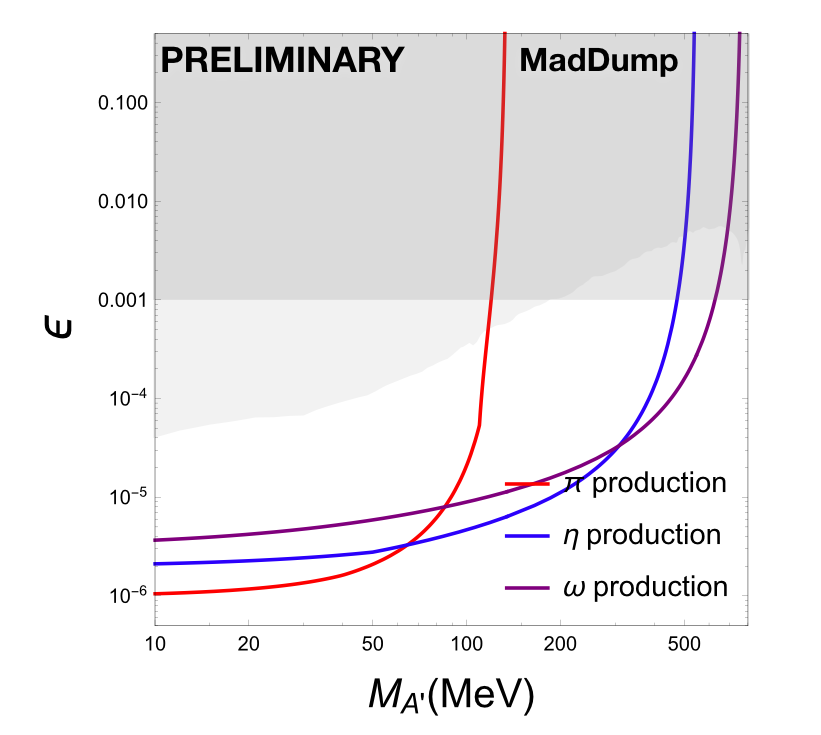
\includegraphics[scale=0.3]{figs/PhysicsPerformance/newsens.png}
    \caption{SHiP estimated sensitivity to Light Dark Matter from Dark Photon $A'$ decays in the plane ($\epsilon$, $M_{A'}$ ), in case the latter is produced in the decay of mesons. The grey shaded regions determine the parameter space which has been already ruled out by BaBar and MiniBooNE searches.}
    \label{fig:ldm_sensitivity}
    \end{figure}
    
    
\end{itemize}




\subsection{Physics with neutrinos}

\begin{itemize}
    \item Neutrino yield estimation
        \begin{itemize}
        \item[$\circ$] Energy spectra for different neutrino flavors  (Figure \ref{fig:neu_spectra})
        \item[$\circ$] Neutrino yield for different neutrino flavors  (Table \ref{tab:neu_yield})
        \item[$\circ$] Expected $\nu_\tau$ and $\overline{\nu}_\tau$ yield in different decay channels
         (Table \ref{tab:tau_yield})
        \end{itemize}

 \begin{figure}[htbp]
    \centering  
    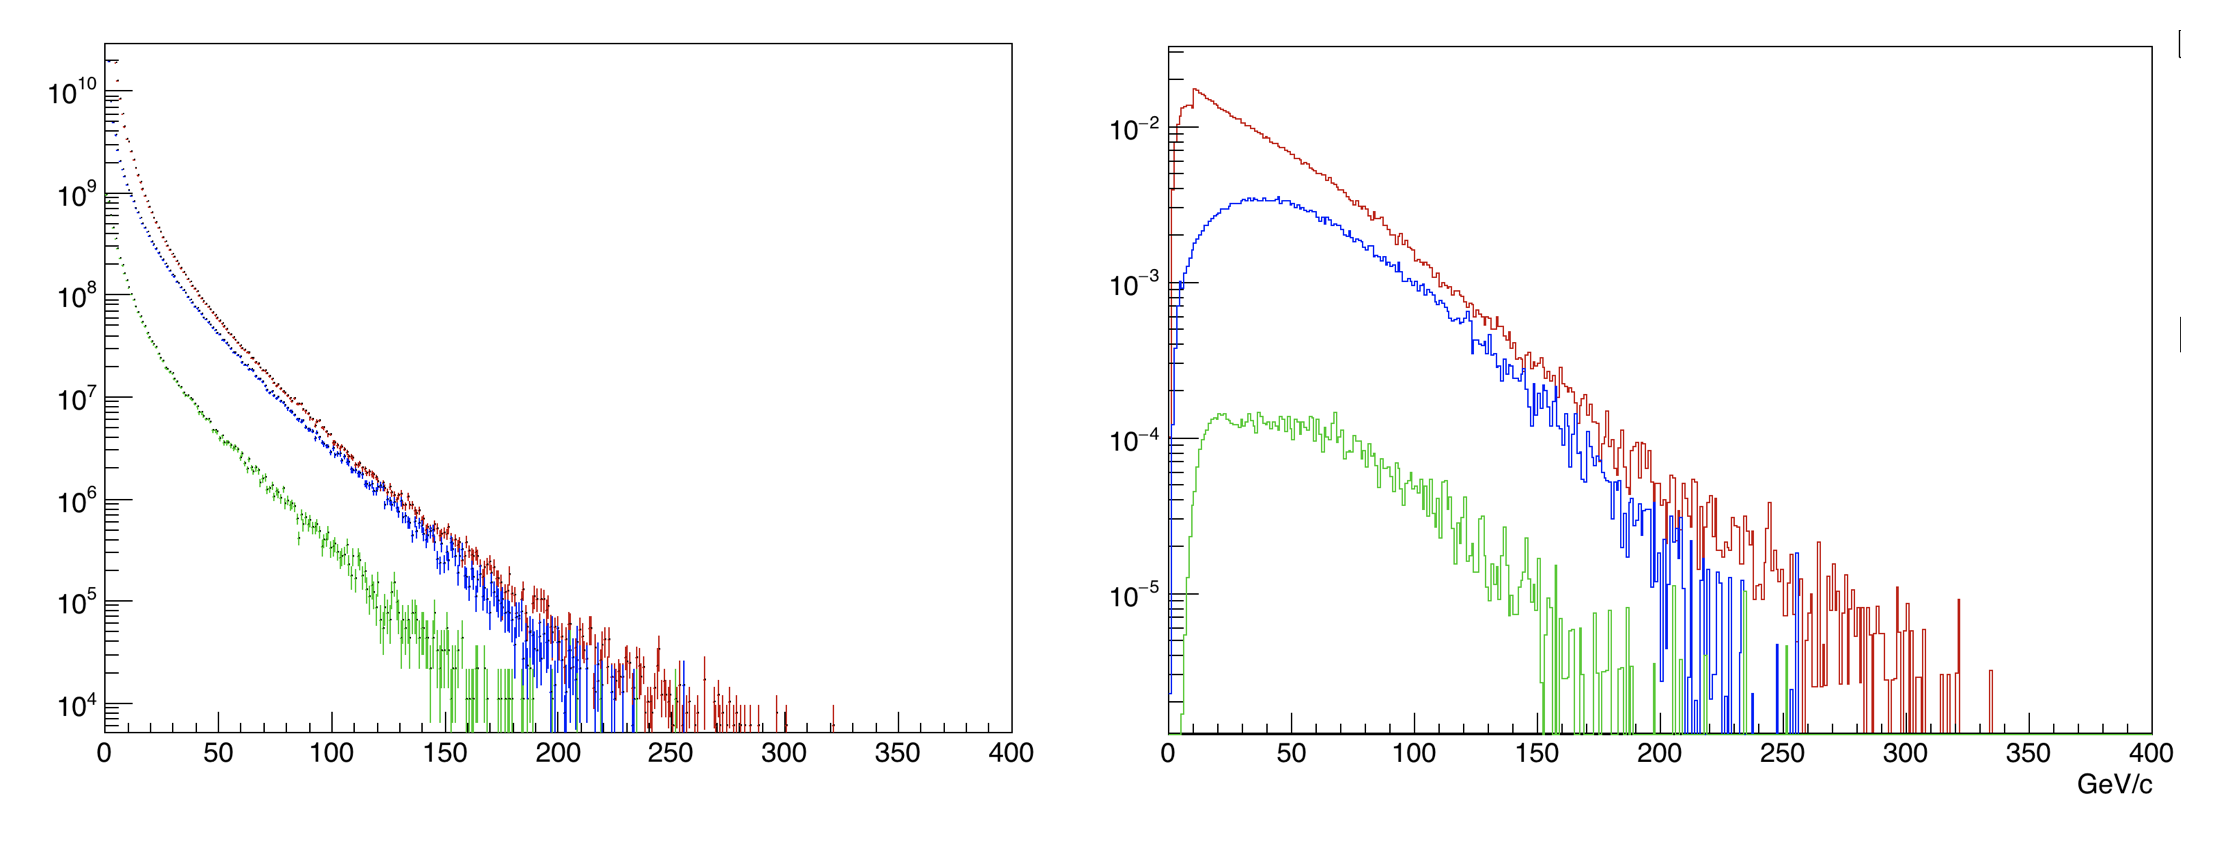
\includegraphics[scale=0.4]{figs/PhysicsPerformance/neu_spectra.png}
    \caption{Energy spectra of the different neutrino flavors  at the beam dump (left) and charged-current deep-inelastic interactions (right).}
    \label{fig:neu_spectra}
    \end{figure}
    
\begin{table}[htp]
\begin{center}
\begin{tabular}{c | c c  | c c  }
\hline
& $<$E$>$  & Beam  & $<$E$>$ &  CC DIS\\
&       (GeV) & dump  & (GeV) & interactions \\
 \hline
 $N_{\nu_e}$                 & 4.1 & $2.8 \times 10^{17}$    & 59 & $1.1 \times 10^{6}$ \\
 $N_{\nu_\mu}$               & 1.5 & $4.2 \times 10^{18}$    & 42 & $2.7 \times 10^{6}$ \\
 $N_{\nu_\tau}$              & 7.4 & $1.4 \times 10^{16}$    & 52 & $3.2 \times 10^{4}$ \\
 $N_{\overline{\nu}_e}$      & 4.7 & $2.3 \times 10^{17}$    & 46 & $2.6 \times 10^{5}$ \\
 $N_{\overline{\nu}_\mu}$    & 1.6 & $2.7 \times 10^{18}$    & 36 & $6.0 \times 10^{5}$ \\
 $N_{\overline{\nu}_\tau}$   & 8.1 & $1.4 \times 10^{16}$    & 70 & $2.1 \times 10^{4}$ \\
 \hline
\end{tabular}
\end{center}
\caption{Integrated neutrino yield for $2\times10^{20}$ p.o.t. for the  different neutrino flavors at the beam dump (left) and charged-current deep-inelastic interactions (right).}
\label{tab:neu_yield}
\end{table}

\begin{table}[htp]
\begin{center}
\begin{tabular}{c | c| c }
\hline
  decay channel &  $\nu_\tau$  & $\overline{\nu}_\tau$  \\
                    
 \hline
 $\tau \to \mu$  & 1200 & 1000 \\
 $\tau \to h$      & 4000  & 3000 \\
 $\tau \to 3h$    & 1000  & 700 \\

 \hline
 total & 6200 & 4700  \\
 \hline
 \end{tabular}
 \end{center}
 \caption{Expected number of $\nu_\tau$ and $\overline{\nu}_\tau$ signal events observed in the different $\tau$ decay channels, except the $\tau \to e$, where the lepton number cannot be determined.}
 \label{tab:tau_yield}
 \end{table}
 
\end{itemize}




%\section{Project plan}
\label{sec:projectplan}

\begin{itemize}
    \item Project plan in synch with BDF plan
    \item Extra year of stop of SPS (last year of LS3)
    \item commission of facility and experiment after LS3
    \item prototyping plan (reference to document - update?)
    \item COSTING detector, rough statements about impact of changes and expectation for total cost, no detailed breakdown if any at all
    \item safety file and planning
\end{itemize}

The detector R&D schedule, TDR, PRR, production.

The schedule is elaborated in more detail in the BDF Yellow Book~\cite{ref:bdf_yellowbook}

The schedule for the SHiP experiment and the experimental facility is largely driven by the CERN long-term accelerator schedule. Accordingly, the schedule aims at profiting as much as possible from data taking during Run 4 (currently 
2027--2029). 

Most of the experimental facility can be constructed in parallel to operating the North Area beam facilities. The connection to the SPS has been linked to Long Shutdown 3 (i.e. for LHC 2024--2026) but requires that the stop of the North Area is extended by one year (2025--2026). The schedule requires preparation of final prototypes and the TDRs for both the detector and the facility by beginning 2022, and construction and installation between 2023 and beginning 2027.  

% The second half of the dedicated transfer line, the target area and the experimental area can be 
% constructed in parallel to operating the current North Area beam facilities. In order to minimize the
% impact on the North Area, the connection to the SPS requiring the construction of a junction cavern 
% and the installation of the new splitter and beam line, has been linked to Long Shutdown 3. Since the 
% time required for this work is estimated to 2 years, the stop of the North Area must be extended by 
% one year (2025–2026).




%\section{Status of the SHiP Collaboration}
\label{sec:collaboration}

The SHiP Expression of Interest was submitted to SPSC in October 2013. This was followed by the Technical Proposal submitted to the SPSC in April 2015. The SHiP Technical Proposal was successfully reviewed by the SPSC and the CERN RB up to March 2016, with a recommendation to prepare a Comprehensive Design Study report by 2019.

SHiP is currently a collaboration of 53 institutes and 4 associated institutes, in  total representing 18 countries, CERN and JINR. The formal organisation of SHiP consists of a Country Representative Board (CRB), Interim spokesperson, Technical Coordinator and Physics Coordinator, and the group of project conveners as elected and ratified by the CRB. The organisation has been adopted for the Comprehensive Design Study phase.  


\bibliographystyle{JHEP} %
\bibliography{thesis} %
\bibliography{SimulationBiblio} %

% \begin{thebibliography}{99}
% \end{thebibliography}

\end{document}
